% 2020 May 18 - THE MARTIAN ATMOSPHERIC BOUNDARY LAYER - https://agupubs.onlinelibrary.wiley.com/doi/10.1029/2010RG000351

% 2020 Oct 8 - ICC FOV = 120 deg, alpha = 10 * 0.82 mrad/px = 8.2 mrad = 0.14 deg
% https://mars.nasa.gov/insight/spacecraft/about-the-lander/#cameras
% https://www.nature.com/articles/s41467-020-14679-1
%
% D^{50%}_{\rm act} = 35 m

% Asurvey ~ (120 deg)(35 m)^2/(2*(0.14 deg)^2) = 3.8 km^2
% Seeing no dust devils means the areal density < 1/3.8 km^2 ~ 

% From Golombek+ (2020 - https://www.nature.com/articles/s41467-020-14679-1):
% A slope to the north limits the horizon to about 50 m away (Supplementary Fig. 5); it is topped by three rocks (The Pinnacles), and eolian bedforms (Dusty ridge) near the southwest rim of a ~100 m diameter degraded impact crater (Figs. 3–5). To the east-southeast (Fig. 4), the horizon extends about 400 m to the rim of a relatively fresh, ~100 m diameter impact crater (Sunrise) with large eolian bedforms on its rim (The Wave). The rim of a larger (460 m diameter), relatively fresh crater can be seen on the east-southeast horizon ~2.4 km away (Distant Crater in Fig. 6b).

%% Beginning of file 'sample63.tex'
%%
%% Modified 2019 June
%%
%% This is a sample manuscript marked up using the
%% AASTeX v6.3 LaTeX 2e macros.
%%
%% AASTeX is now based on Alexey Vikhlinin's emulateapj.cls 
%% (Copyright 2000-2015).  See the classfile for details.

%% AASTeX requires revtex4-1.cls (http://publish.aps.org/revtex4/) and
%% other external packages (latexsym, graphicx, amssymb, longtable, and epsf).
%% All of these external packages should already be present in the modern TeX 
%% distributions.  If not they can also be obtained at www.ctan.org.

%% The first piece of markup in an AASTeX v6.x document is the \documentclass
%% command. LaTeX will ignore any data that comes before this command. The 
%% documentclass can take an optional argument to modify the output style.
%% The command below calls the preprint style which will produce a tightly 
%% typeset, one-column, single-spaced document.  It is the default and thus
%% does not need to be explicitly stated.
%%
%%
%% using aastex version 6.3
\usepackage{amsmath}
\usepackage{wrapfig}
\documentclass{aastex63}

%% The default is a single spaced, 10 point font, single spaced article.
%% There are 5 other style options available via an optional argument. They
%% can be invoked like this:
%%
%% \documentclass[arguments]{aastex63}
%% 
%% where the layout options are:
%%
%%  twocolumn   : two text columns, 10 point font, single spaced article.
%%                This is the most compact and represent the final published
%%                derived PDF copy of the accepted manuscript from the publisher
%%  manuscript  : one text column, 12 point font, double spaced article.
%%  preprint    : one text column, 12 point font, single spaced article.  
%%  preprint2   : two text columns, 12 point font, single spaced article.
%%  modern      : a stylish, single text column, 12 point font, article with
%% 		  wider left and right margins. This uses the Daniel
%% 		  Foreman-Mackey and David Hogg design.
%%  RNAAS       : Preferred style for Research Notes which are by design 
%%                lacking an abstract and brief. DO NOT use \begin{abstract}
%%                and \end{abstract} with this style.
%%
%% Note that you can submit to the AAS Journals in any of these 6 styles.
%%
%% There are other optional arguments one can invoke to allow other stylistic
%% actions. The available options are:
%%
%%   astrosymb    : Loads Astrosymb font and define \astrocommands. 
%%   tighten      : Makes baselineskip slightly smaller, only works with 
%%                  the twocolumn substyle.
%%   times        : uses times font instead of the default
%%   linenumbers  : turn on lineno package.
%%   trackchanges : required to see the revision mark up and print its output
%%   longauthor   : Do not use the more compressed footnote style (default) for 
%%                  the author/collaboration/affiliations. Instead print all
%%                  affiliation information after each name. Creates a much 
%%                  longer author list but may be desirable for short 
%%                  author papers.
%% twocolappendix : make 2 column appendix.
%%   anonymous    : Do not show the authors, affiliations and acknowledgments 
%%                  for dual anonymous review.
%%
%% these can be used in any combination, e.g.
%%
%% \documentclass[twocolumn,linenumbers,trackchanges]{aastex63}
%%
%% AASTeX v6.* now includes \hyperref support. While we have built in specific
%% defaults into the classfile you can manually override them with the
%% \hypersetup command. For example,
%%
%% \hypersetup{linkcolor=red,citecolor=green,filecolor=cyan,urlcolor=magenta}
%%
%% will change the color of the internal links to red, the links to the
%% bibliography to green, the file links to cyan, and the external links to
%% magenta. Additional information on \hyperref options can be found here:
%% https://www.tug.org/applications/hyperref/manual.html#x1-40003
%%
%% Note that in v6.3 "bookmarks" has been changed to "true" in hyperref
%% to improve the accessibility of the compiled pdf file.
%%
%% If you want to create your own macros, you can do so
%% using \newcommand. Your macros should appear before
%% the \begin{document} command.
%%
\newcommand{\vdag}{(v)^\dagger}
\newcommand\aastex{AAS\TeX}
\newcommand\latex{La\TeX}
\newcommand{\totalvortices}{990}
\newcommand{\maskedvortices}{44}
\newcommand{\largestDeltaPobs}{$\left( 8.9 \pm 0.2 \right)\,{\rm Pa}$}
\newcommand{\largestDeltaPobssol}{65}
\newcommand{\largestGammaobssol}{20}
\newcommand{\largestGammaobs}{$\left( 99 \pm 3 \right)\,{\rm s}$}
\newcommand{\boverDactltone}{88}
\newcommand{\vorticeswithnowinds}{56}
\newcommand{\numICCimages}{1527}

%% Reintroduced the \received and \accepted commands from AASTeX v5.2
\received{June 1, 2019}
\revised{January 10, 2019}
\accepted{\today}
%% Command to document which AAS Journal the manuscript was submitted to.
%% Adds "Submitted to " the argument.
\submitjournal{PSJ}

%% For manuscript that include authors in collaborations, AASTeX v6.3
%% builds on the \collaboration command to allow greater freedom to 
%% keep the traditional author+affiliation information but only show
%% subsets. The \collaboration command now must appear AFTER the group
%% of authors in the collaboration and it takes TWO arguments. The last
%% is still the collaboration identifier. The text given in this
%% argument is what will be shown in the manuscript. The first argument
%% is the number of author above the \collaboration command to show with
%% the collaboration text. If there are authors that are not part of any
%% collaboration the \nocollaboration command is used. This command takes
%% one argument which is also the number of authors above to show. A
%% dashed line is shown to indicate no collaboration. This example manuscript
%% shows how these commands work to display specific set of authors 
%% on the front page.
%%
%% For manuscript without any need to use \collaboration the 
%% \AuthorCollaborationLimit command from v6.2 can still be used to 
%% show a subset of authors.
%
%\AuthorCollaborationLimit=2
%
%% will only show Schwarz & Muench on the front page of the manuscript
%% (assuming the \collaboration and \nocollaboration commands are
%% commented out).
%%
%% Note that all of the author will be shown in the published article.
%% This feature is meant to be used prior to acceptance to make the
%% front end of a long author article more manageable. Please do not use
%% this functionality for manuscripts with less than 20 authors. Conversely,
%% please do use this when the number of authors exceeds 40.
%%
%% Use \allauthors at the manuscript end to show the full author list.
%% This command should only be used with \AuthorCollaborationLimit is used.

%% The following command can be used to set the latex table counters.  It
%% is needed in this document because it uses a mix of latex tabular and
%% AASTeX deluxetables.  In general it should not be needed.
%\setcounter{table}{1}

%%%%%%%%%%%%%%%%%%%%%%%%%%%%%%%%%%%%%%%%%%%%%%%%%%%%%%%%%%%%%%%%%%%%%%%%%%%%%%%%
%%
%% The following section outlines numerous optional output that
%% can be displayed in the front matter or as running meta-data.
%%
%% If you wish, you may supply running head information, although
%% this information may be modified by the editorial offices.
\shorttitle{Vortices and Meteorology from InSight}
\shortauthors{Jackson}
%%
%% You can add a light gray and diagonal water-mark to the first page 
%% with this command:
%% \watermark{text}
%% where "text", e.g. DRAFT, is the text to appear.  If the text is 
%% long you can control the water-mark size with:
%% \setwatermarkfontsize{dimension}
%% where dimension is any recognized LaTeX dimension, e.g. pt, in, etc.
%%
%%%%%%%%%%%%%%%%%%%%%%%%%%%%%%%%%%%%%%%%%%%%%%%%%%%%%%%%%%%%%%%%%%%%%%%%%%%%%%%%
\graphicspath{{./}{figures/}}
%% This is the end of the preamble.  Indicate the beginning of the
%% manuscript itself with \begin{document}.

\begin{document}

\title{Inferring Vortex and Meteorological Statistics from InSight}

%% LaTeX will automatically break titles if they run longer than
%% one line. However, you may use \\ to force a line break if
%% you desire. In v6.3 you can include a footnote in the title.

%% A significant change from earlier AASTEX versions is in the structure for 
%% calling author and affiliations. The change was necessary to implement 
%% auto-indexing of affiliations which prior was a manual process that could 
%% easily be tedious in large author manuscripts.
%%
%% The \author command is the same as before except it now takes an optional
%% argument which is the 16 digit ORCID. The syntax is:
%% \author[xxxx-xxxx-xxxx-xxxx]{Author Name}
%%
%% This will hyperlink the author name to the author's ORCID page. Note that
%% during compilation, LaTeX will do some limited checking of the format of
%% the ID to make sure it is valid. If the "orcid-ID.png" image file is 
%% present or in the LaTeX pathway, the OrcID icon will appear next to
%% the authors name.
%%
%% Use \affiliation for affiliation information. The old \affil is now aliased
%% to \affiliation. AASTeX v6.3 will automatically index these in the header.
%% When a duplicate is found its index will be the same as its previous entry.
%%
%% Note that \altaffilmark and \altaffiltext have been removed and thus 
%% can not be used to document secondary affiliations. If they are used latex
%% will issue a specific error message and quit. Please use multiple 
%% \affiliation calls for to document more than one affiliation.
%%
%% The new \altaffiliation can be used to indicate some secondary information
%% such as fellowships. This command produces a non-numeric footnote that is
%% set away from the numeric \affiliation footnotes.  NOTE that if an
%% \altaffiliation command is used it must come BEFORE the \affiliation call,
%% right after the \author command, in order to place the footnotes in
%% the proper location.
%%
%% Use \email to set provide email addresses. Each \email will appear on its
%% own line so you can put multiple email address in one \email call. A new
%% \correspondingauthor command is available in V6.3 to identify the
%% corresponding author of the manuscript. It is the author's responsibility
%% to make sure this name is also in the author list.
%%
%% While authors can be grouped inside the same \author and \affiliation
%% commands it is better to have a single author for each. This allows for
%% one to exploit all the new benefits and should make book-keeping easier.
%%
%% If done correctly the peer review system will be able to
%% automatically put the author and affiliation information from the manuscript
%% and save the corresponding author the trouble of entering it by hand.

\correspondingauthor{Brian Jackson}
\email{bjackson@boisestate.edu}

\author[0000-0002-9495-9700]{Brian Jackson}
\author{Justin Crevier}
\author{Michelle Szurgot}
\author{Ryan Battin}
\affiliation{Department of Physics\\ 
Boise State University\\ 
1910 University Drive, Boise ID 83725-1570 USA}
\author[0000-0002-7200-5682]{Cl\'{e}ment Perrin}
\affiliation{Universit\'{e} de Paris, Institut de Physique du Globe de Paris, CNRS, Paris, France}
\author[0000-0003-1219-0641]{S\'{e}bastien Rodriguez}
\affiliation{Universit\'{e} de Paris, Institut de Physique du Globe de Paris, CNRS, Paris, France}
\affiliation{Institut Universitaire de France, Paris, France}
%% Note that the \and command from previous versions of AASTeX is now
%% depreciated in this version as it is no longer necessary. AASTeX 
%% automatically takes care of all commas and "and"s between authors names.

%% AASTeX 6.3 has the new \collaboration and \nocollaboration commands to
%% provide the collaboration status of a group of authors. These commands 
%% can be used either before or after the list of corresponding authors. The
%% argument for \collaboration is the collaboration identifier. Authors are
%% encouraged to surround collaboration identifiers with ()s. The 
%% \nocollaboration command takes no argument and exists to indicate that
%% the nearby authors are not part of surrounding collaborations.

%% Mark off the abstract in the ``abstract'' environment. 
\begin{abstract}
The InSight Mission has operated on the surface of Mars for nearly two Earth years, returning hundreds of sols worth of data, including detections of the first Marsquakes. The lander also deployed an exquisitely sensitive meteorological instrument package to assess the influence of the atmosphere on the geophysical measurements, as well as imaging cameras to monitor both instrument deployment and local surface activity. In addition to their relevance to InSight geoscience, these latter instruments have detected a variety of boundary layer phenomena, including small-scale vortices. These vortices register as short-lived ($<$ tens of seconds), negative ($<$ a few \% ambient) pressure excursions in the barometric time-series collected by InSight. These vortices closely resemble dust devils, which largely shape climate and air quality on Mars where they are widespread. Although InSight encountered more than 900 vortices and collected more than 1000 images of the martian surface, no active dust devils were imaged -- apparently, all the vortices were dustless. In spite of the lack of dust devil detections, we can leverage the vortex detections and InSight’s daily wind speed measurements to learn about the boundary layer processes that create dust devils. In this study, we will discuss our analysis of InSight’s meteorological data to assess the statistics of vortex and dust devil activity. We also able to infer the encounter distances for the vortices and, therefrom, the maximum wind speeds within the vortices. Surveying the available imagery, we place upper limits on what fraction of vortices carry dust (i.e., how many are bonafide dust devils) and estimate threshold wind speeds for dust lifting. Comparing ours results to detections of dust devil tracks seen in space-based observations of the InSight landing site, we can also infer thresholds and frequency of track formation by vortices.
\end{abstract}

%% Keywords should appear after the \end{abstract} command. 
%% See the online documentation for the full list of available subject
%% keywords and the rules for their use.
\keywords{Planetary atmospheres (1244), Mars (1007)}

%% From the front matter, we move on to the body of the paper.
%% Sections are demarcated by \section and \subsection, respectively.
%% Observe the use of the LaTeX \label
%% command after the \subsection to give a symbolic KEY to the
%% subsection for cross-referencing in a \ref command.
%% You can use LaTeX's \ref and \label commands to keep track of
%% cross-references to sections, equations, tables, and figures.
%% That way, if you change the order of any elements, LaTeX will
%% automatically renumber them.
%%
%% We recommend that authors also use the natbib \citep
%% and \citet commands to identify citations.  The citations are
%% tied to the reference list via symbolic KEYs. The KEY corresponds
%% to the KEY in the \bibitem in the reference list below. 

\section{Introduction} \label{sec:Introduction}

% 2020 May 16 - Discuss how Greeley et al. (2006) spotted and analyzed dust devils.

% XXX Where did InSight land? XXX
The InSight spacecraft landed on Elysium Planitia ($4.5^\circ$ N, $135.6^\circ$ E) on 2018 Nov 28, carrying suites both of geophysical \citep{} and meteorological instruments \citep{}. Since wind gusts and other atmospheric boundary layer phenomena can perturb the geophysical measurments, particularly the seismometry, these meteorological instruments 

An in-situ survey could be tailored to test ideas about dust devils. 

\citet{1998JAtS...55.3244R} proposed the ``dust devil activity'' (DDA) parameter, the product of the surface sensible heat flux and a thermodynamic efficiency related to the depth of the planetary boundary layer. During the martian day, the heat flux and boundary layer depth increase as insolation heats the surface. \citet{2019JGRE..124.3442N} conducted large eddy simulations of the environment in and around Gale Crater to assess the DDA, along with other micrometeorological parameters as a function of position and time-of-day. The study then compared those model predictions to the rate at which short-lived dips appeared in the barometric time-series, likely indicative of vortex encounters. The study found that the frequency of vortex encounters scaled with DDA.

However, in \citet{1998JAtS...55.3244R}, the actual relationship between DDA and dust devil properties remains unclear: whether a larger DDA translates into a higher frequency of dust devils, more large dust devils, more vigorous dust devils. The results in \citet{2019JGRE..124.3442N} suggest the frequency at least increases with DDA, but it is not clear whether the increased frequency arose from higher surface winds (which would more quickly advect vortices past the sensor). Also unknown was whether the detected vortices exhibited deeper pressure excursions or more vigorous winds. A tailored imaging survey for dust devils, especially combined with a meteorological dataset, could disentangle the influence of DDA on dust devil properties. 

The detailed influence of dust devils on Mars' atmosphere likewise remain obscure. 

For this study, we will consider two types of dust devil detections and analyses: the first involves dust devils far enough from the instrument suite that they are analyzed using only imagery; the second involves dust devils that pass over the instruments. The latter detection has the potential to more directly elucidate the pressure, temperature, and wind structures within a dust devil, as well as the dust abundance but requires a rare encounter at a distance from a devil's center not much more than the eyewall diameter. The former detection may also reveal the dust content but indirectly, via a analysis of the image contrast; however such detections are much more common since they can be made out to the resolution of the imaging system and may therefore provide a more robust assessment of dust devil statistics. 

% Define areal density N

The atmospheric influence of a dust devil population depends on the areal density of dust devil occurrence and the dust flux for each. Thus, accurately assessing that influence requires accurate estimates of the both.

\section{Meteorological Time-Series Analysis}
In this section, we describe our analysis of the pressure and wind speed time-series. We first describe the data themselves. Next, we discuss our search for vortex signals using the pressure time-series and explore its biases and completeness, which \citet{2015JGRE..120..401J} showed are important for inferring the underlying occurrence rates from the observations. Next, we describe how we modeled the pressure and wind speed profiles of individual vortex encounters, which, as we show, allows us to determine not just the observed pressure and wind excursions but also to infer the encounter geometries and intrinsic vortex parameters \citep[cf.][]{2016Icar..271..326L}. We also discuss the statistical distributions and correlations of vortex parameters and compare them to predictions and previous work. 

\subsection{Time-Series Data}
\label{sec:Time-Series Data}
The pressure measurements from the APSS are taken at $20\, {\rm Hz}$ with a nominal precision of $50\, {\rm mPa\ Hz^{−1/2}}$ or better, much higher frequency and precision than available from some previous Mars landers \citep[e.g.,][]{2010JGRE..115.0E16E}. As we discuss below, turbulent excursions given an effective scatter in the pressure data between $0.2$ and $0.5\,{\rm Pa}$, depending on ambient conditions. In any case, such specs make APSS ideal for studying turbulent signals in the martian boundary layer \citep{2018SSRv..214..109S}. APSS has measured pressures nearly non-stop since sol 14 of the mission, and for our study, we considered data up through sol 477 of the mission, amounting to almost 82 GB. The data are available from NASA's Atmosphere's PDS Node - \url{https://atmos.nmsu.edu/data_and_services/atmospheres_data/INSIGHT/insight.html}. PDS provides several sets of data files for APSS, and we used the CSV files in the ``data\_calibrated'' folder.

Wind data come from the TWINS instrument, the sensors for which sit on booms located on the InSight platform and facing opposite directions about a meter above the solar panels \citep{2020NatGe..13..190B}. TWINS acquires data at $0.1\, {\rm Hz}$ and $1\, {\rm Hz}$ with an accuracy of $1\, {\rm m\ s^{-1}}$ for wind speed and $22.5^\circ$ for wind direction. Since the wind direction data give constraints that are, in principle, redundant and less robust than the wind speed data, we do not include the direction data in our analysis. TWINS has also provided a dataset spanning nearly the whole time from sol 14 to 477, amounting to more than 18 GB. For our work here, we focus on the higher time resolution ($1\, {\rm Hz}$) wind data, which is somewhat more limited in extent, often only spanning the mid- to late afternoon for a given sol. The wind measurements involve modeled reconstructions, as described in  \citep{Banfield2018}, and we used the CSV files in the ``data\_derived'' folder. The higher time resolution files are labeled as ``modelevent''. (The lower resolution files are labeled as ``model'').

Vortex encounters can also produce excursions in ambient temperature (as the warm core passes over the sensor) \citep{2016SSRv..203...39M}, and APSS does return air temperature data. However, we do not model these time-series since the temperature data show small or negligible excursions during the encounters. In any case, the temperatures would be expected to simply mirror the pressure excursions \citep{2016Icar..271..326L}.

\subsection{Searching for Vortex Encounters and Fitting Pressure Profiles}
Both the pressure and wind speed data exhibit turbulent excursions that constitute a source of non-Gaussian noise and complicate our search for vortex encounters. However, the pressure data are both more plentiful and less affected by these excursions, so we search for encounters using the pressure time-series. This approach replicates many prior studies, including previous analyses of InSight data \citep{2020arXiv200501134S, 2021Icar..35514119L}. Figure \ref{fig:data_conditioning_and_fit} depicts our search process in graphical form, and panel (a) shows the raw pressure time-series for sol 392, a representative sol. The vertical dashed orange lines show the vortex signals, whose detection we describe next. Any time-series analysis scheme will unavoidably involve selection effects that can skew the recovered population of signals \citep{2018Icar..299..166J}, and we explore biases of our detection scheme and how those influence the final recovered population of vortices in the Appendix (Section \ref{sec:Vortex Recovery Statistics}). 

To suppress longer-term signals and facilitate detection of the vortices, we apply a mean boxcar filter with a window size $W$ before sifting the data for vortices. Figure \ref{fig:data_conditioning_and_fit}(b) shows the resulting detrended time-series $\Delta P$. Based on the analysis described in the Appendix (Section \ref{sec:Vortex Recovery Statistics}), we chose $W = 3000\,{\rm s}$. 

Next, we employ a matched filter approach \citep[][ch.~13]{Press2007} using a normalized Lorentzian profile with a known FWHW, $\Gamma$; that is, we march a Lorentzian profile, point-by-point, across the time series, convolving it with the time-series. Based on our analysis in the Appendix (Section \ref{sec:Vortex Recovery Statistics}), we chose $\Gamma = 1\,{\rm s}$. This process produces the equivalent of a spectrum, with large positive spikes when the filter encounters other Lorentzian-like signals. We subtract the median value from this raw spectrum and then normalize it by the standard deviation (as estimated by $1.4826\ \times$ the median absolute deviation -- \citealp{doi:10.1080/01621459.1993.10476408}). We consider peaks rising above the detection threshold of 5 to be possible vortices. Figure \ref{fig:data_conditioning_and_fit}(c) shows this normalized spectrum for the time-series in panel (b), along with the peaks raising above $F \ast P = 5$ (vertical dashed orange lines). 

Finally, considering the original, undetrended time-series (e.g., Figure \ref{fig:data_conditioning_and_fit}a), we use the Levenberg-Marquardt algorithm \citep[cf.][]{Press2007} to fit the time-series in a window 30-FWHMs wide around each vortex signal. As in previous work \citep[e.g.,][]{2016JGRE..121.1514K}, we assume the pressure structures of vortices are accurately represented by a steady-state modified Lorentzian profile,

\begin{equation}
    \Delta P(r) = -\frac{\Delta P_{\rm act}}{1 + \left( \frac{r}{D_{\rm act}/2} \right)^2}\label{eqn:radial_lorentzian_profile}
\end{equation}
where $r$ the radial distance of the InSight sensors from the vortex center, $P_{\rm act}$ the pressure excursion at the vortex center, and $D_{\rm act}$ is taken as the vortex diameter. As a function of time $t$, $r(t)$ is given by
\begin{equation}
    r(t) = \sqrt{b^2 + U^2 \left( t - t_0 \right)^2}.\label{eqn:radial_distance}
\end{equation}
where $t_0$ is the time of closest approach. This scheme assumes the vortex travels past the sensor on a linear trajectory with a unidirectional and constant velocity $U$ (at least during the course of a single encounter). The closest approach distance between the vortex center and the InSight sensors $b$ is usually greater than zero. As a result, the minimum observed in the pressure time-series $\Delta P_{\rm obs}$ is not usually as deep as the actual pressure excursion at the vortex center \citep{2018Icar..299..166J, 2019Icar..317..209K}. The pressure time-series for a vortex encounter can therefore be represented by 
\begin{equation}
    \Delta P(t) = \frac{-\Delta P_{\rm obs}}{1 + \left( \frac{ t - t_0 }{\Gamma_{\rm obs}/2} \right)^2},\label{eqn:Lorentzian_profile}
\end{equation}
where $\Gamma_{\rm obs}$ is the observed profile full-width/half-max (FWHM). With these definitions, $\Gamma_{\rm obs} = U^{-1} \sqrt{D_{\rm act}^2 + \left( 2 b \right)^2}$. 

We fit this profile combined with a linear trend, returning best fit parameters $t_0$, $\Delta P_{\rm obs}$, and $\Gamma_{\rm obs}$, as well as the background slope and intercept. Fitting such a model to the original, undetrended data instead of the detrended time-series avoids the distorting effect of the boxcar filter on the vortex signal while taking into account any background trend. Figure \ref{fig:data_conditioning_and_fit}(d) shows such a fit (with the background intercept subtracted out).

\begin{figure}
    \centering
    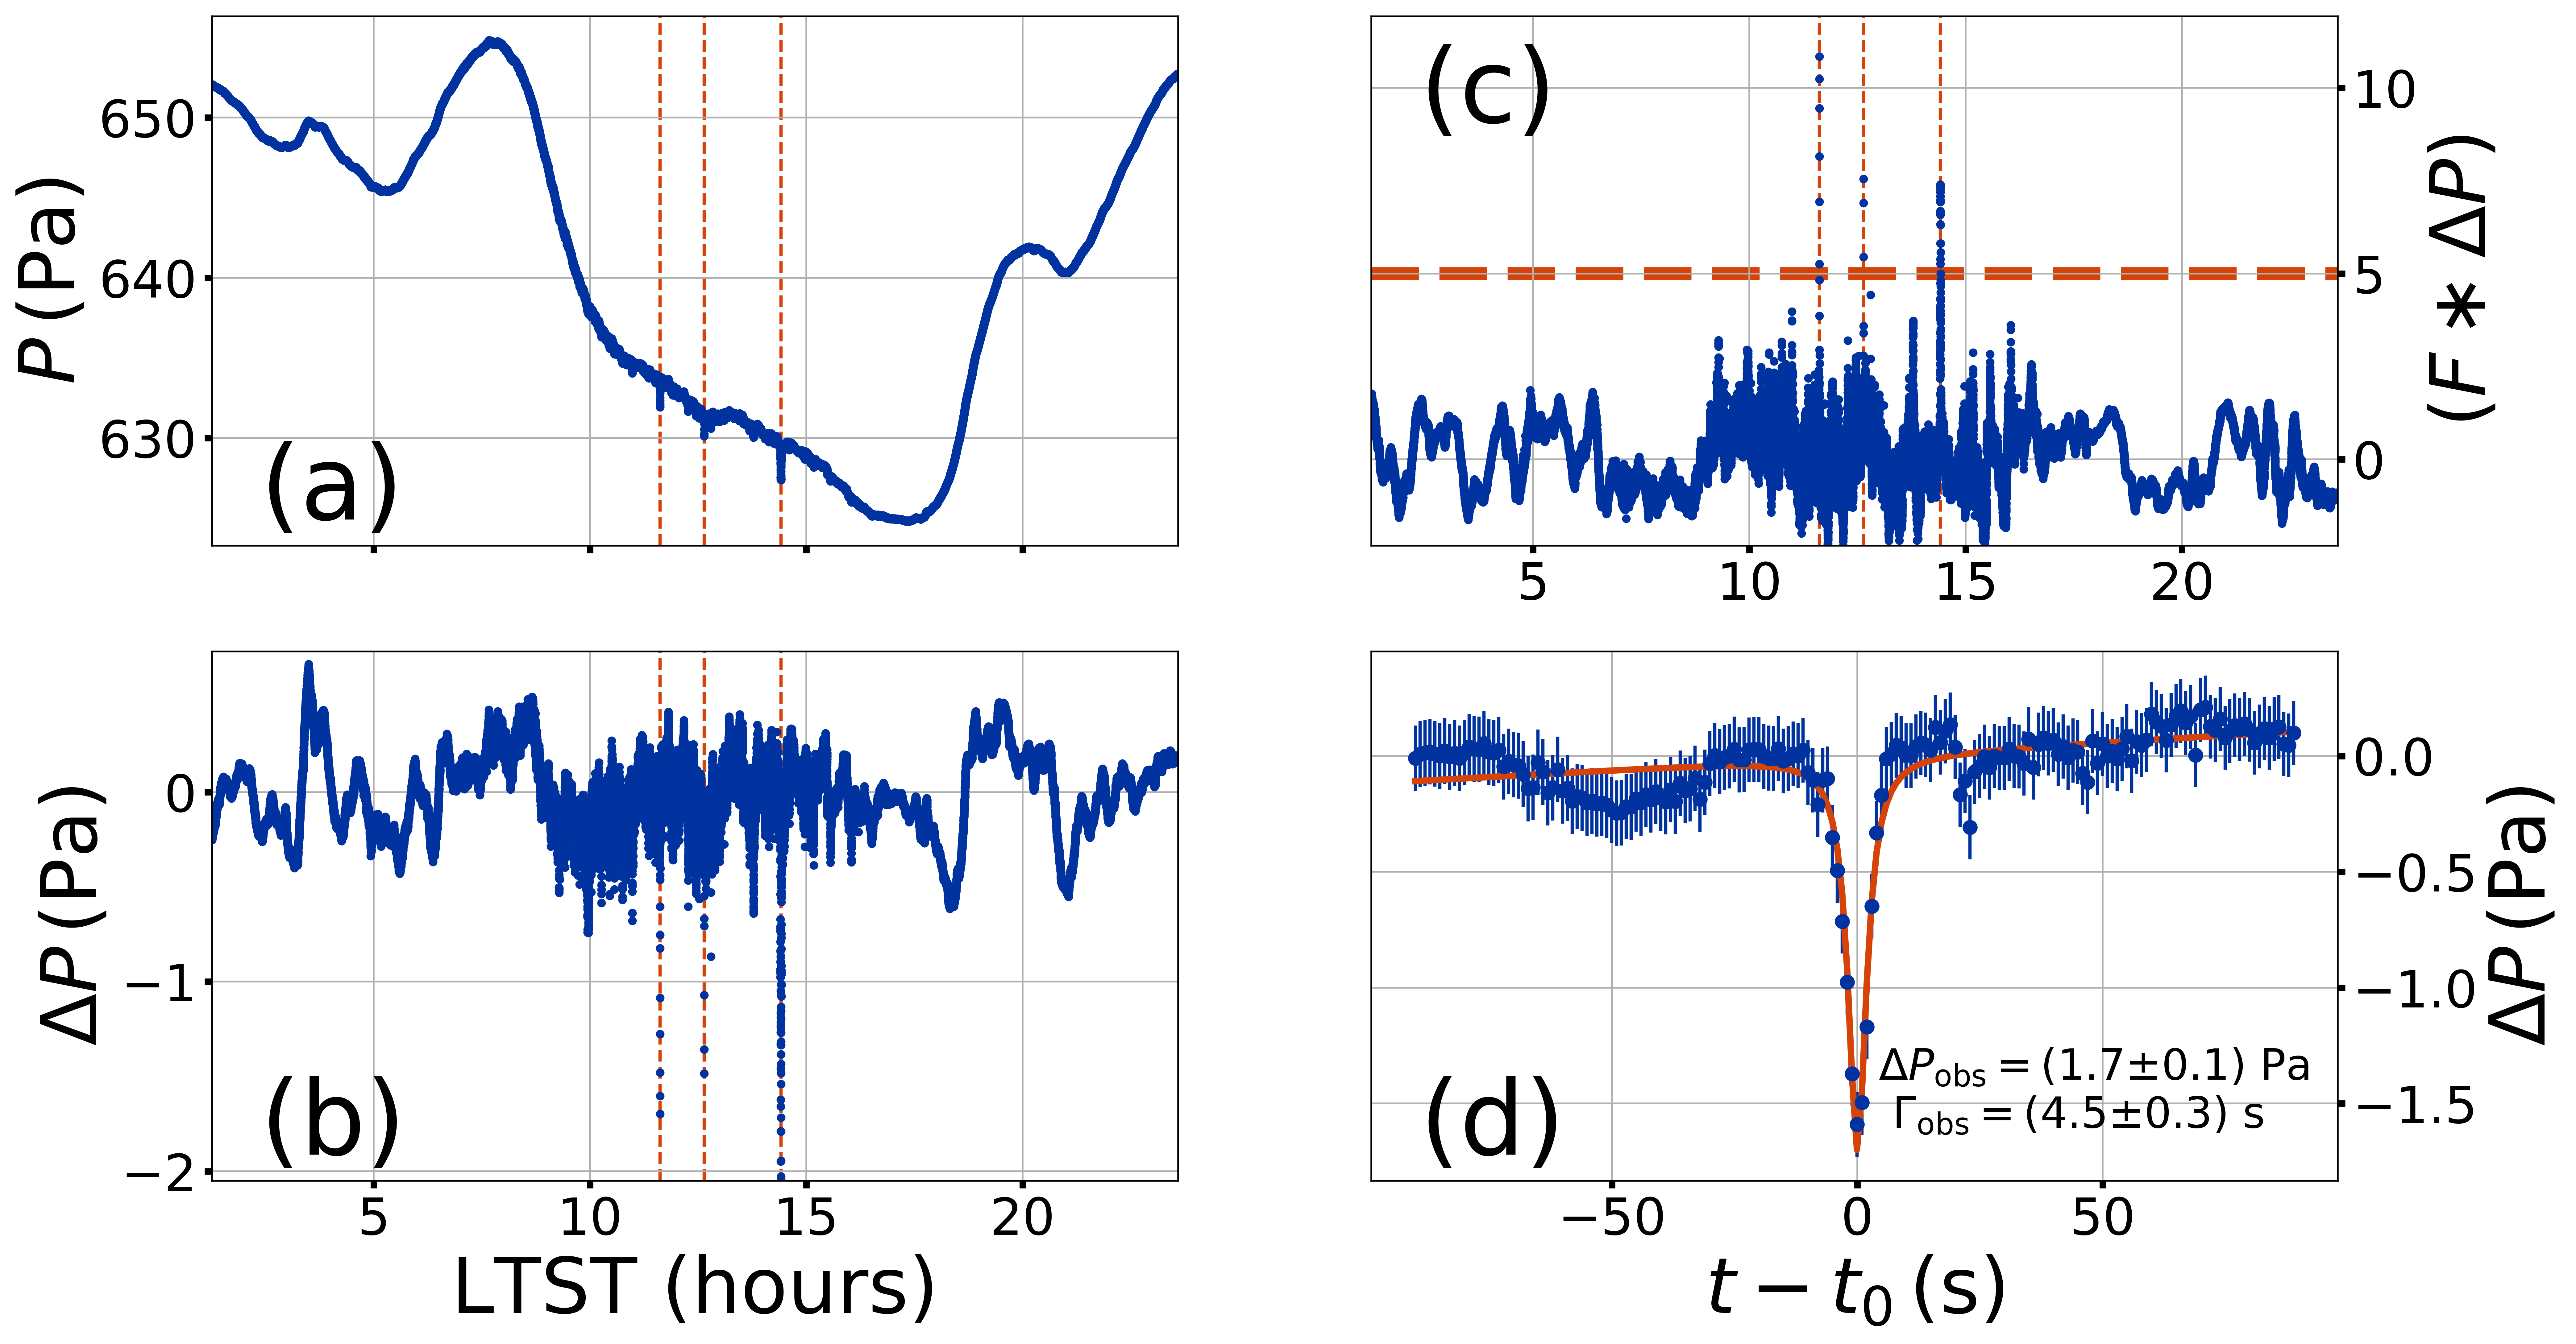
\includegraphics[width=\textwidth]{figures/data_conditioning_and_fit.png}
    \caption{(a) The pressure time-series for sol 392, as blue dots. The vertical orange lines highlight the detected vortex signals. (b) The time-series after application of the mean boxcar filter. Apparent by eye, the scatter in the time-series increases around mid-day. (c) Convolution of the matched filter with the time-series in (b). The horizontal dashed orange line shows the detection threshold of 5. (d) A model fit (solid orange line) to the deepest vortex discovered on sol 392, along with the model fit parameters -- each point's uncertainty is calculated via $1.4826\ \times$ the median absolute deviation in the window centered on that point.}
    \label{fig:data_conditioning_and_fit}
\end{figure}

\subsection{Fitting Wind Profiles}
\label{sec:Pressure and Wind Models}
To assess the intrinsic vortex properties and encounter geometries, we also fit wind speed profiles to the wind speed time-series that coincide in time with the peaks found by our search. The wind speed signal consists both of an ambient wind $U$ and the vortex wind $V(r)$, which is a function of radial distance (and therefore time). For the Rankine vortex model \citep{1991ExFl...11...73V}, $V(r)$ is given by
\begin{equation}
    V(r) = V_{\rm act} \frac{2 \left( \frac{r}{D_{\rm act}/2} \right) }{1 + \left( \frac{r}{D_{\rm act}/2} \right)^2},
\end{equation}
where $V_{\rm act}$ is the tangential wind speed at the vortex diameter. Similar to the pressure signal, a non-zero $b$ means the maximum wind speed encountered $V_{\rm obs}$ is less than the actual maximum at the vortex diameter. We model the observed vortex wind profile as
\begin{equation}
    V(t) = V_{\rm obs} \frac{\sqrt{1 + \left( U_1/b \right)^2 \left( t - t_0 \right)^2}}{1 + \left(\frac{t - t_0}{\Gamma_{\rm obs}/2}\right)^2},\label{eqn:wind_profile}
\end{equation}
where $U_1$ is the ambient wind speed before the encounter and which we take as the advective speed for the vortex. Strictly, this model breaks down for $b = 0$, but such an encounter is statistically unlikely \citep{2018Icar..299..166J}. Many of the wind signals exhibit a different ambient wind speed before the encounter ($U_1$) than after the encounter ($U_2$). Thus, the total wind speed observed $W(t)$ is the vector sum of the ambient wind and vortex wind, given by 
\begin{equation}
    W(t) = \left\{
    \begin{array}{ll}
            \sqrt{V^2 + 2 U_1 V \cos \theta + U_1^2}, & \left( t - t_0 \right) \leq 0\\
            \sqrt{V^2 + 2 U_2 V \cos \theta + U_2^2}, & \left( t - t_0 \right) > 0\\
    \end{array},\label{eqn:total_wind_speed}
\end{equation}
where $\cos \theta = b/\sqrt{b^2 + \left( U_{1/2} \right)^2\left( t - t_0 \right)^2}$. 

We fit the pressure and wind speed profiles for each encounter in two separate steps -- first, the pressure, then the wind speed. In so doing, we hold the $\Gamma_{\rm obs}$-value fixed from the pressure profile fit. Experimentation showed this approach most frequently gave reasonable results, and Figure \ref{fig:vortices_and_windspeed} shows several examples of the profile fits. 

As we show in Appendix \ref{sec:Inferring Encounter Geometries from the Pressure and Velocity Profiles}, we can estimate $\Delta P_{\rm act}$ and $V_{\rm act}$, along with the encounter distance $b$, from the observed parameters. To check this approach, we applied these models to many synthetic vortex encounters for a range of encounter geometries, vortex parameters, and time-series noise representative of the observed values. We found that, for encounters with $b \lesssim D_{\rm act}$, we were able to recover the assumed parameters to within 50\% for the majority of cases. For encounters farther than that, the signals were usually lost in the noise. We also required that the estimated $V_{\rm obs}$ exceed the scatter in the windspeed data $\sigma$ by a factor of five to ensure a robust detection. Future work should explore more robust approaches. In what follows, we initially retain all vortices detected, regardless of their best-fit $b$-values, since the best-fit $\Delta P_{\rm obs}$- and $\Gamma_{\rm obs}$ are independent of $b$, but for results later on that depend on $b$, we dropped those vortices with $b > D_{\rm act}$ and $V_{\rm obs}/\sigma < 5$, leaving \boverDactltone\ vortices. That transition is clearly indicated in the narrative below.

\begin{figure}
\centering
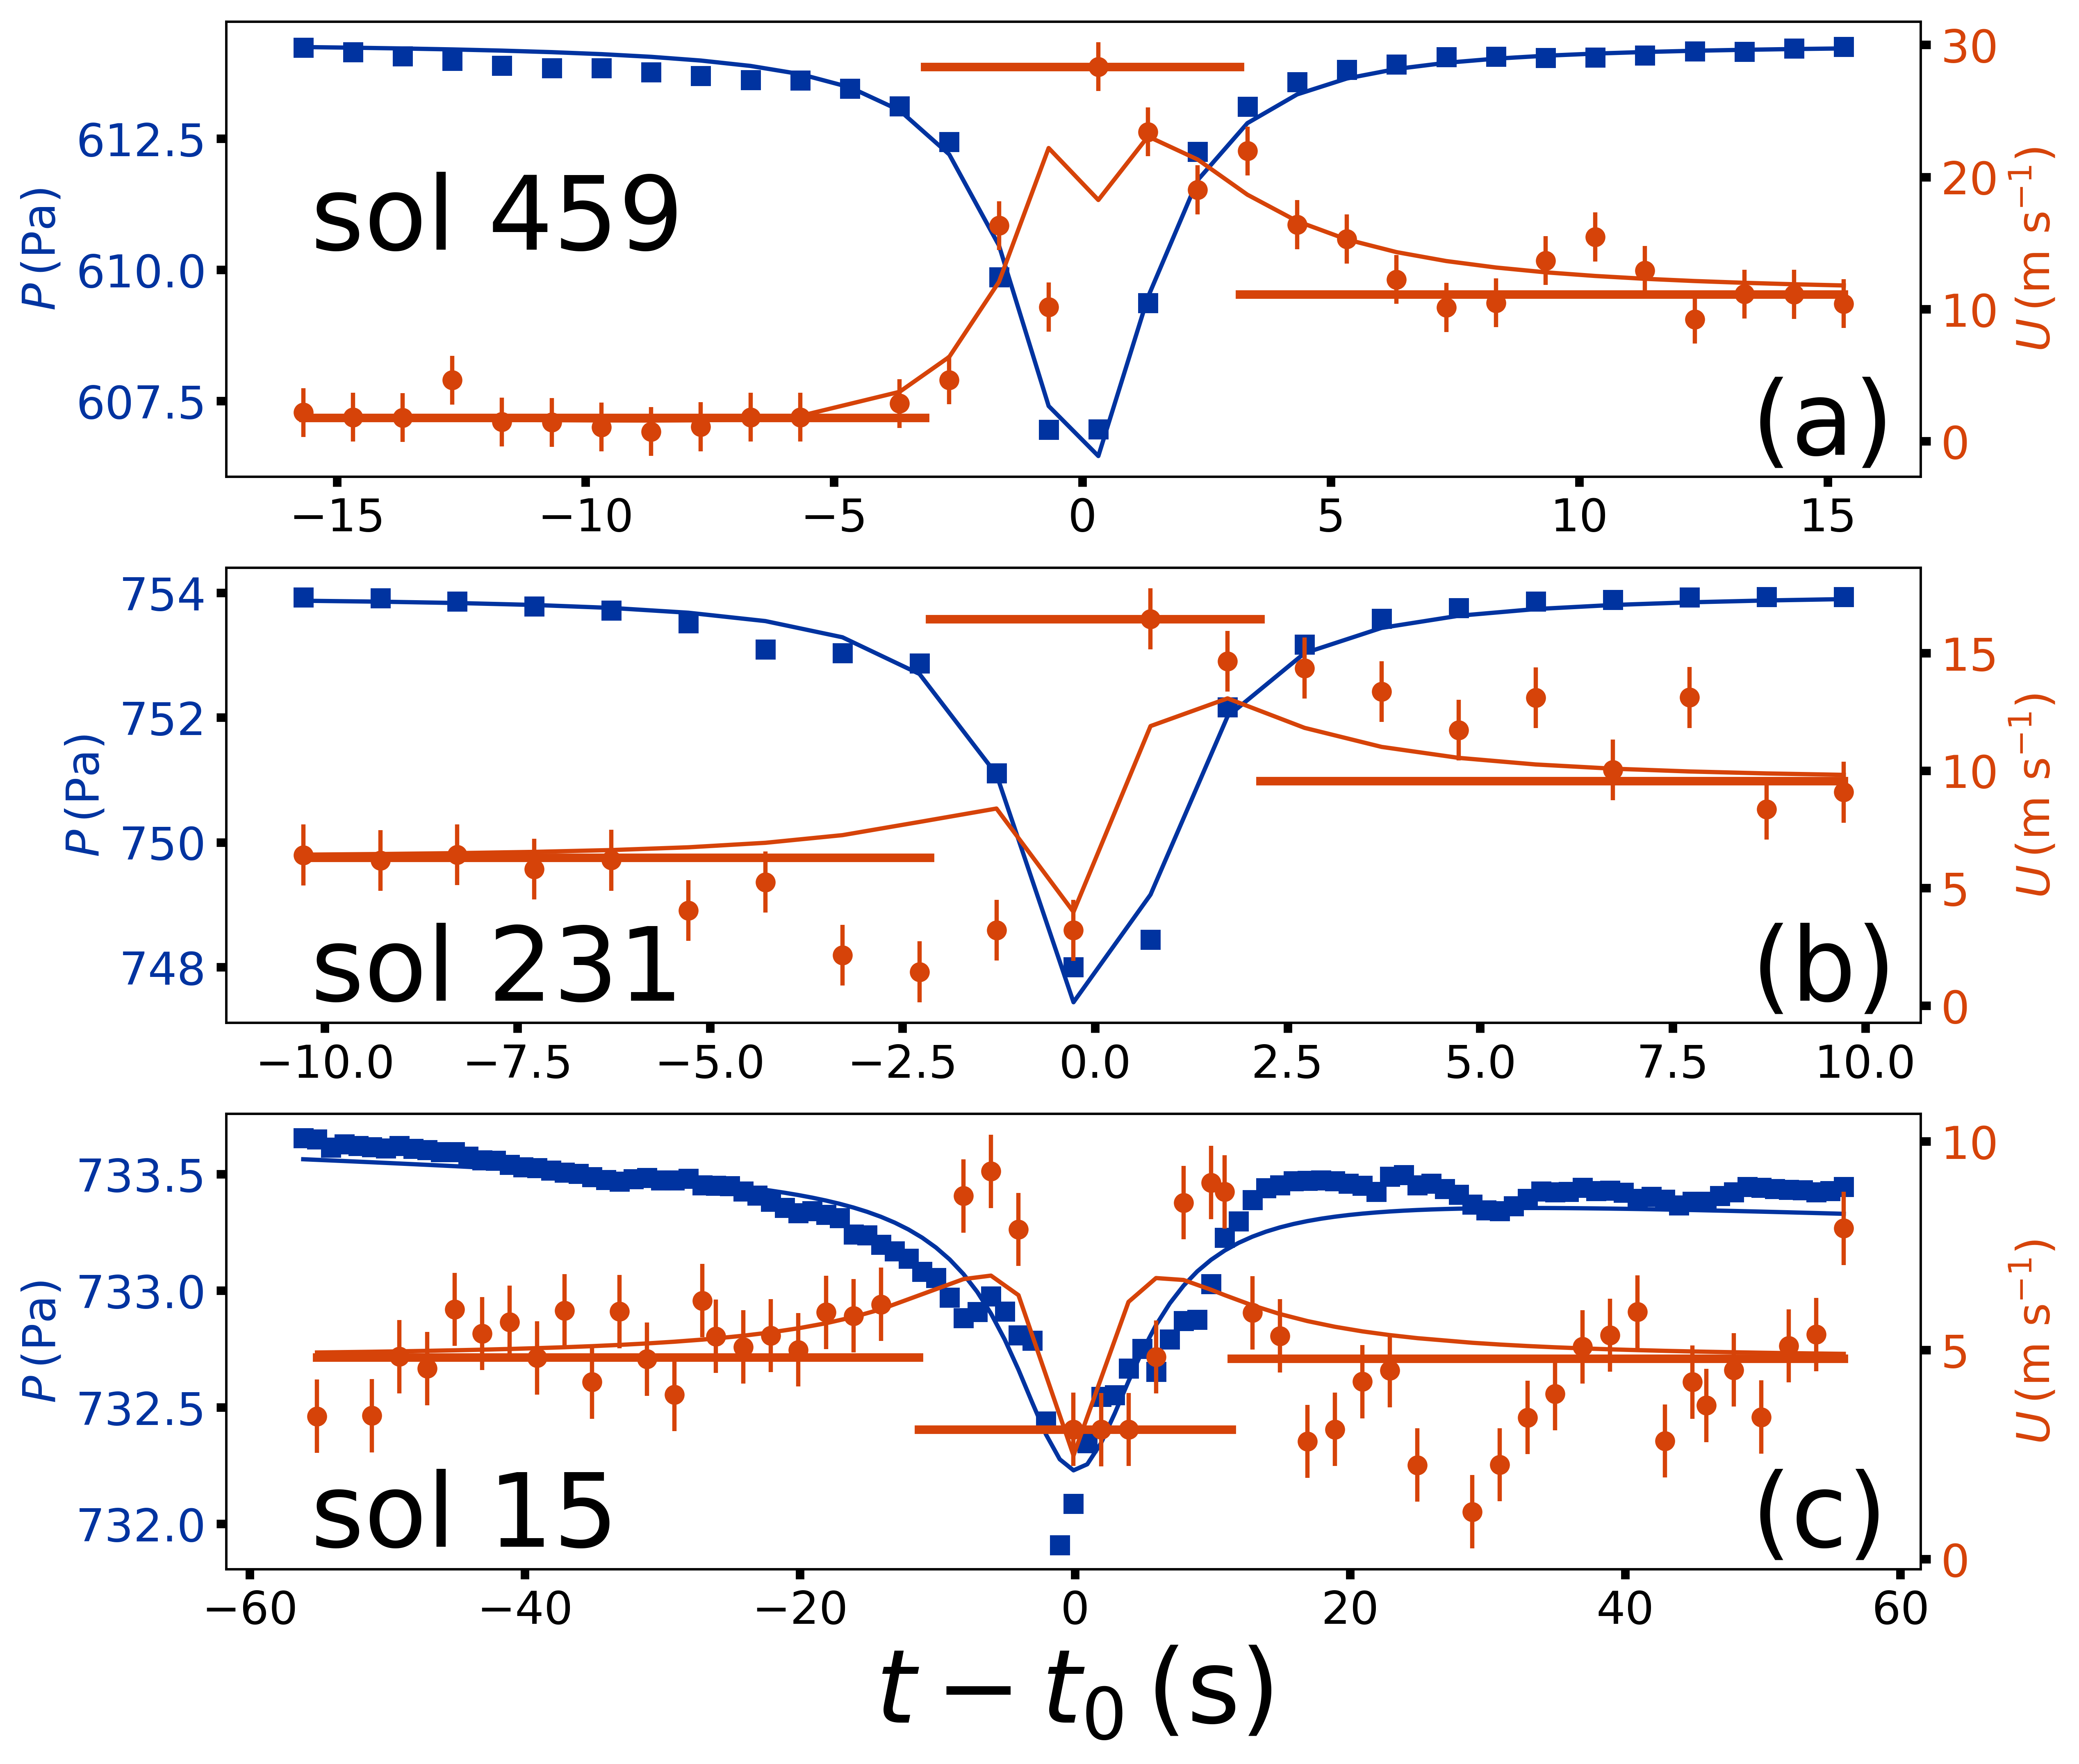
\includegraphics[width=0.48\textwidth]{figures/vortices_and_windspeed.png}
\caption{Pressure data (blue dots) and models (blue lines) and horizontal windspeed data (orange dots) and models. \label{fig:vortices_and_windspeed}}
\end{figure}

\subsection{Vortex Statistics}
\label{sec:Vortex Statistics}
Figure \ref{fig:DeltaPobs_vs_Gammaobs}(a) shows our collection of best-fit $\Gamma_{\rm obs}$- and $\Delta P_{\rm obs}$-values, along with their respective cumulative histograms. Inspecting an initial tranche of detections by-hand, we found that vortices with best-fit $\Gamma_{\rm obs} > 100\,{\rm s}$ and/or $\Delta P_{\rm obs} < 0.1\,{\rm Pa}$ tended not to resemble true vortices but instead appeared simply to be incoherent pressure excursions, so we dropped \maskedvortices\ of these initial detections, leaving the \totalvortices\ vortex signals depicted in Figure \ref{fig:DeltaPobs_vs_Gammaobs}. The largest $\Delta P_{\rm obs}$-value we found was \largestDeltaPobs\ on sol \largestDeltaPobssol, which seems to correspond to the deepest vortex reported in \citet{2020arXiv200501134S}. The longest-duration vortex occurred on sol \largestGammaobssol\ and lasted \largestGammaobs. The 50\% quantile values are $\Gamma_{\rm obs} = \left( 9.3 \pm 0.2 \right)\,{\rm s}$ and $\Delta P_{\rm obs} = \left( 1.13 \pm 0.03 \right)\,{\rm Pa}$ (indicated by the dashed, orange lines in Figure \ref{fig:DeltaPobs_vs_Gammaobs}). As evident in previous analyses of Mars lander pressure time-series \citep[e.g.,][]{2010JGRE..115.0E16E}, there is a marked absence of long-duration/deep (i.e., large $\Delta P_{\rm obs}$) vortices. This absence simply reflects the miss distance effect: most encounters between the barometer and vortex occur some distance from the vortex center ($b > 0$ as in Equation \ref{eqn:radial_distance}), where the pressure profile is more shallow and of longer duration \citep{2018Icar..299..166J}.

The flattening of the cumulative histogram for $\Delta P_{\rm obs}$ (Figure \ref{fig:DeltaPobs_vs_Gammaobs}c) near $1.1\,{\rm Pa}$ indicates a decline in the number of detected vortices below that value. This decline occurs, at least in part, because of difficulty detecting these more shallow signals against noise \citep{2018Icar..299..166J}. Given the possible strong dependence of dust-lifting on $\Delta P$, the exact form of the histogram of $\Delta P_{\rm obs}$-values is critical for evaluating the population's atmospheric influence. We fit a power-law to the cumulative histogram with an exponent $\gamma = -2.39\pm0.02$, which indicates the differential histogram has an exponent $\approx -3.39$. This exponent is consistent with the value reported in \citet{2020arXiv200501134S} for the same dataset and with the value reported in \citet{2018Icar..299..166J} for the vortices detected by the Phoenix Mission. (On a related note, since the best-fit exponent for a differential histogram can depend on the chosen binning, we suggest such analyses use cumulative histograms or a data-informed scheme for binning -- \citealp{2016SSRv..203..277L}.)

\begin{figure}
    \centering
    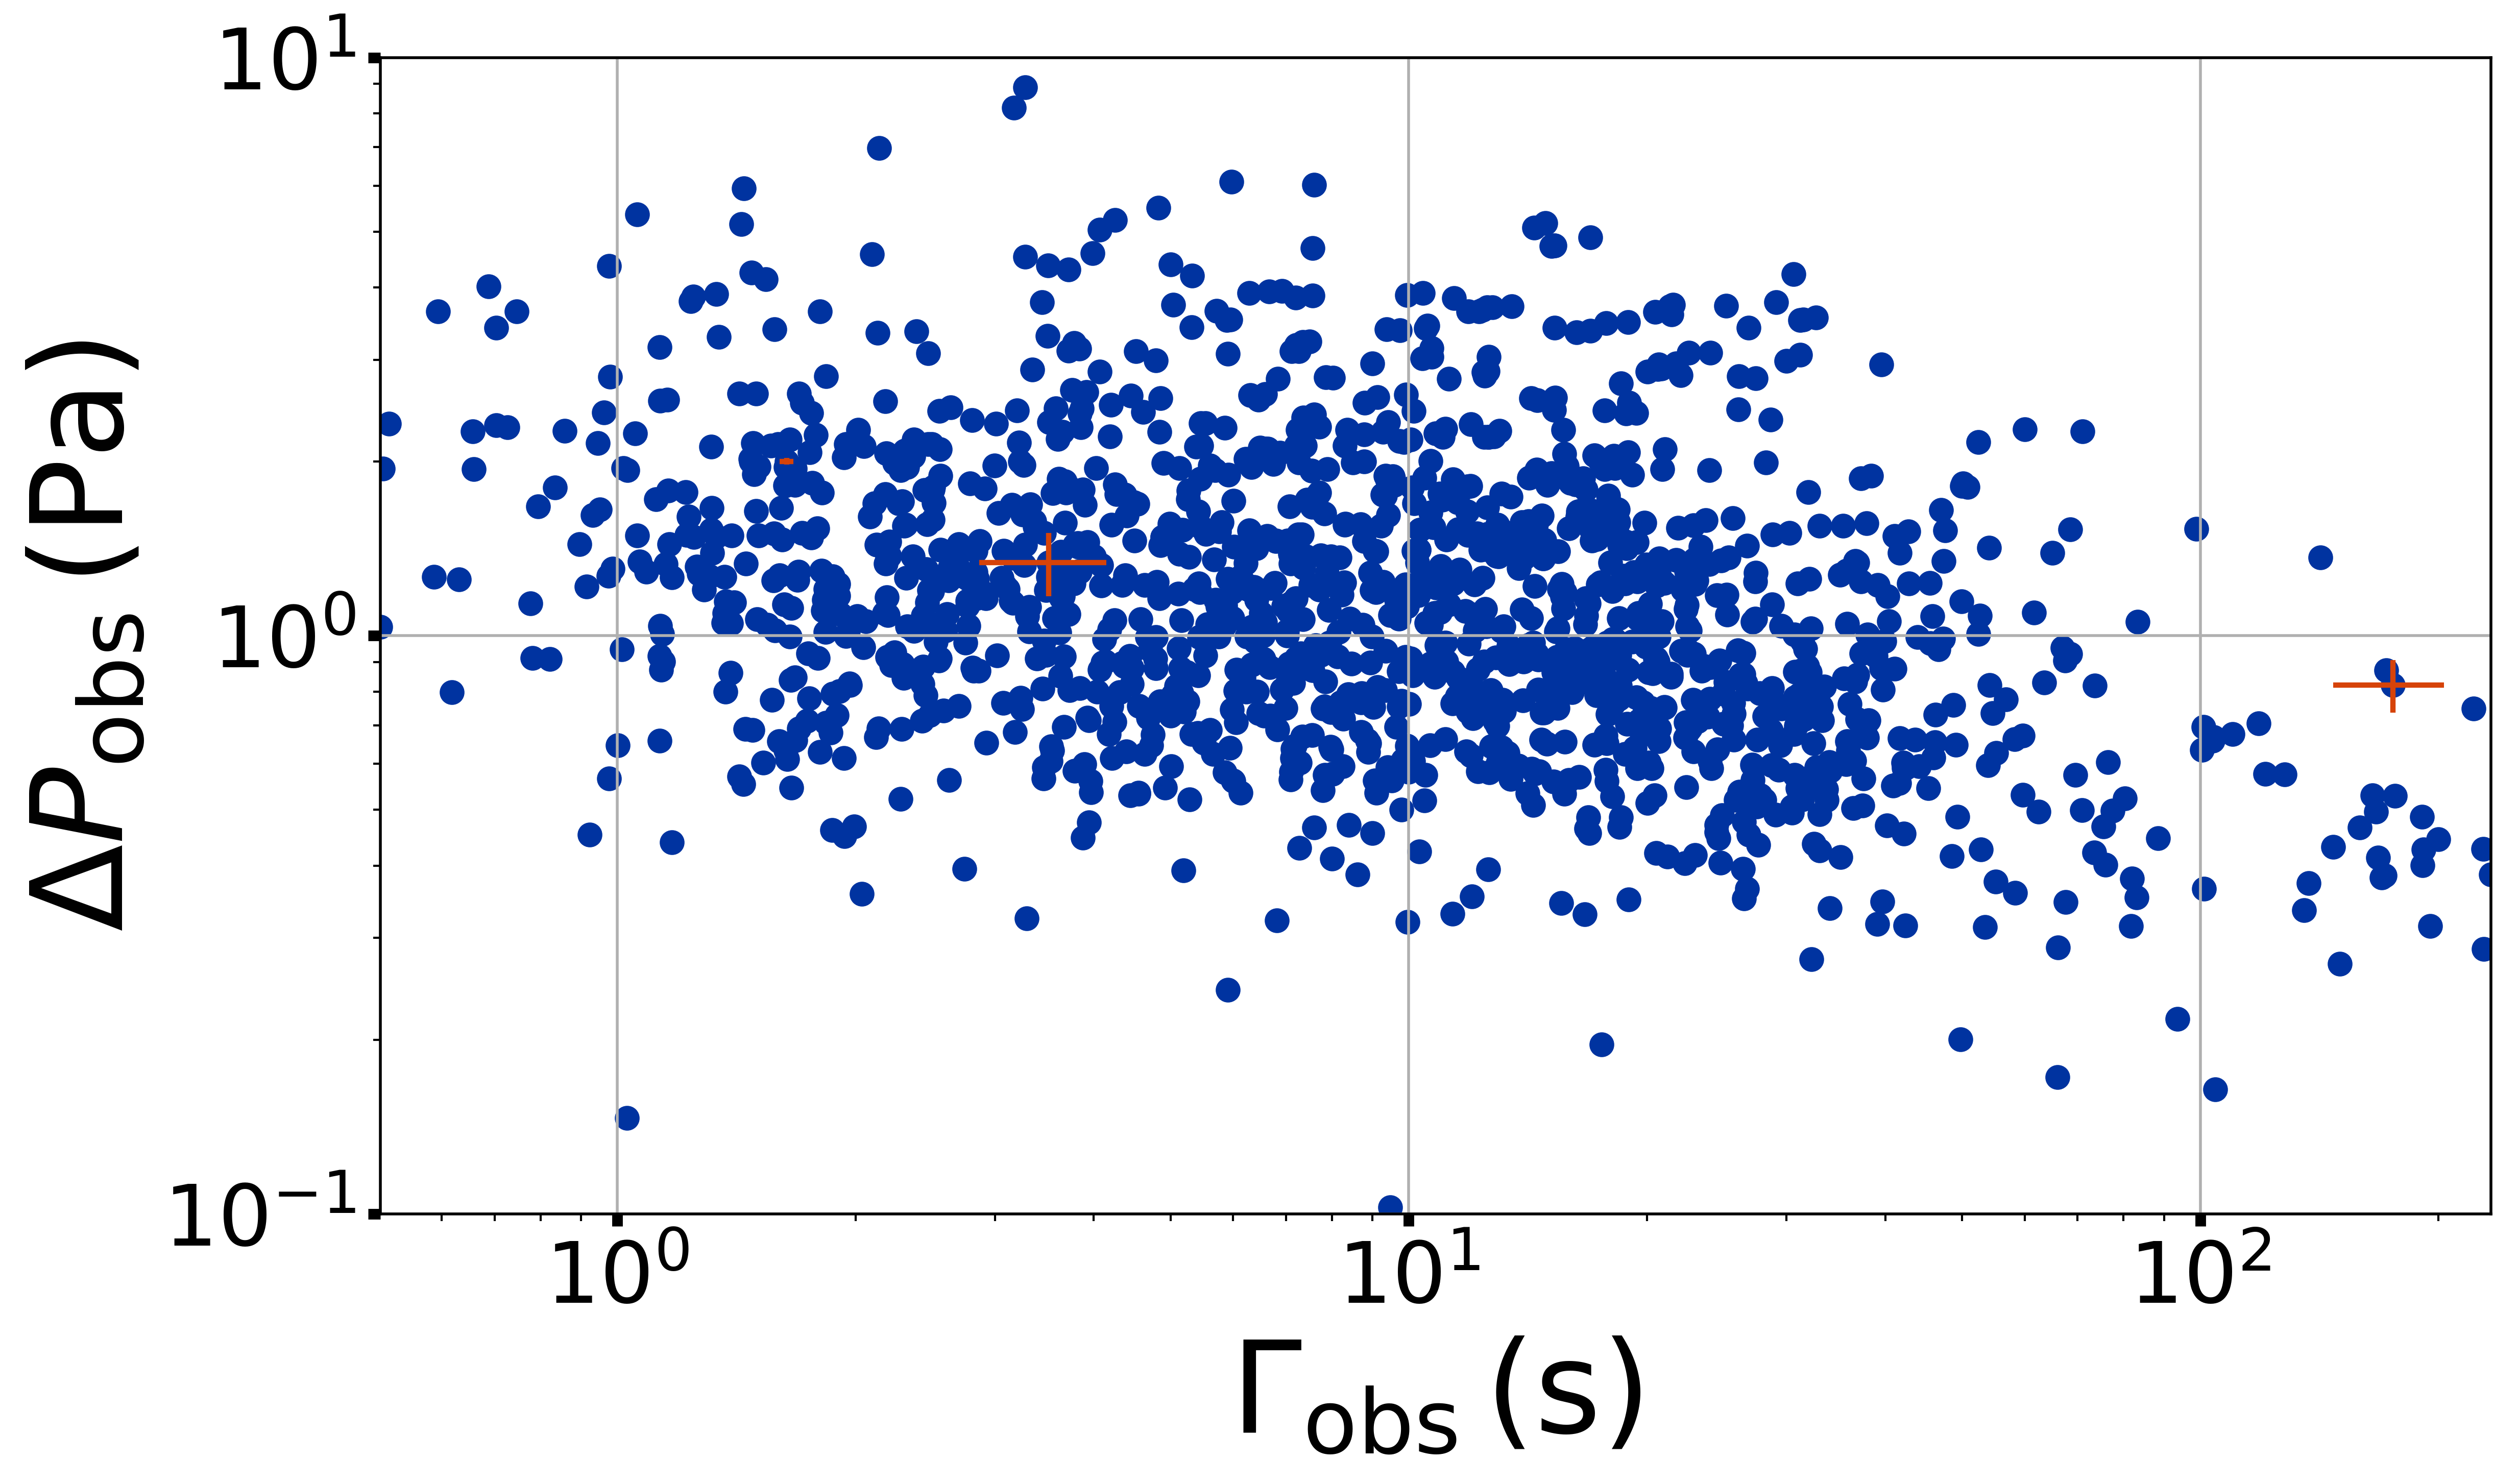
\includegraphics[width=\textwidth]{figures/DeltaPobs_vs_Gammaobs.png}
    \caption{(a) The best-fit $\Delta P_{\rm obs}$- and $\Gamma_{\rm obs}$-values (blue dots). Representative error bars are shown as orange crosses. (b) Cumulative histogram of $\Gamma_{\rm obs}$-values, along with the 50\% quantile value ($\Gamma_{\rm obs} = \left( 9.3 \pm 0.2 \right)\,{\rm s}$) shown by the dashed, orange line. (c) Cumulative histogram of $\Delta P_{\rm obs}$-values, along with the 50\% quantile value ($\Delta P_{\rm obs} = \left( 1.13 \pm 0.03 \right)\,{\rm Pa}$) shown by the dashed, orange line. The dash-dotted green line shows a power-law fit to the histogram, with $N \propto \Delta P_{\rm obs}^{-2.45\pm0.02}$.}
    \label{fig:DeltaPobs_vs_Gammaobs}
\end{figure}

\begin{figure}
    \centering
    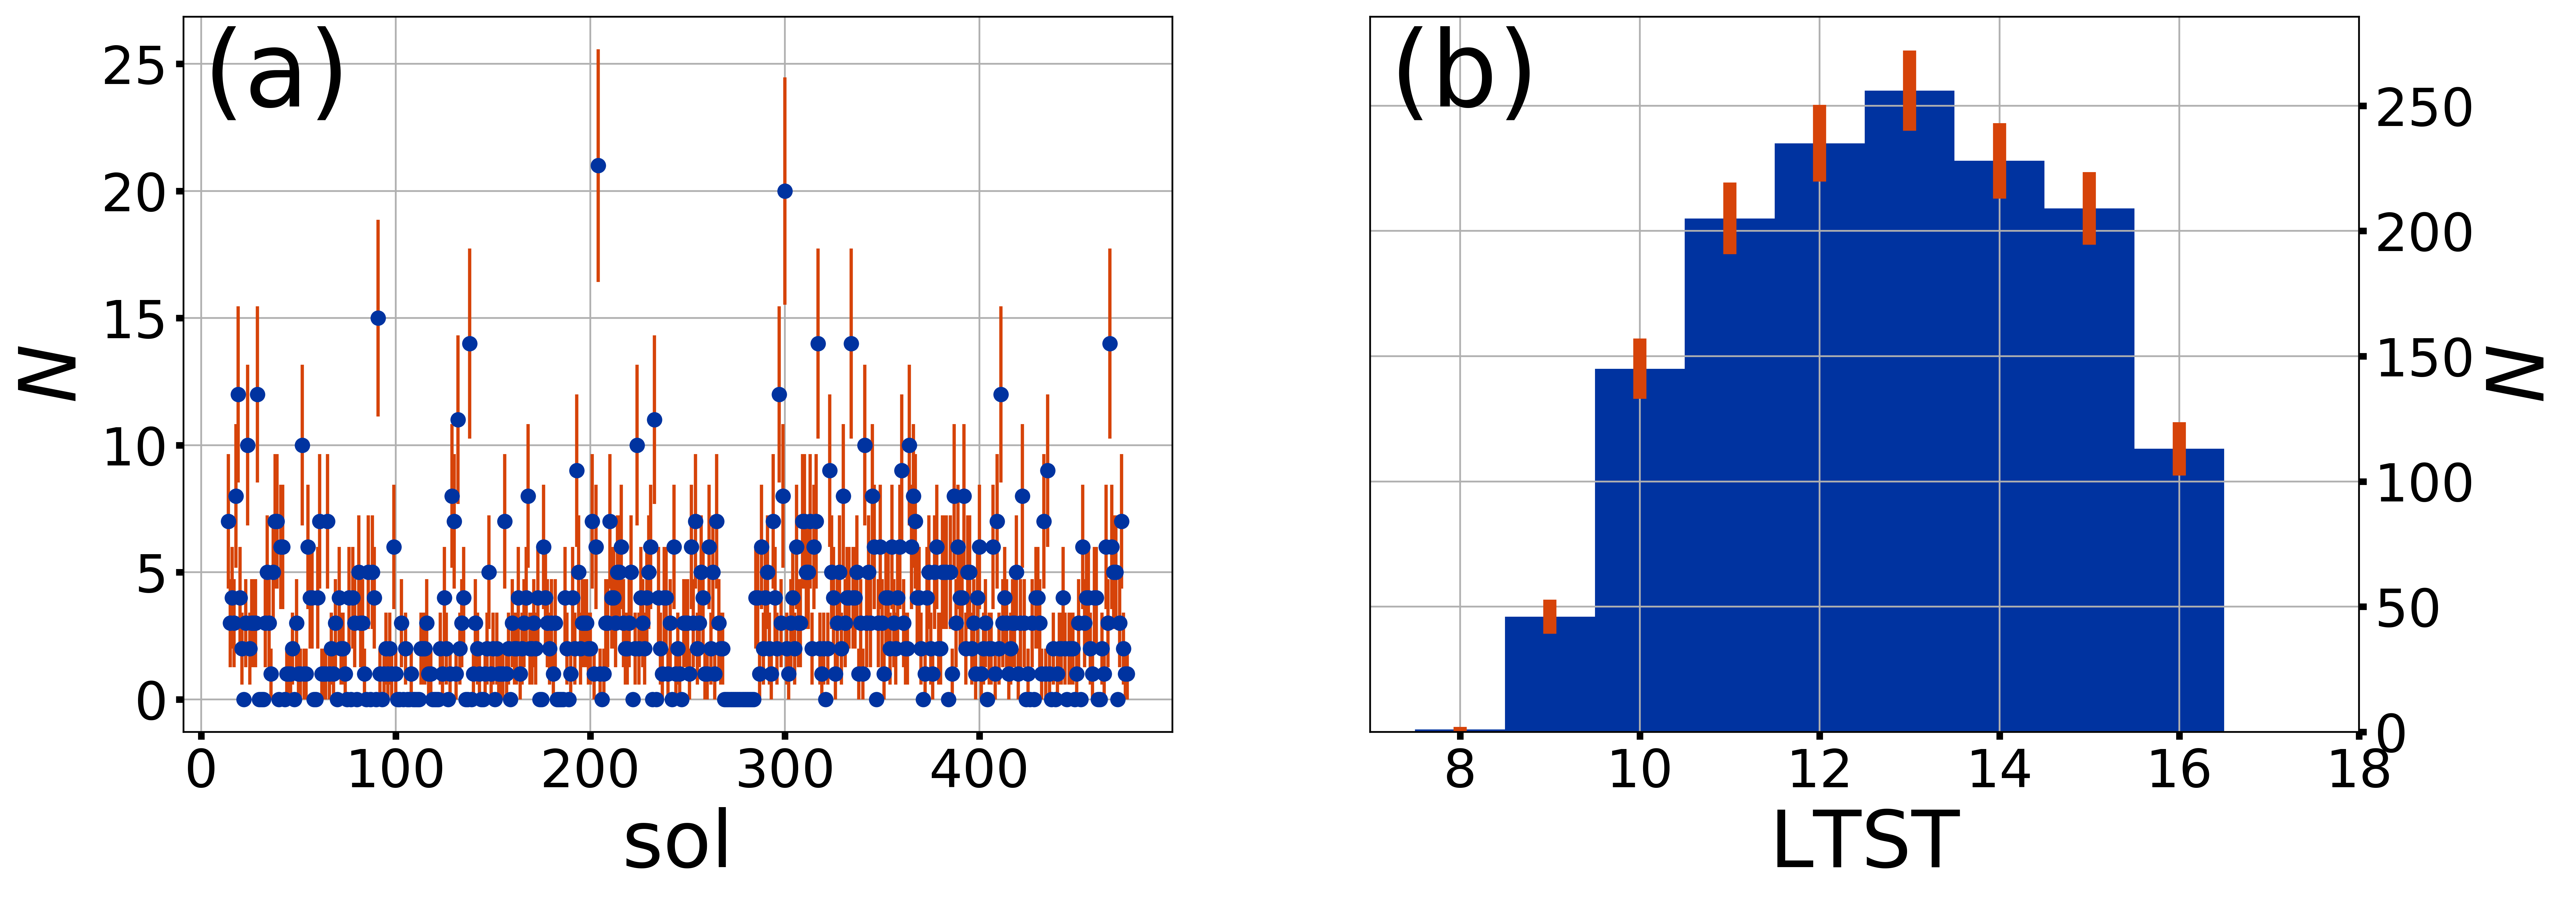
\includegraphics[width=\textwidth]{figures/sol_and_t0_histograms.png}
    \caption{(a) The number of vortices during each sol $N$ (blue dots) along with the values for $L_{\rm s}$ (dashed, grey lines). (Northern spring starts at $L_{\rm s} = 90^\circ$.) The orange histogram shows the number of vortices per sol for bins 35 sols wide. (b) The number of vortices per hour of local true solar time (LTST). Orange lines in both panels show Poisson error bars.}
    \label{fig:sol_and_t0_histograms}
\end{figure}

The vortices also exhibit sol-to-sol and hour-to-hour variation, as illustrated in Figure \ref{fig:sol_and_t0_histograms}. Panel (a) shows that the maximum daily of vortices occurred on sol 204 of the mission, in the middle of northern spring, while the next maximum occurs on sol 300, near the beginning of northern summer. Although \citet{2020arXiv200501134S} used a different procedure, that study found a broadly similar pattern -- a dip in the occurrence rate centered on sol 100, with an increase going into sol 200 and beyond. Regarding the hour-to-hour variations, panel (b) shows that the maximum occurs between 12:00 and 13:00 LTST, with a nearly symmetric decline to either side. For this calculation, we totaled up the number of hours (and fractions thereof) during which pressure time-series were reported and then divided the number of vortices encountered during each of those hours over all sols by that total. These results contrast somewhat with those of \citet{2020arXiv200501134S}, which found a peak in vortex occurrence between 11:00 and 12:00 LTST. 

The $\Gamma_{\rm obs}$- and $\Delta P_{\rm obs}$-values exhibit intriguing trends as well. Figure \ref{fig:Gammaobs_DeltaPobs_vs_TOD_and_sol}(c) shows that, binned by the hour, the median value of $\Gamma_{\rm obs}$ increases from $2$ to $20\,{\rm s}$ from early morning to late afternoon. Figure \ref{fig:Gammaobs_DeltaPobs_vs_TOD_and_sol}(d) shows that median value for $\Delta P_{\rm obs}$ peaks around 12:00 LTST at $\left( 1.3\pm0.05 \right)\,{\rm Pa}$ with minimum values at either end of about $\left( 0.7\pm 0.1 \right)\,{\rm Pa}$ (where the uncertainties come from the error of the median in the corresponding bin). The values binned by sol (Figures \ref{fig:Gammaobs_DeltaPobs_vs_TOD_and_sol}a and b) show no obvious trends. 

\begin{figure}
    \centering
    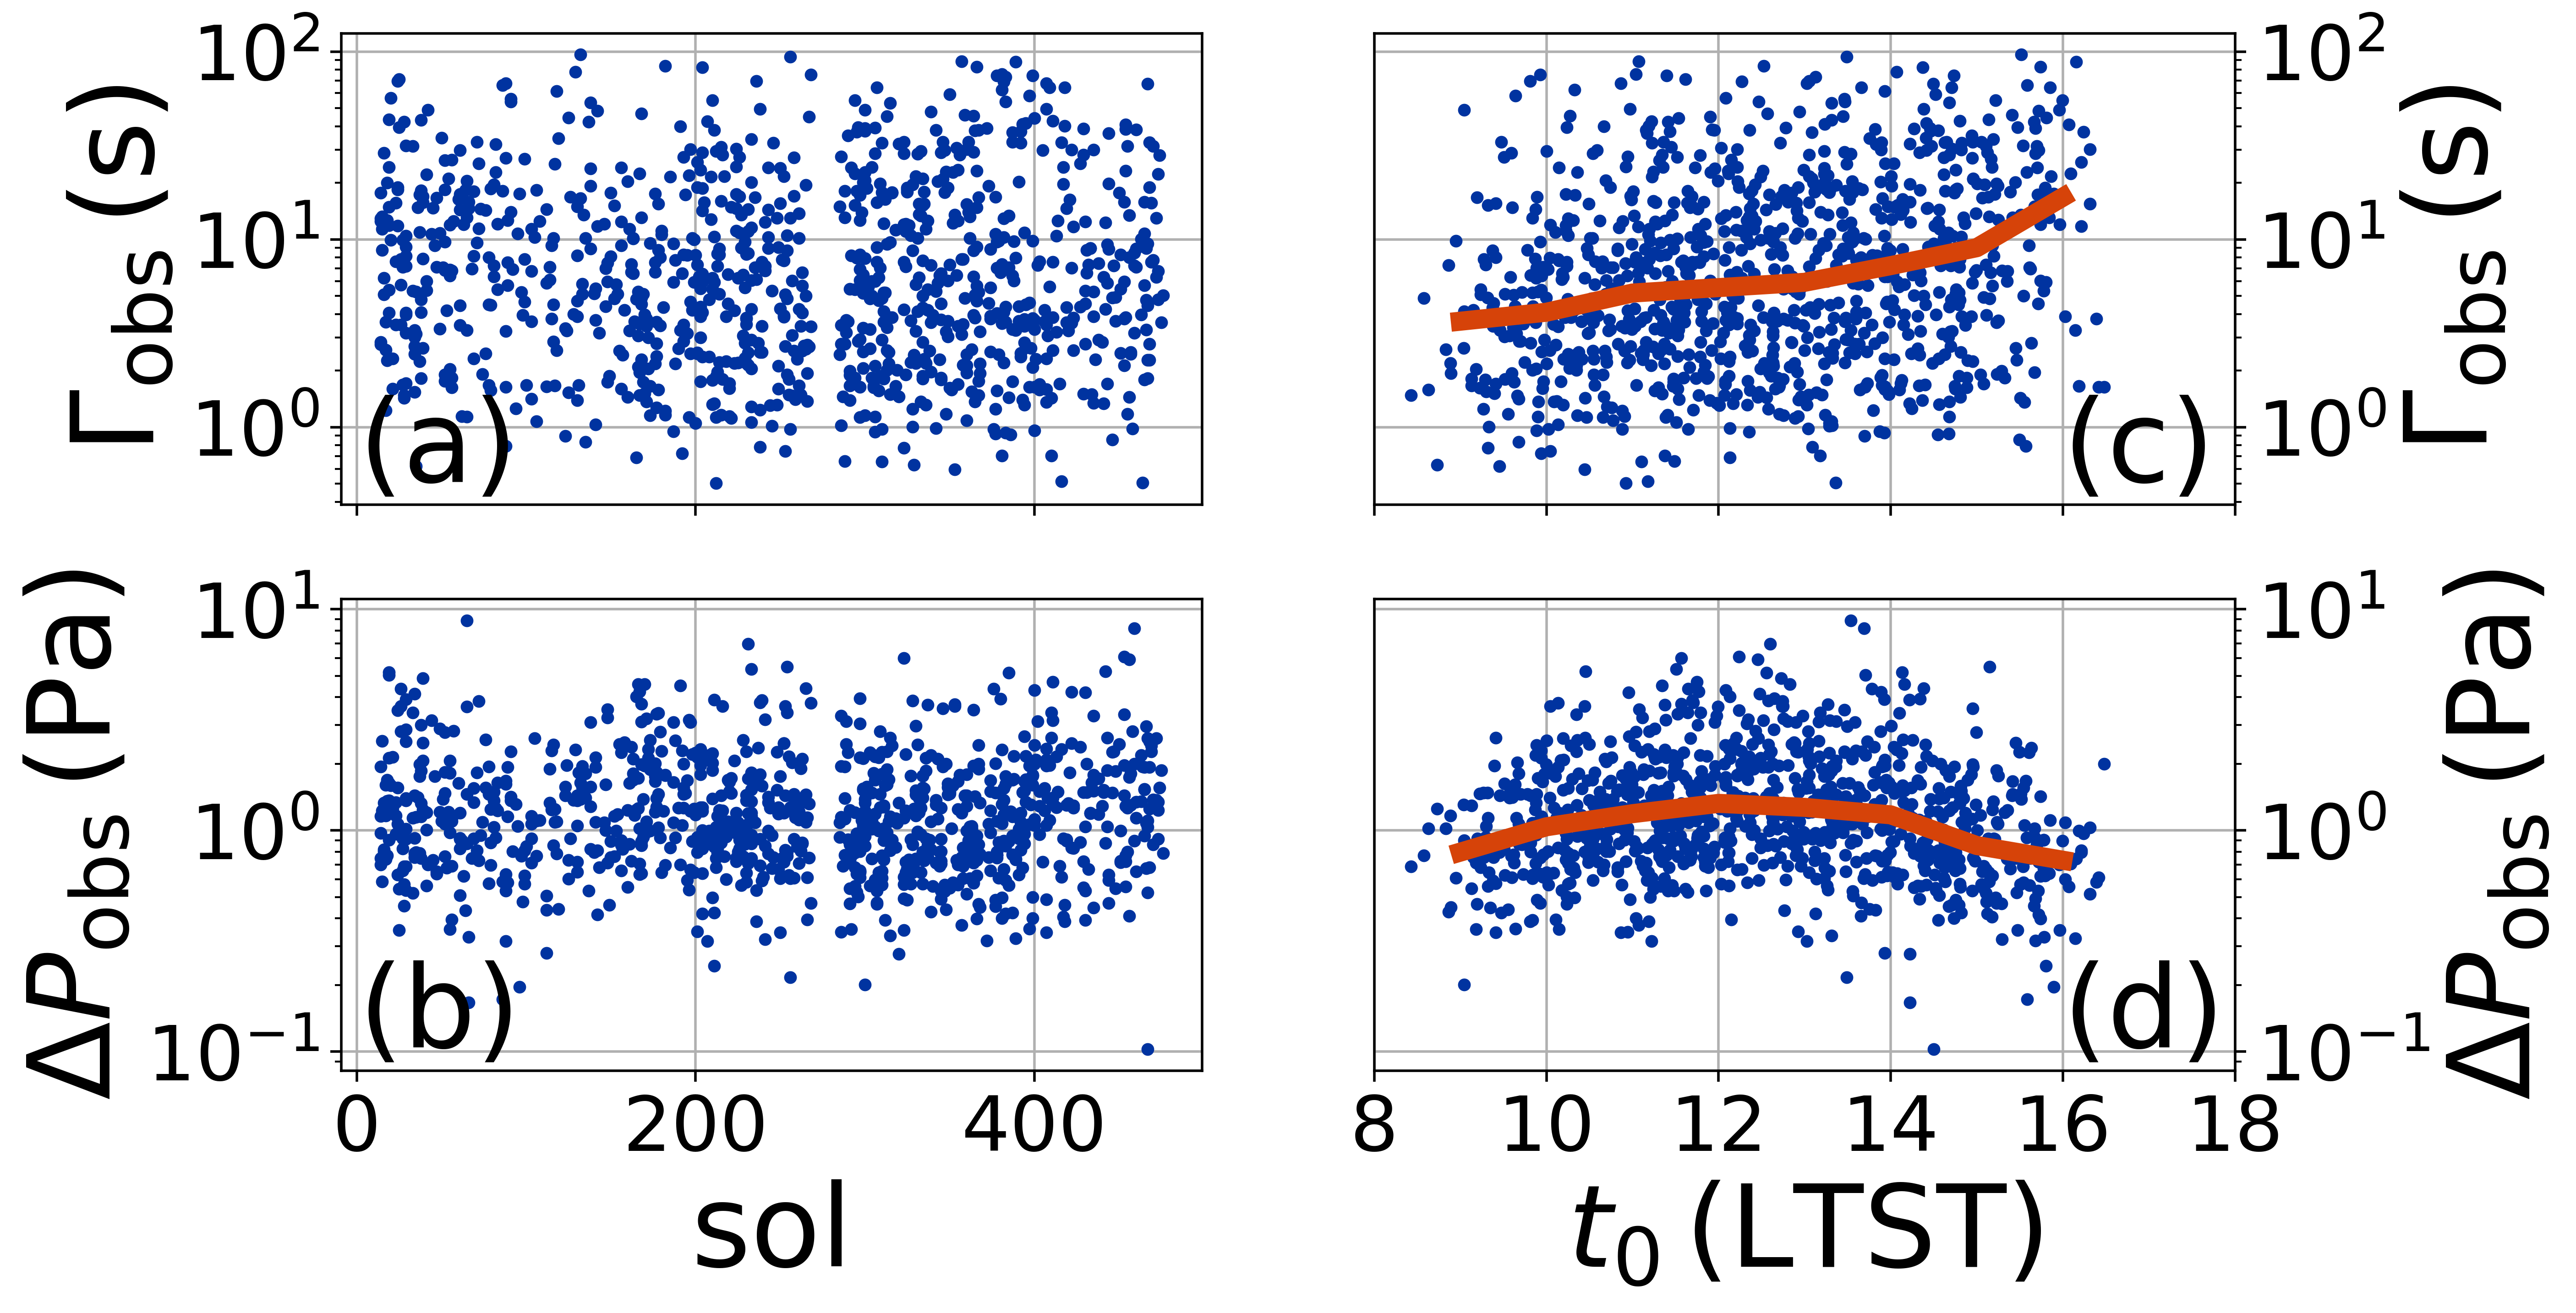
\includegraphics[width=\textwidth]{figures/Gammaobs_DeltaPobs_vs_TOD_and_sol.png}
    \caption{(a)/(b) Distributions of $\Gamma_{\rm obs}$ and $\Delta P_{\rm obs}$ by sol. (c)/(d) Distributions of $\Gamma_{\rm obs}$ and $\Delta P_{\rm obs}$ by time-of-day $t_0$. The orange lines show the distributions binned by hour.}
    \label{fig:Gammaobs_DeltaPobs_vs_TOD_and_sol}
\end{figure}

Presumably, these hour-to-hour trends reflect the influence of variable ambient conditions, but these data alone are not sufficient to judge what influence: the increase in $\Gamma_{\rm obs}$ could result either from intrinsically larger vortices late in the day or lower wind speeds $U$ advecting the same size vortices past the sensor. Fortunately, the TWINS wind speed data can shed light on this issue. Figure \ref{fig:vortices_and_windspeed} shows the three vortices with the largest $\Delta P_{\rm obs}$-values. We estimated the advection speed by taking the median value $U$ between 5- and 3-$\Gamma_{\rm obs}$ before the encounter time $t_0$. This approach returns a wind speed close enough in time to be a plausible estimate of the advection speed but early enough that the vortex did not significantly influence the measurement. 

Figure \ref{fig:U_vs_t0-sol_hist} shows the distribution of advective wind speeds associated with the observed vortices; the maximum, median, and minimum values are $19.1\pm2.3$, $7.6\pm1.0$, and $0.5\pm0.2 \,{\rm m\ s^{-1}}$, respectively. Panel (a) shows a clear decrease in wind speed during the lull in vortex encounters around sol 100 and an increase in wind speeds, along with a widened scatter, during the peak around sol 300. Panel (b) shows a small increase the median advective speed from the early to mid-morning (11:00) and then a steady decline of about 30\% thereafter. This decline in advection speed correlates very closely with the increase in $\Gamma_{\rm obs}$ from 11:00 to 16:00 LTST. Assuming uniformly distributed random encounter distances $b$, we expect the vortex duration to scale inversely with advection speed. Consequently, the increase in $\Gamma_{\rm obs}$ seen in Figure \ref{fig:Gammaobs_DeltaPobs_vs_TOD_and_sol}(c) seems likely to result from the decrease in advection speed, not from a systematic increase in vortex diameter. Indeed, the decline in $\Delta P_{\rm obs}$ seen in the afternoon comports with this result \citep{2020Icar..33813523J}.

% Figure \ref{fig:Dobs_vs_Gammaobs-DeltaPobs_hist} shows the distribution of $D_{\rm obs}$-values against $\Gamma_{\rm obs}$ and $\Delta P_{\rm obs}$, as well as a cumulative histogram. The maximum, minimum, and median values are $1100 \pm 240$, $75 \pm 21$, and $4 \pm 1 \,{\rm m}$, respectively. Not surprisingly, the $D_{\rm obs}$-values correlate positively with $\Gamma_{\rm obs}$ with scatter resulting from the relatively narrow range of advective wind speeds. 
% On the other hand, $D_{\rm obs}$ seems negatively correlated with $P_{\rm obs}$, and a power-law fit using the Levenberg-Marquardt algorithm \citep{Press2007} gives $D_{\rm obs} \propto \Delta P_{\rm obs}^{-0.42\pm0.04}$, where uncertainties come from the covariance matrix. As explained in \citet{2018Icar..299..166J}, for a vortex encounter with any miss distance $b$, we expect $\Delta P_{\rm obs}$ and $D_{\rm obs}$ are related to the vortex's central pressure excursion $\Delta P_{\rm act}$ and diameter $D_{\rm act}$ as $\Delta P_{\rm obs} D_{\rm obs}^2 = \Delta P_{\rm act} D_{\rm act}^2$. Figure \ref{fig:Dobs_vs_Gammaobs-DeltaPobs_hist}(b) could be interpreted, then, as encounters with vortices at a variety of miss distances but all with the same $\Delta P_{\rm act}$- and $D_{\rm act}$-values (the exponent $0.4\pm0.04$ diverges from 0.5 by less than $3\sigma$). However, such a result is totally unexpected as dust devil diameters are known to span a wide range and would be inconsistent with a variety of studies \citep[cf.][]{2016SSRv..203..277L}. Instead, this result probably only indicates that the range of miss distances plays an important role in setting the observed distribution. 

\begin{figure}
    \centering
    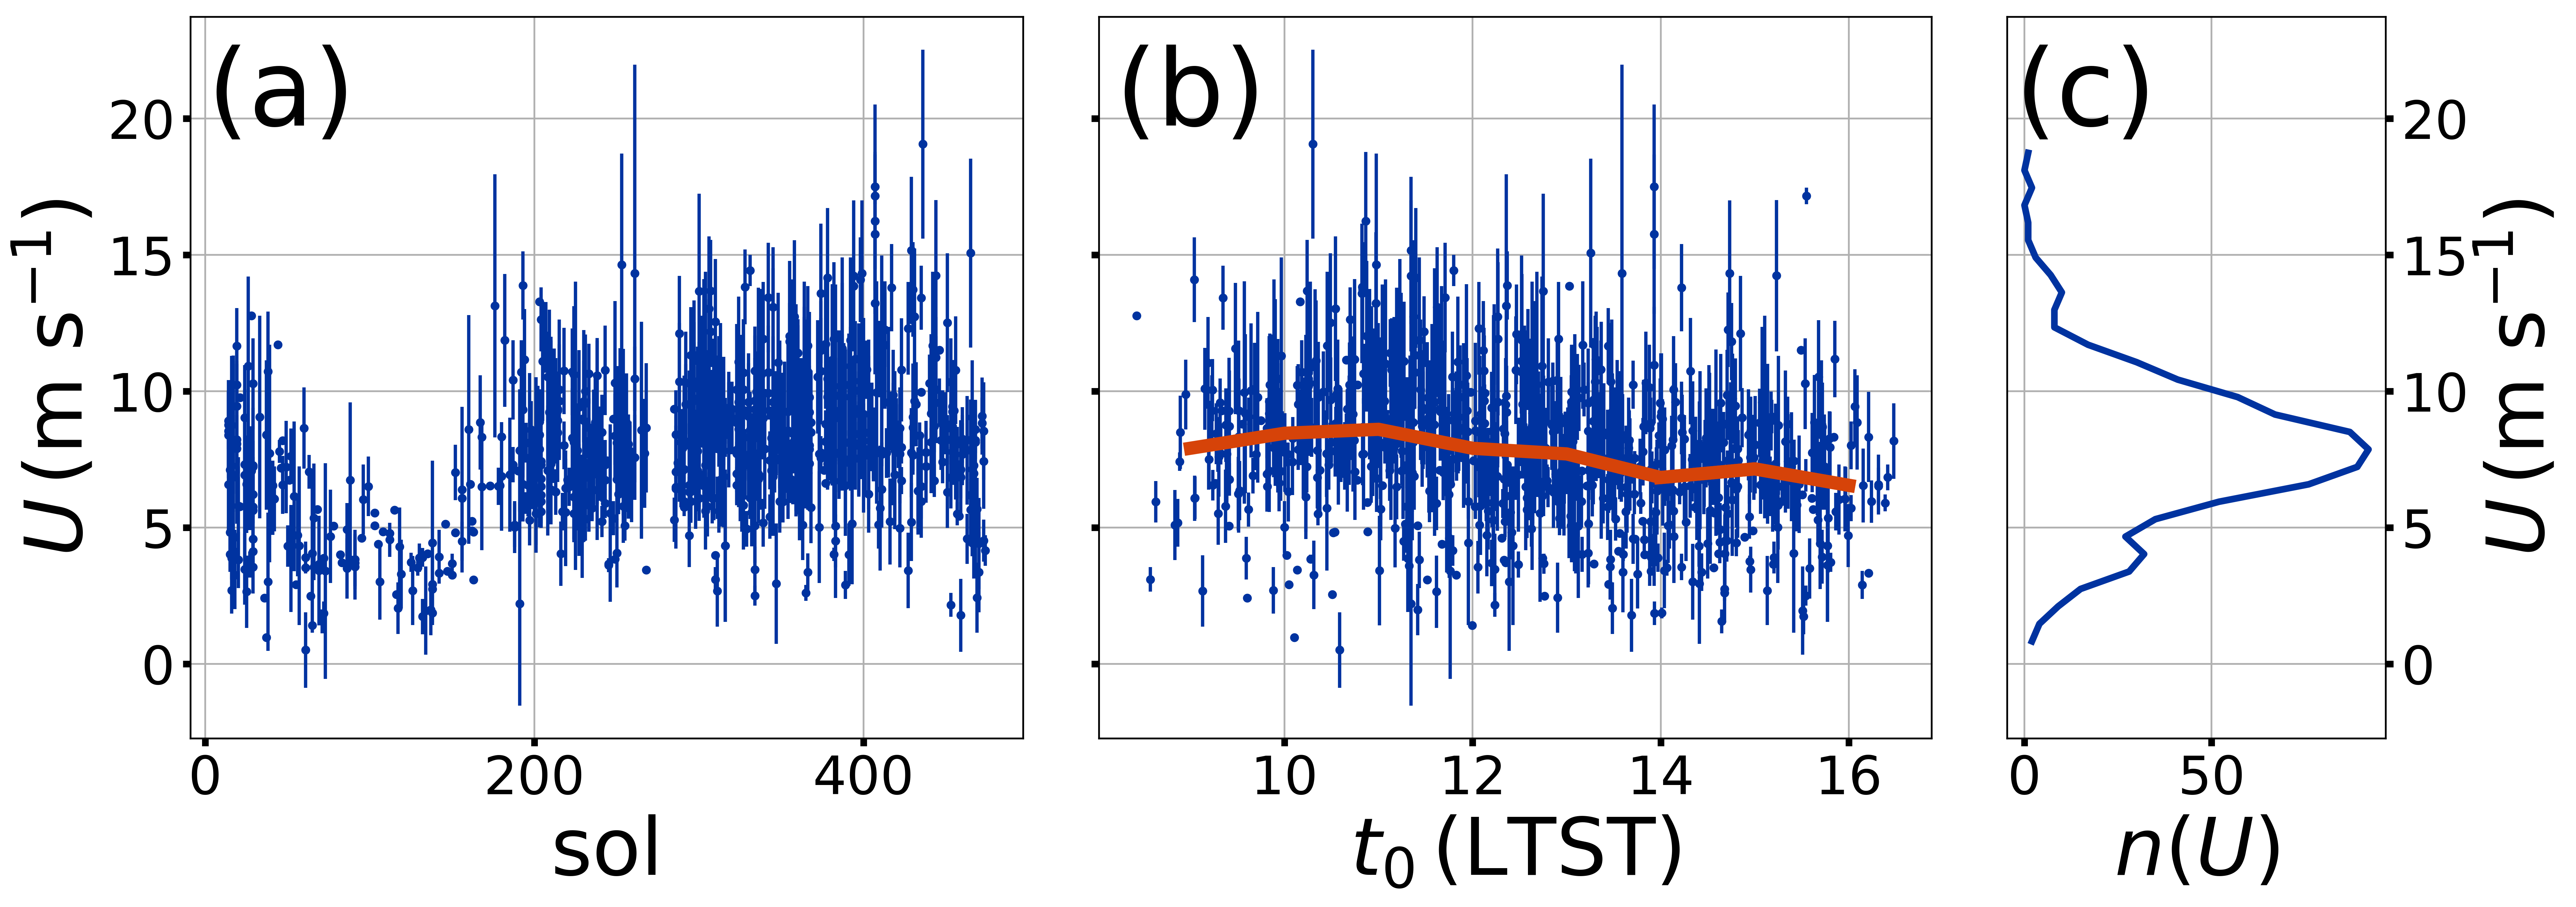
\includegraphics[width=\textwidth]{figures/U_vs_t0-sol_hist.png}
    \caption{Distribution of vortex-associated wind speeds $U$ as a function of time of day (a) and mission sol (b). Panel (c) shows a differential (as opposed to cumulative) histogram of $U$-values.}
    \label{fig:U_vs_t0-sol_hist}
\end{figure}

% \begin{figure}
%     \centering
%     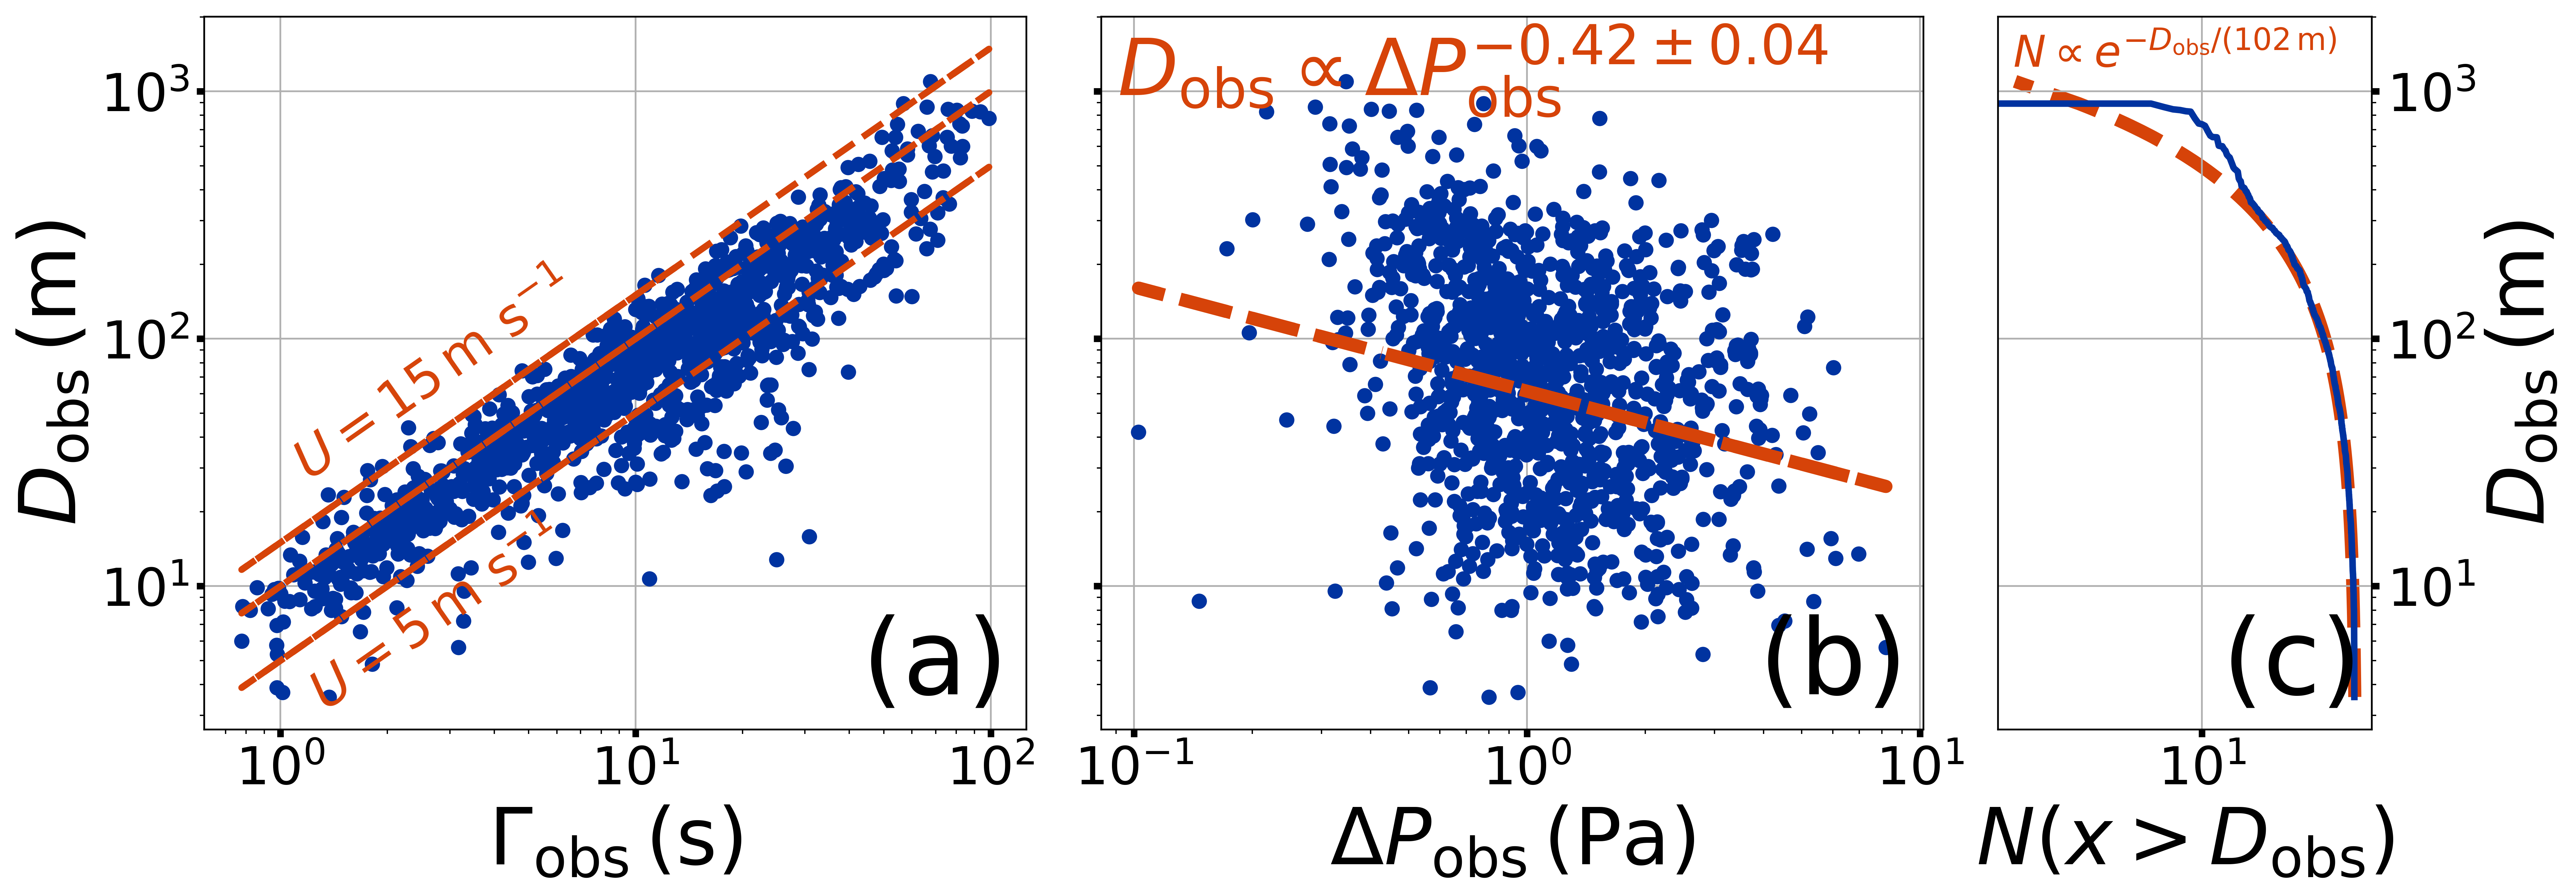
\includegraphics[width=\textwidth]{figures/Dobs_vs_Gammaobs-DeltaPobs_hist.png}
%     \caption{(a) Distribution of inferred vortex diameter $D_{\rm obs}$ from the observed $\Gamma_{\rm obs}$ (blue dots). Uncertainties on $D_{\rm obs}$ suppressed for clarity but are typically about $15\,{\rm m}$ or 10\% of $D_{\rm obs}$. Orange, dashed lines show a range of wind speeds $U$ -- $15$, $10$, and $5\,{\rm m\ s^{-1}}$ from top to bottom. (b) $D_{\rm obs}$ vs. each vortex's $\Delta P_{\rm obs}$. (c) Cumulative histogram of $D_{\rm obs}$, $N(x > D_{\rm obs})$ (blue curve), along with an exponential fit of the form $N \propto e^{D_{\rm obs}/D_0}$ with $D_0 = \left( 130.1 \pm 0.2 \right)\,{\rm m}$.}
%     \label{fig:Dobs_vs_Gammaobs-DeltaPobs_hist}
% \end{figure}

% 2021 Feb 4 - Double-checked the calib_event data. Wind speeds are recorded at 1 Hz instead of 0.5 Hz. Probably not going to make a big difference in my results.

Next, we couple our pressure profile and wind profile fits (Equations \ref{eqn:Lorentzian_profile} and \ref{eqn:wind_profile}) to infer the actual central pressure excursions $\Delta P_{\rm act}$ and vortex diameters $D_{\rm act}$, as well as the the eyewall wind velocities $V_{\rm act}$. The wind speed data showed considerable turbulent excursions not captured by our model, so as we fit the wind speed models, we inflated the data point and model parameter uncertainties by multiplying by the square root of the reduced $\chi^2$-values, effectively imposing $\chi^2 = 1$ \citep[cf.][]{Press2007}. We also propagated the uncertainties from the pressure and wind profile fit parameters into uncertainties on the actual parameters, as described in \ref{sec:Inferring Encounter Geometries from the Pressure and Velocity Profiles}. For these results, we only included encounters for which the inferred $b/D_{\rm act} \leq 1$, $V_{\rm obs}/\sigma \geq 3$, and with well-defined uncertainties on the actual values -- we found \boverDactltone\ such vortex encounters. 

The best-fit wind profile models are illustrated for the three representative vortex encounters in Figure \ref{fig:vortices_and_windspeed}, Figure \ref{fig:Dact_vs_Pact} shows the distribution of inferred $\Delta P_{\rm act}$- and $D_{\rm act}$-values. The minimum, median, and maximum values for $P_{\rm act}$ are $1.20\pm0.12$, $3.33\pm0.18$, and $16.6\pm4.5\,{\rm Pa}$, respectively, and for $D_{\rm act}$ are $7.70\pm2.19$, $59.1\pm17.6$, and $517\pm181\,{\rm m}$. Panels (b) and (c) show the cumulative histograms for $P_{\rm act}$ and $D_{\rm act}$, along with power-law fits. The fit for $P_{\rm act}$ appears to be significantly better than that for $D_{\rm act}$ and corresponds to a differential histogram with a power-law index $\gamma = -2.28$, significantly more shallow than the differential histogram for $P_{\rm obs}$ (with $\gamma = -3.39$). This result is qualitatively inconsistent with theoretical expectations that the distribution of actual pressure drops is steeper than (i.e., the magnitude of the power-law exponent is larger) or the same as the distribution of observed drops \citep{2014JAtS...71.4461L, 2018Icar..299..166J, 2019Icar..317..209K}.

\begin{figure}
    \centering
    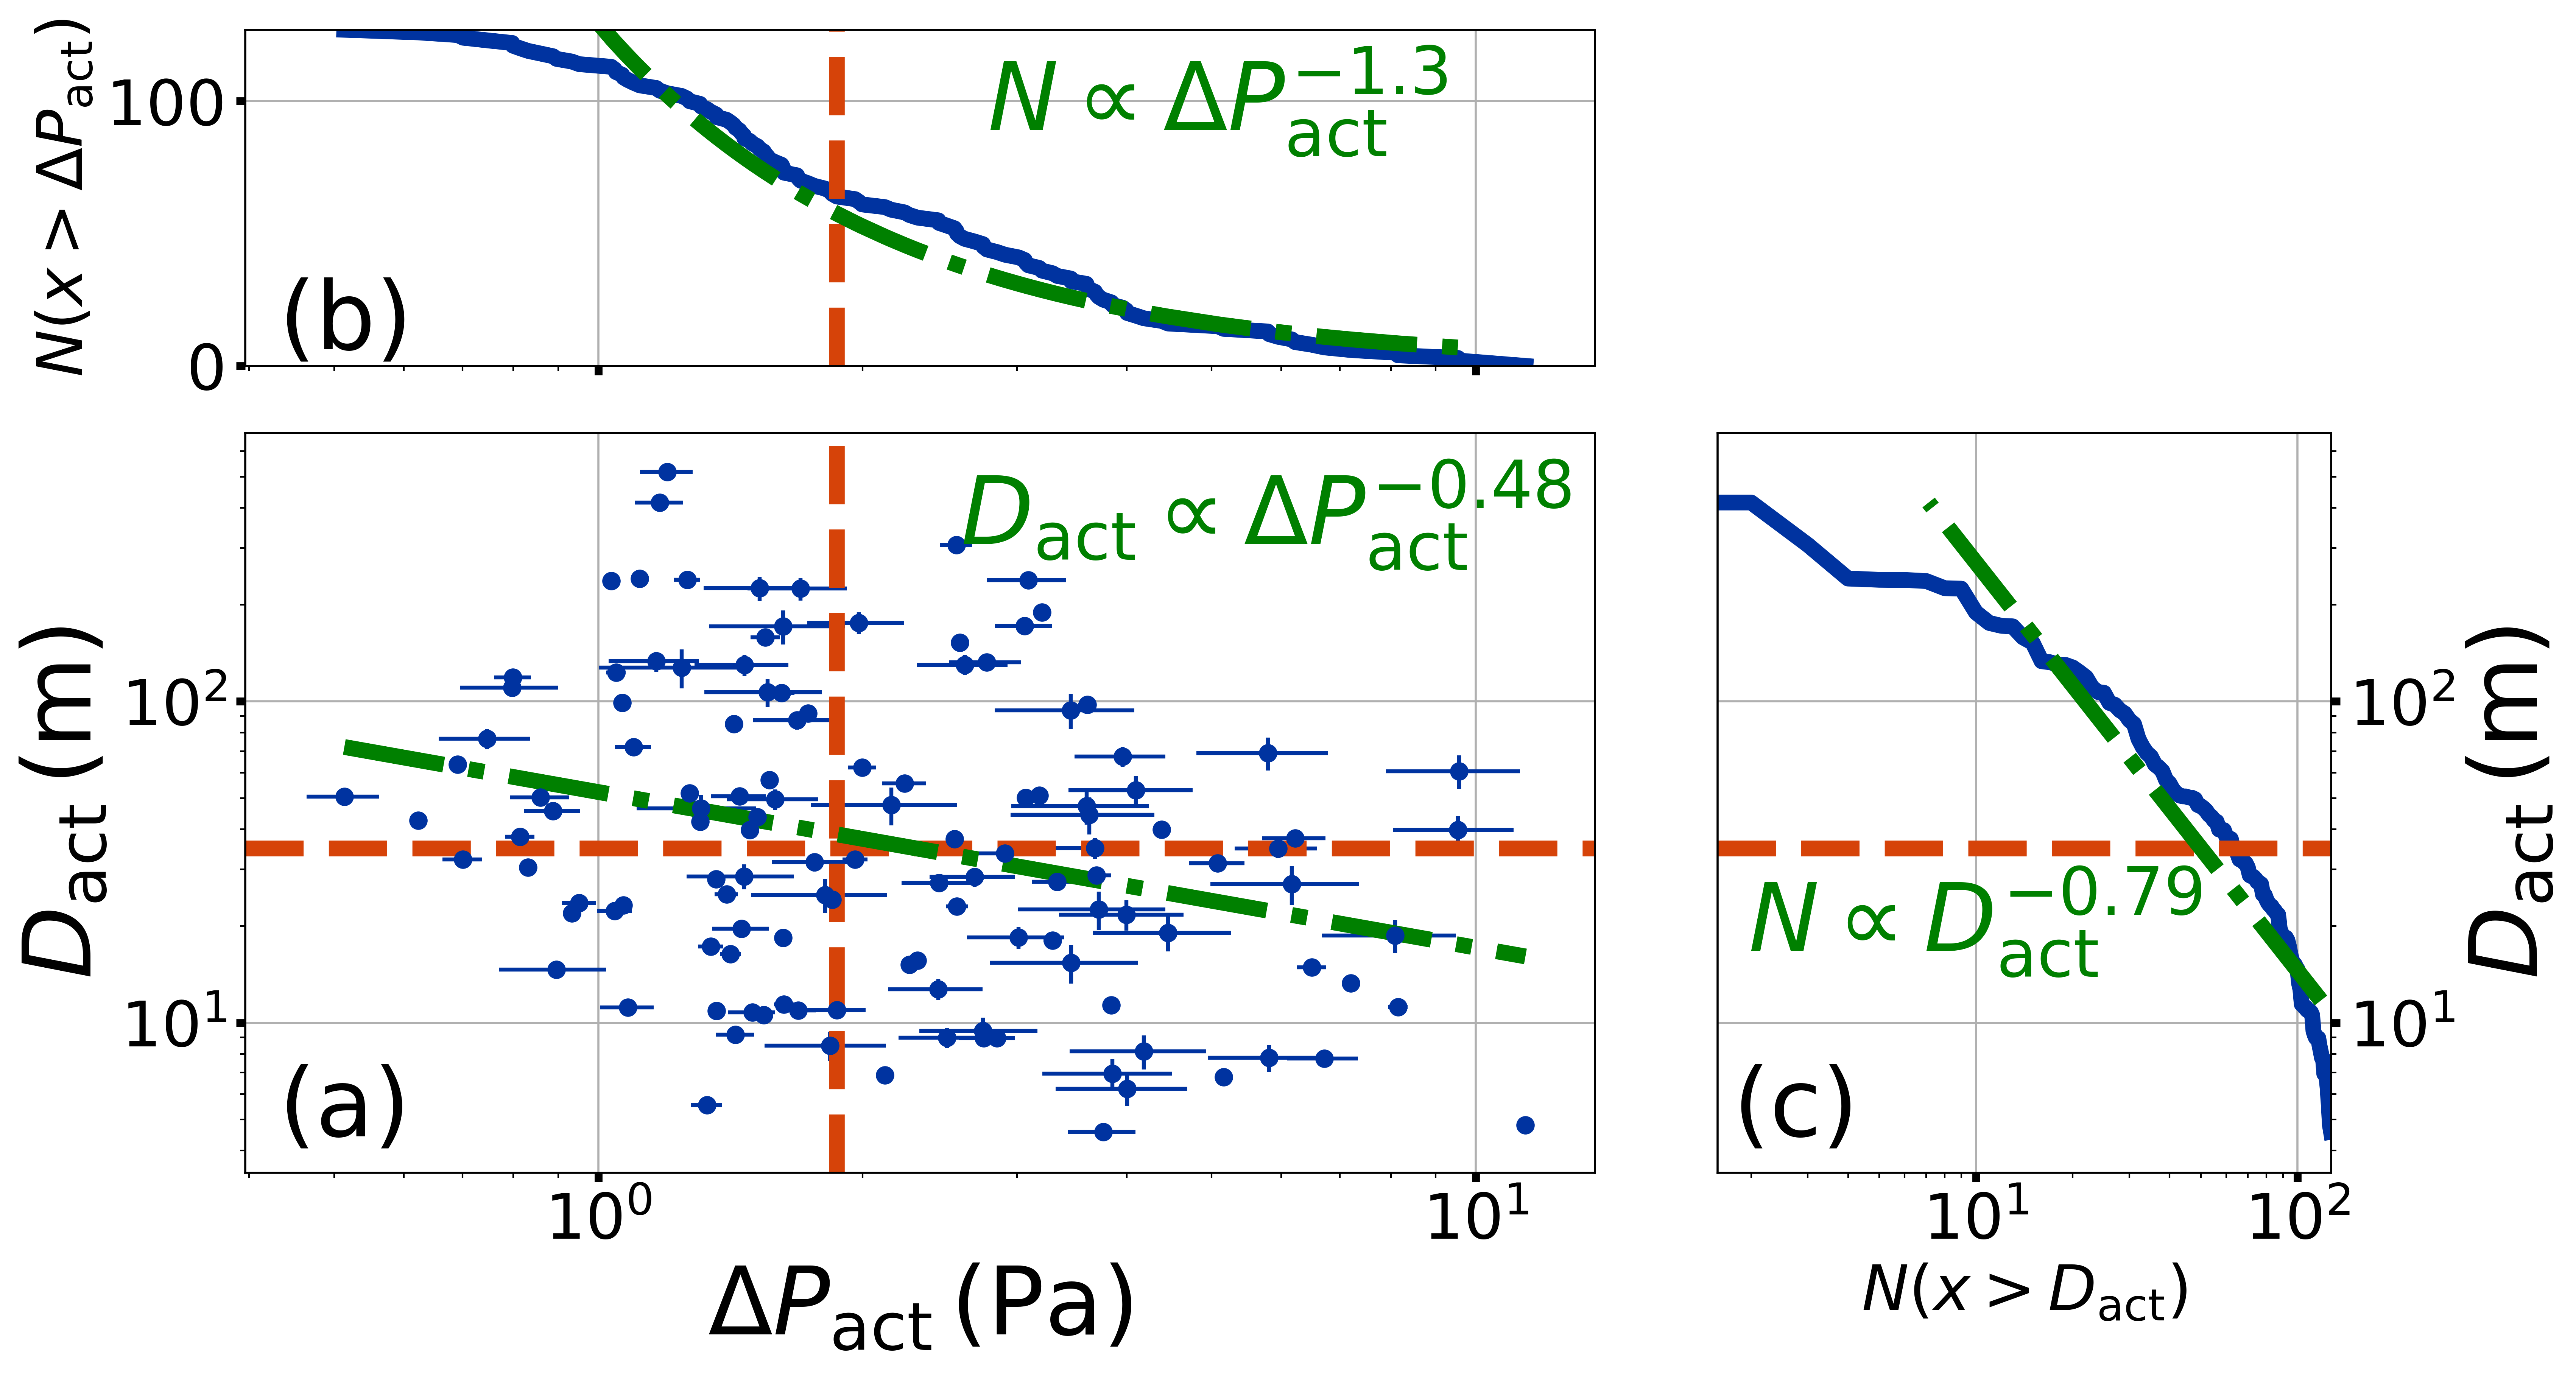
\includegraphics[width=\textwidth]{figures/Dact_vs_Pact.png}
    \caption{(a) Distribution of estimated actual vortex diameters $D_{\rm act}$ vs. the pressure excursions $\Delta P_{\rm act}$ (blue dots) with uncertainties, along with a power-law fit (dashed, orange line). (b) Cumulative histogram of $P_{\rm act}$-values. (c) Cumulative histogram of $D_{\rm act}$-values.}
    \label{fig:Dact_vs_Pact}
\end{figure}

This inconsistency likely arises from our choice to filter out distant encounters ($b/D_{\rm act} > 1$) and low-signal vortices ($V_{\rm obs}/\sigma < 5$). All else being equal, vortices with small $\Delta P_{\rm act}$ are also likely to have small $V_{\rm act}$ and therefore to register with small $V_{\rm obs}$ in an encounter. \citet{2020Icar..33813523J} also suggested that $D_{\rm act} \propto \Delta P_{\rm act}^{1/2}$, meaning small $\Delta P_{\rm act}$ are more likely to have $b/D_{\rm act} > 1$. Indeed, a power-law fit to the distribution of $D_{\rm act}$ vs.~$\Delta P_{\rm act}$ gives $D_{\rm act} \propto \Delta P_{\rm act}^{-0.34}$, although the distribution is also statistically consistent with no correlation as well. 

\begin{figure}
    \centering
    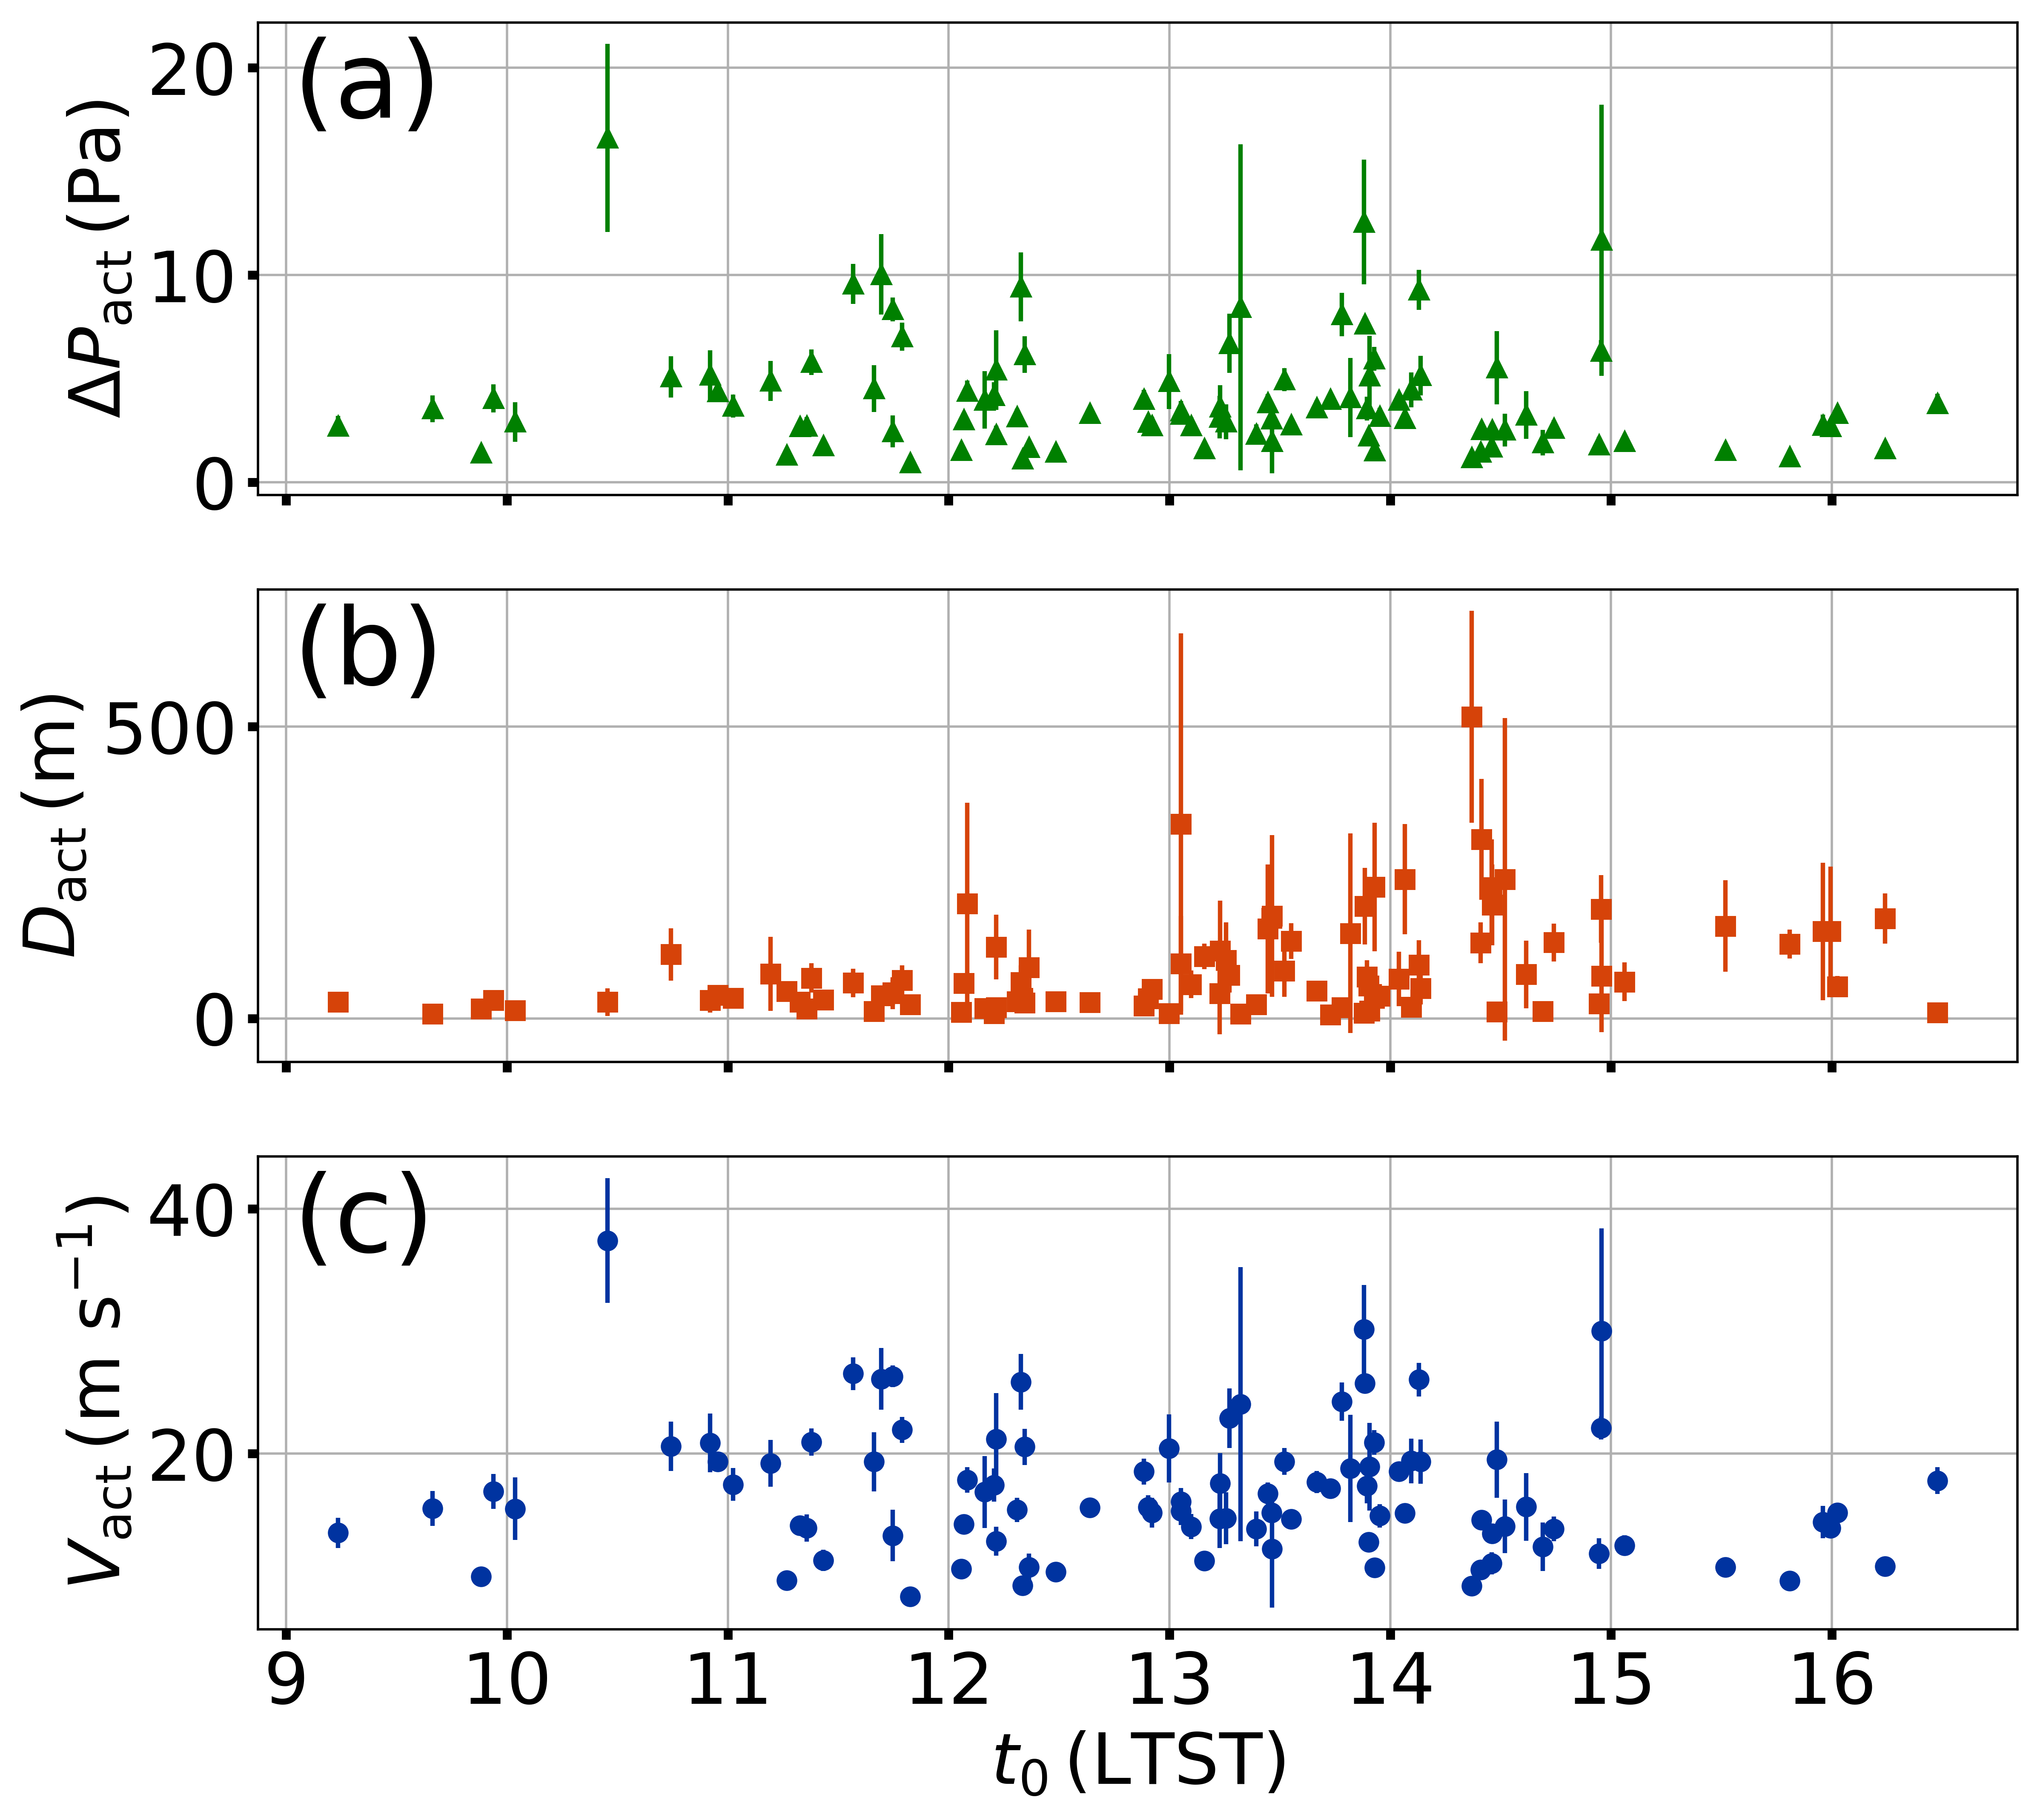
\includegraphics[width=0.5\textwidth]{figures/all_actual_values_vs_t0.png}
    \caption{(a) Distributions of $\Delta P_{\rm act}$ (a), $D_{\rm act}$ (b), and $V_{\rm act}$ (c) with time-of-day $t_0$ (local true solar time, LTST). The dashed, grey horizontal line in panel (c) is a putative threshold below which a vortex might not lift dust.}
    \label{fig:all_actual_values_vs_t0}
\end{figure}

In spite of these observational biases, we can still infer eyewall velocities $V_{\rm act}$ and look at trends with time-of-day $t_0$. Figure \ref{fig:all_actual_values_vs_t0} shows how $\Delta P_{\rm act}$, $D_{\rm act}$, and $V_{\rm act}$ as functions of time-of-day $t_0$. The min, median, and maximum values for $V_{\rm act}$ are $9.17\pm0.48$, $15.6\pm1.0$, and $37.4\pm5.1\,{\rm m\ s^{-1}}$. The trends for all parameters with $t_0$ seem reasonable: many of the largest values for all parameters occur in the late afternoon, although the very largest values for each do not always occur late in the day. 

\begin{figure}
    \centering
    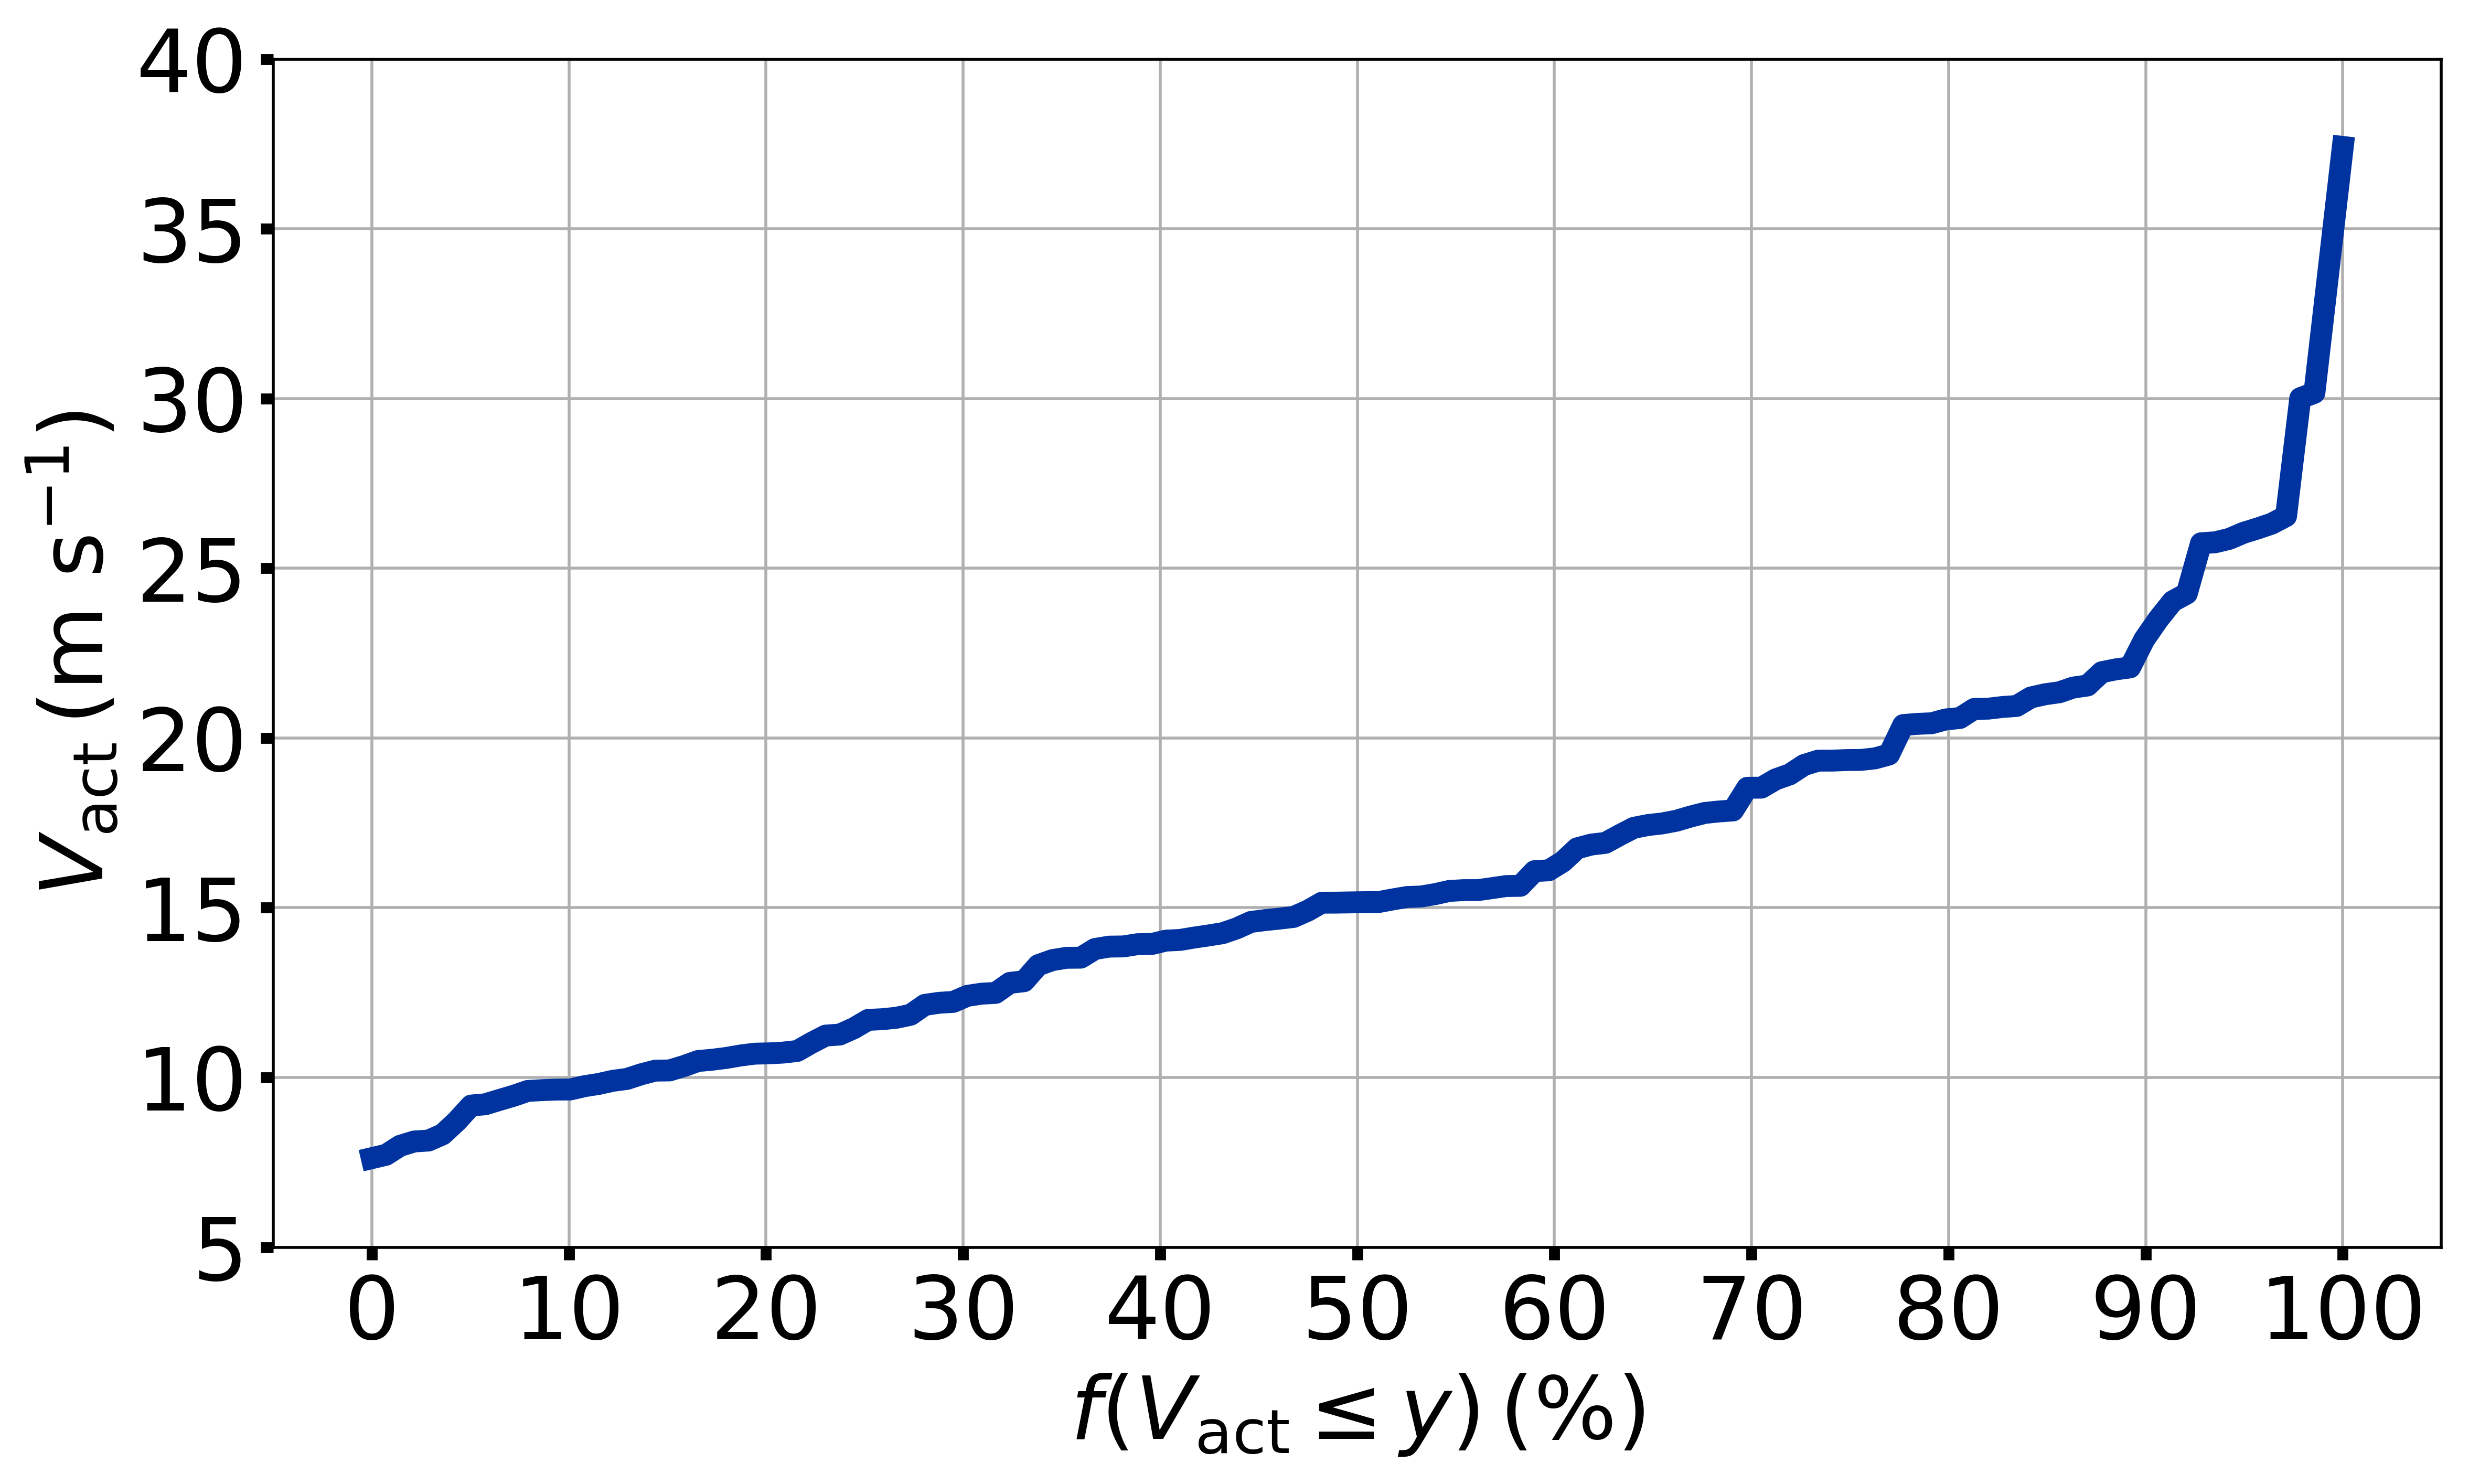
\includegraphics[width=0.5\textwidth]{figures/cum_hist_Vact.png}
    \caption{The fractional cumulative histogram of inferred $V_{\rm act}$-values. For example, about 20\% of the vortices we analyzed have $V_{\rm act} \geq 20\,{\rm m\ s^{-1}}$.}
    \label{fig:cum_hist_Vact}
\end{figure}

% 30 m/s threshold
% \citep{2003JGRE..108.5041G, 2006JGRE..11112002C, 2011GeoRL..3824206C}

\subsection{Inferring Areal Occurrence Rate from the Time-Series Analysis}
\label{sec:Inferring Dust Devil Density from the Time-Series Analysis}

\begin{figure}
    \centering
    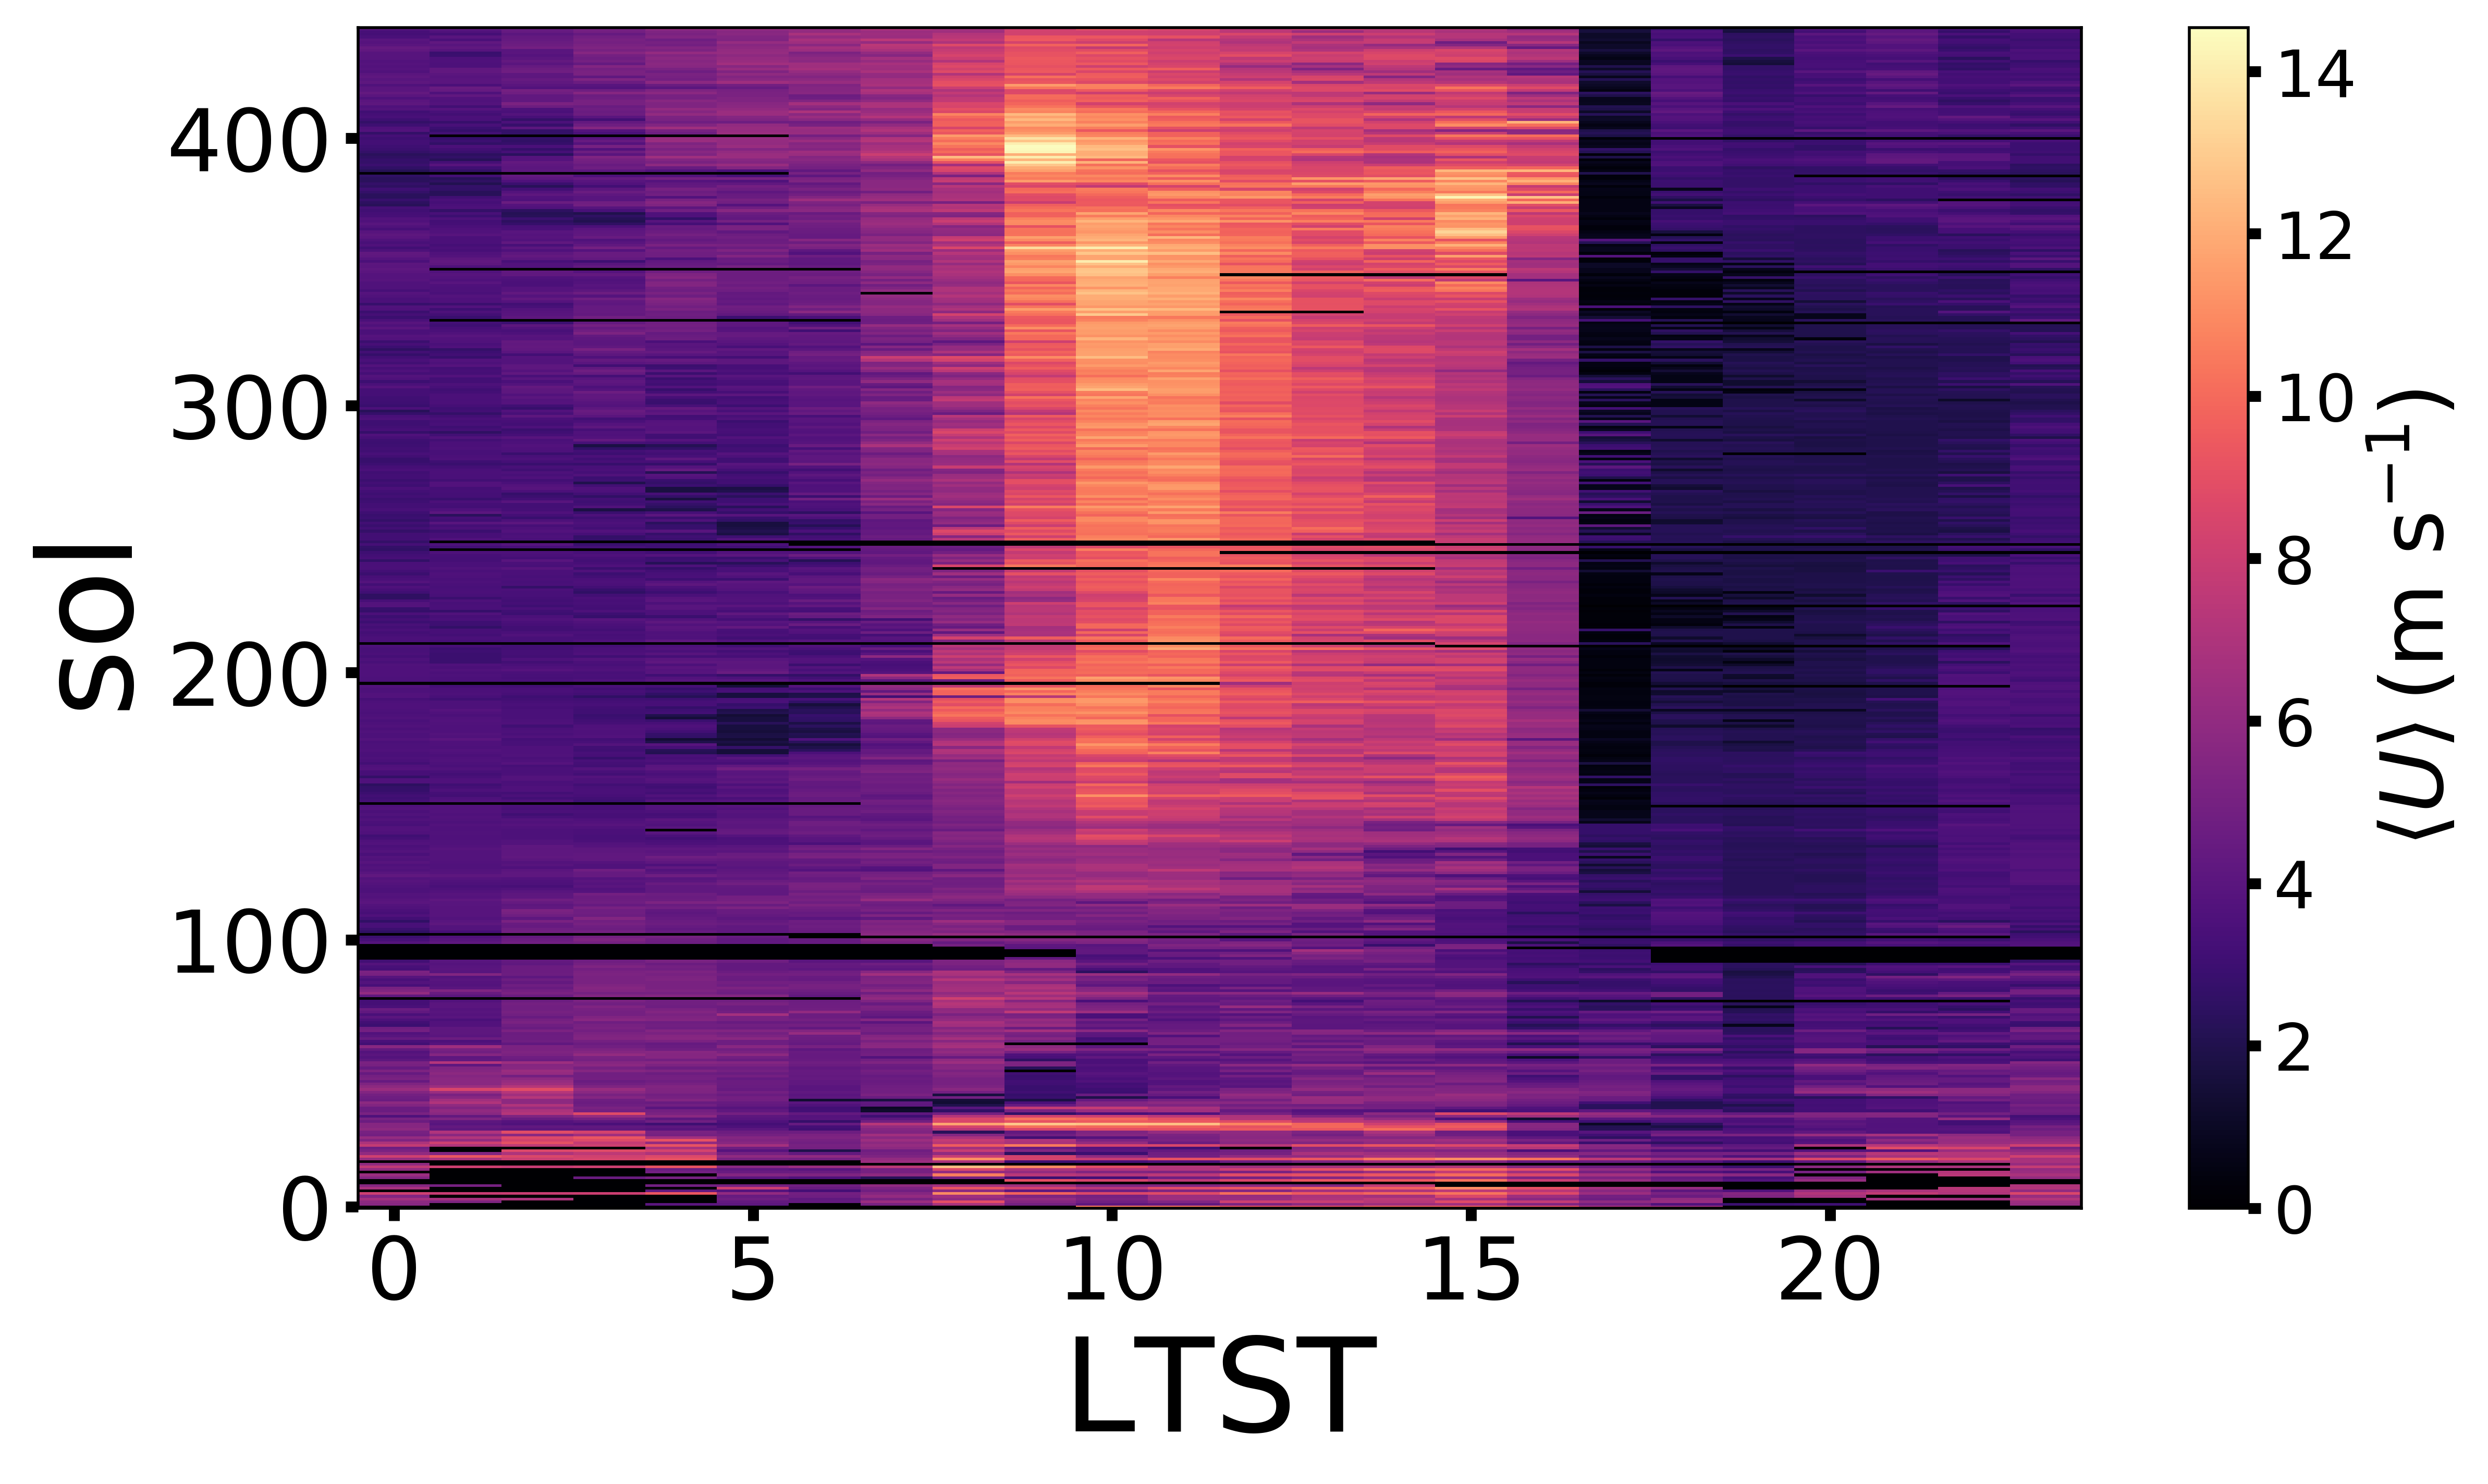
\includegraphics[width=\textwidth]{figures/advective_speeds.png}
    \caption{The hour-by-hour average wind speeds $\langle U \rangle$ for each sol. Brighter (yellower) colors represent higher speeds.}
    \label{fig:advective_speeds}
\end{figure}

If all encountered vortices had the same advective speed $U$, diameter $D_{\rm act}$, and central pressure excursion $\Delta P_{r\m act}$, the areal density of vortices $n$ can be estimated from the number of vortex detections per unit time, $\nu$, via
\begin{equation}
    \nu = k/T = n U \left( 2 b_{\rm max} \right) \label{eqn:simple_number_of_encounters}
\end{equation}

where $k$ is the total number of encounters during the observing period $T$ and $b_{\rm max} = \left( \frac{D_{\rm act}}{2} \right) \sqrt{ \frac{\Delta P_{\rm act}}{\Delta P_{\rm min}} - 1 }$ is the maximum radial encounter distance for which a pressure signal will register. For the advective speed, we use not the pre-encounter wind velocities considered in, for example, Equation \ref{eqn:total_wind_speed} but the hour-by-hour or sol-by-sol average speeds illustrated in Figure \ref{fig:advective_speeds} because we are interested in the advection of a population of vortices, not the individual vortices. In principle, calculating $N$ from the observed encounters requires integrating over the population. Unfortunately, the small number of vortices for which we were able to robustly estimate the actual parameters severely limits our ability to integrate over the population.  Moreover, we expect these parameters to vary with time-of-day and season. In lieu of this more complete evaluation, we instead calculate the population average for $b_{\rm max}$ and then use that average value to solve for $n$ from the encounter rates depicted in Figure \ref{fig:sol_and_t0_histograms}. Figure \ref{fig:areal_occurrence_rate} shows our estimate for the areal occurrence rate for vortices.

\begin{figure}
    \centering
    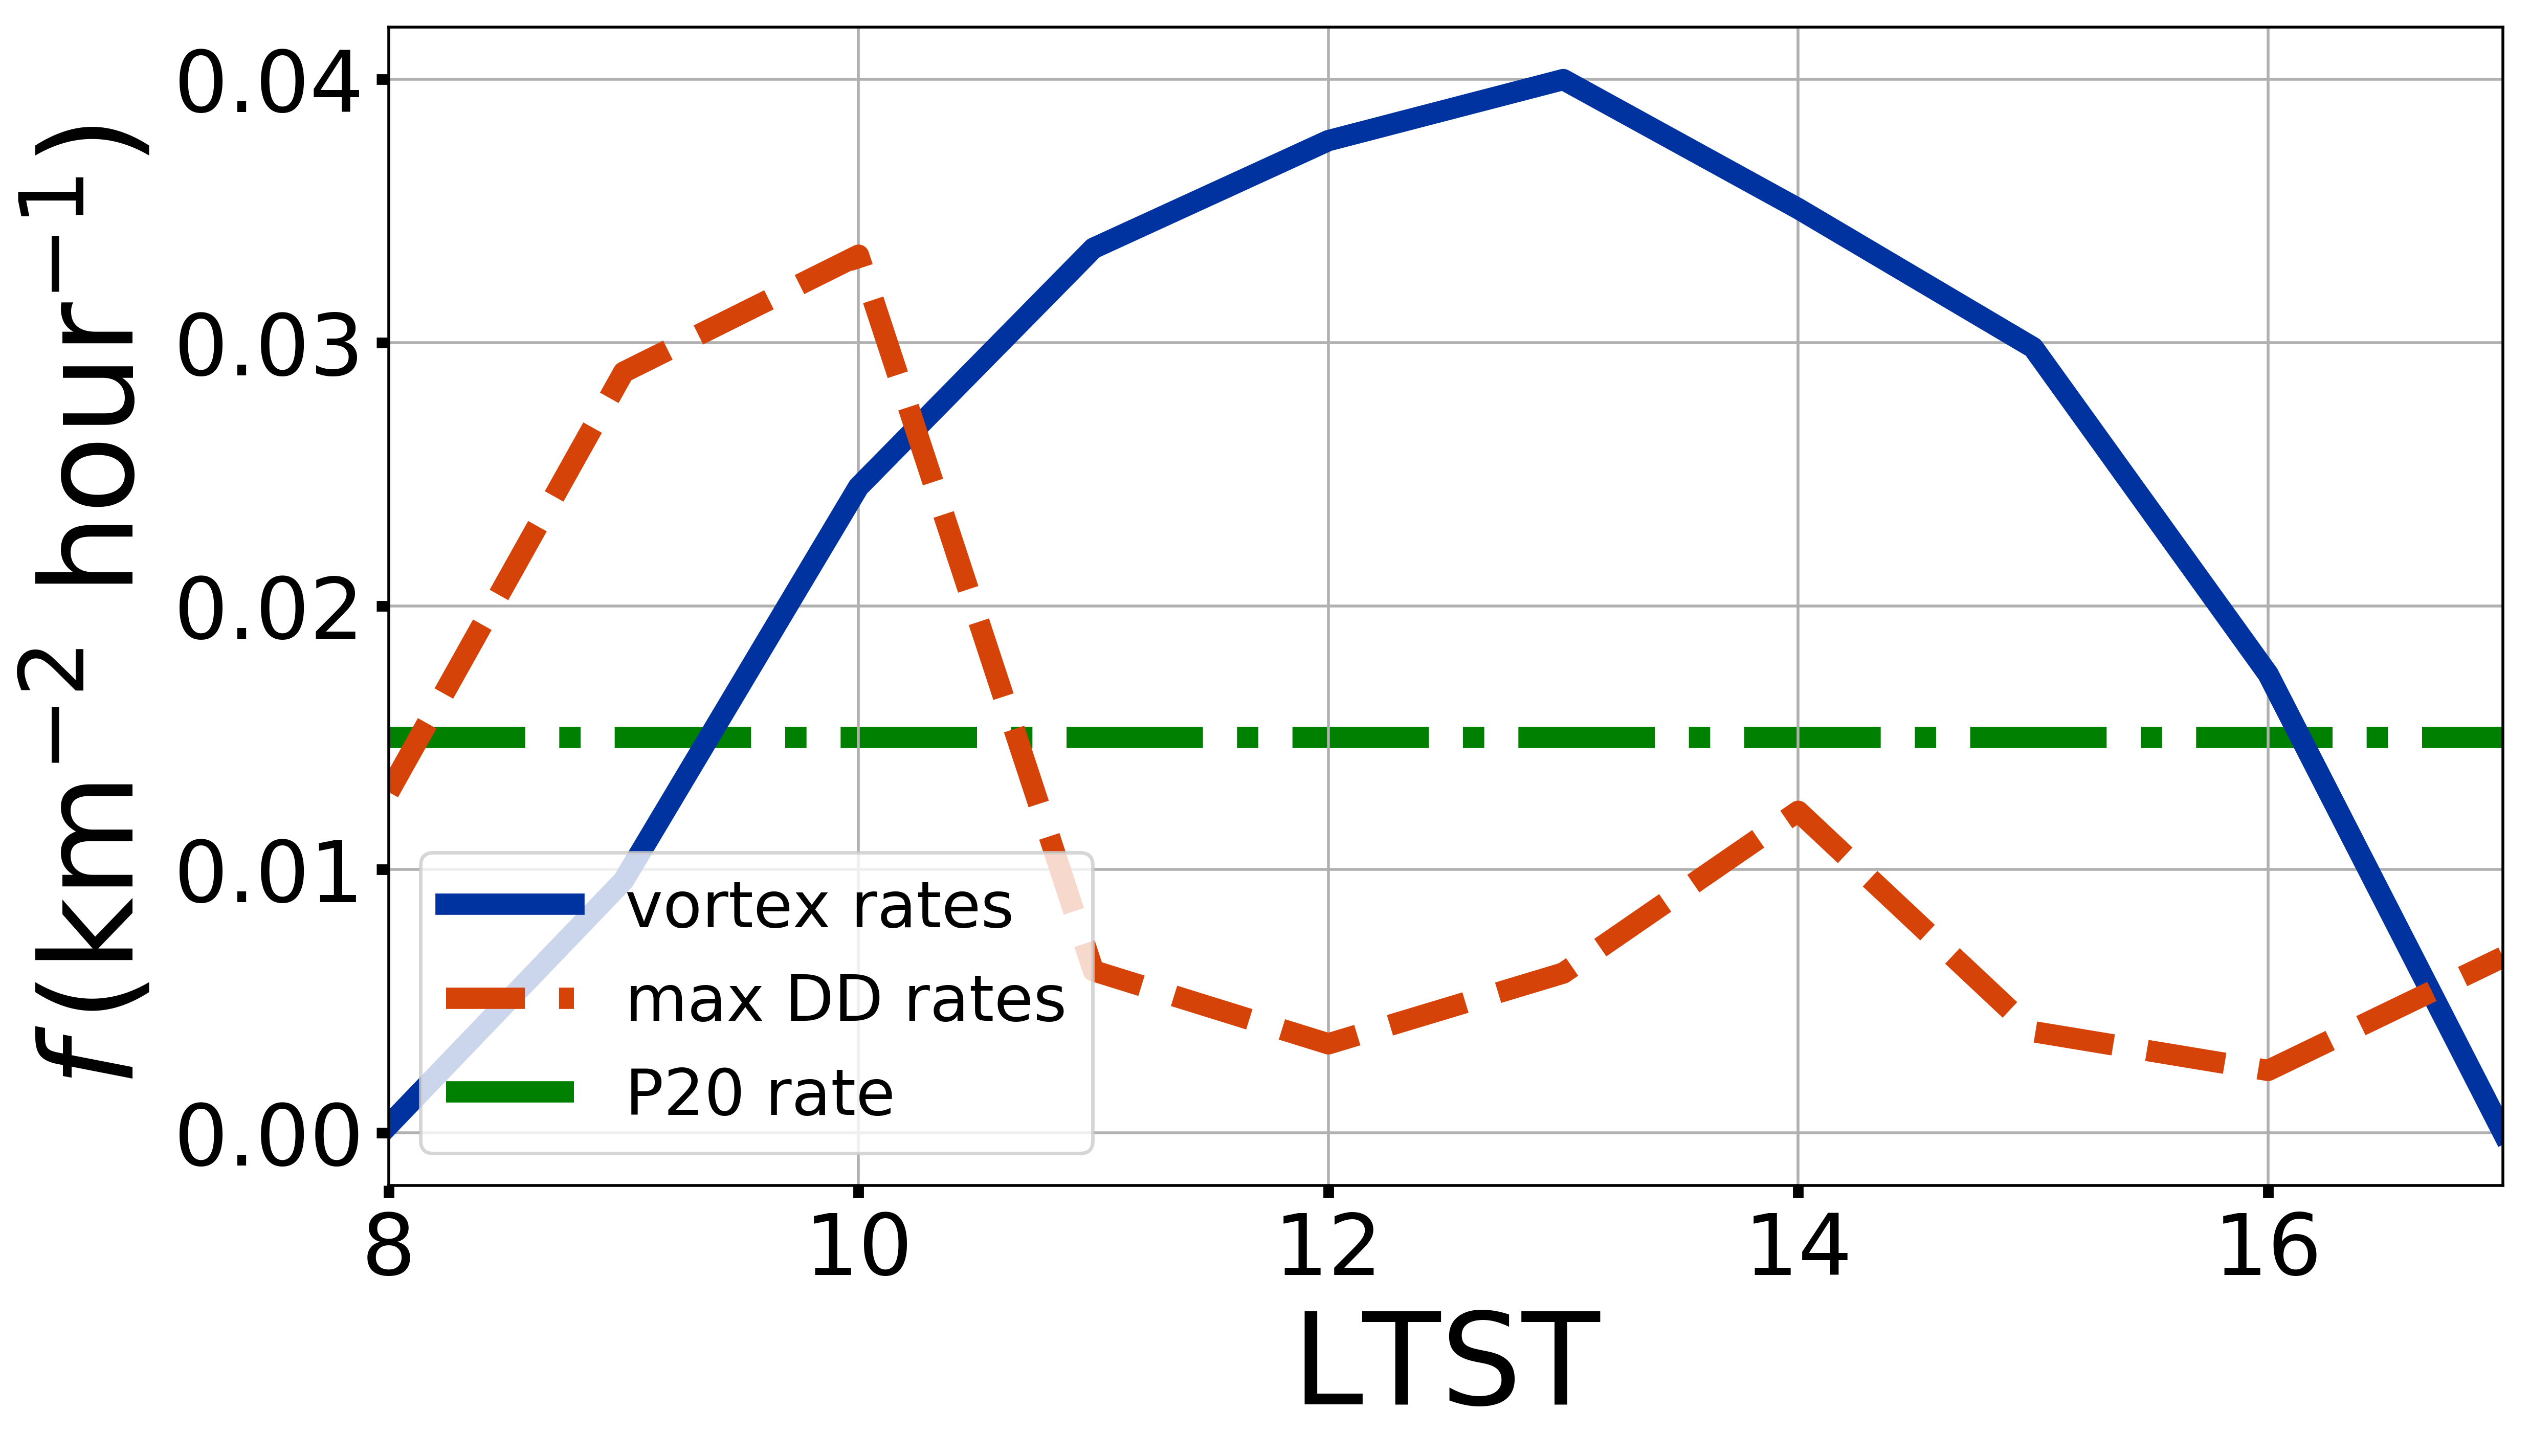
\includegraphics[width=\textwidth]{figures/areal_occurrence_rate.png}
    \caption{The solid blue curve shows the areal occurrence rate for vortices (``vortex rates''). The dashed, orange line shows the allowed maximum rate for dust devils inferred from the image analysis (``max DD rates''). The grey region shows a range of rates reported in \citet{2020GeoRL..4787234P} (``P20 rate'').}
    \label{fig:areal_occurrence_rate}
\end{figure}

% Figure \ref{fig:areal_density} show the resulting areal density estimates. We find the estimated areal densities largely follow increases and decreases in the encounter rate. The peak in the hour-by-hour density at 13:00 LTST is slightly more pronounced than the peak in the corresponding encounter rate because of a slightly higher average advective speed around 12:00 LTST. 

% \begin{figure}
%     \centering
%     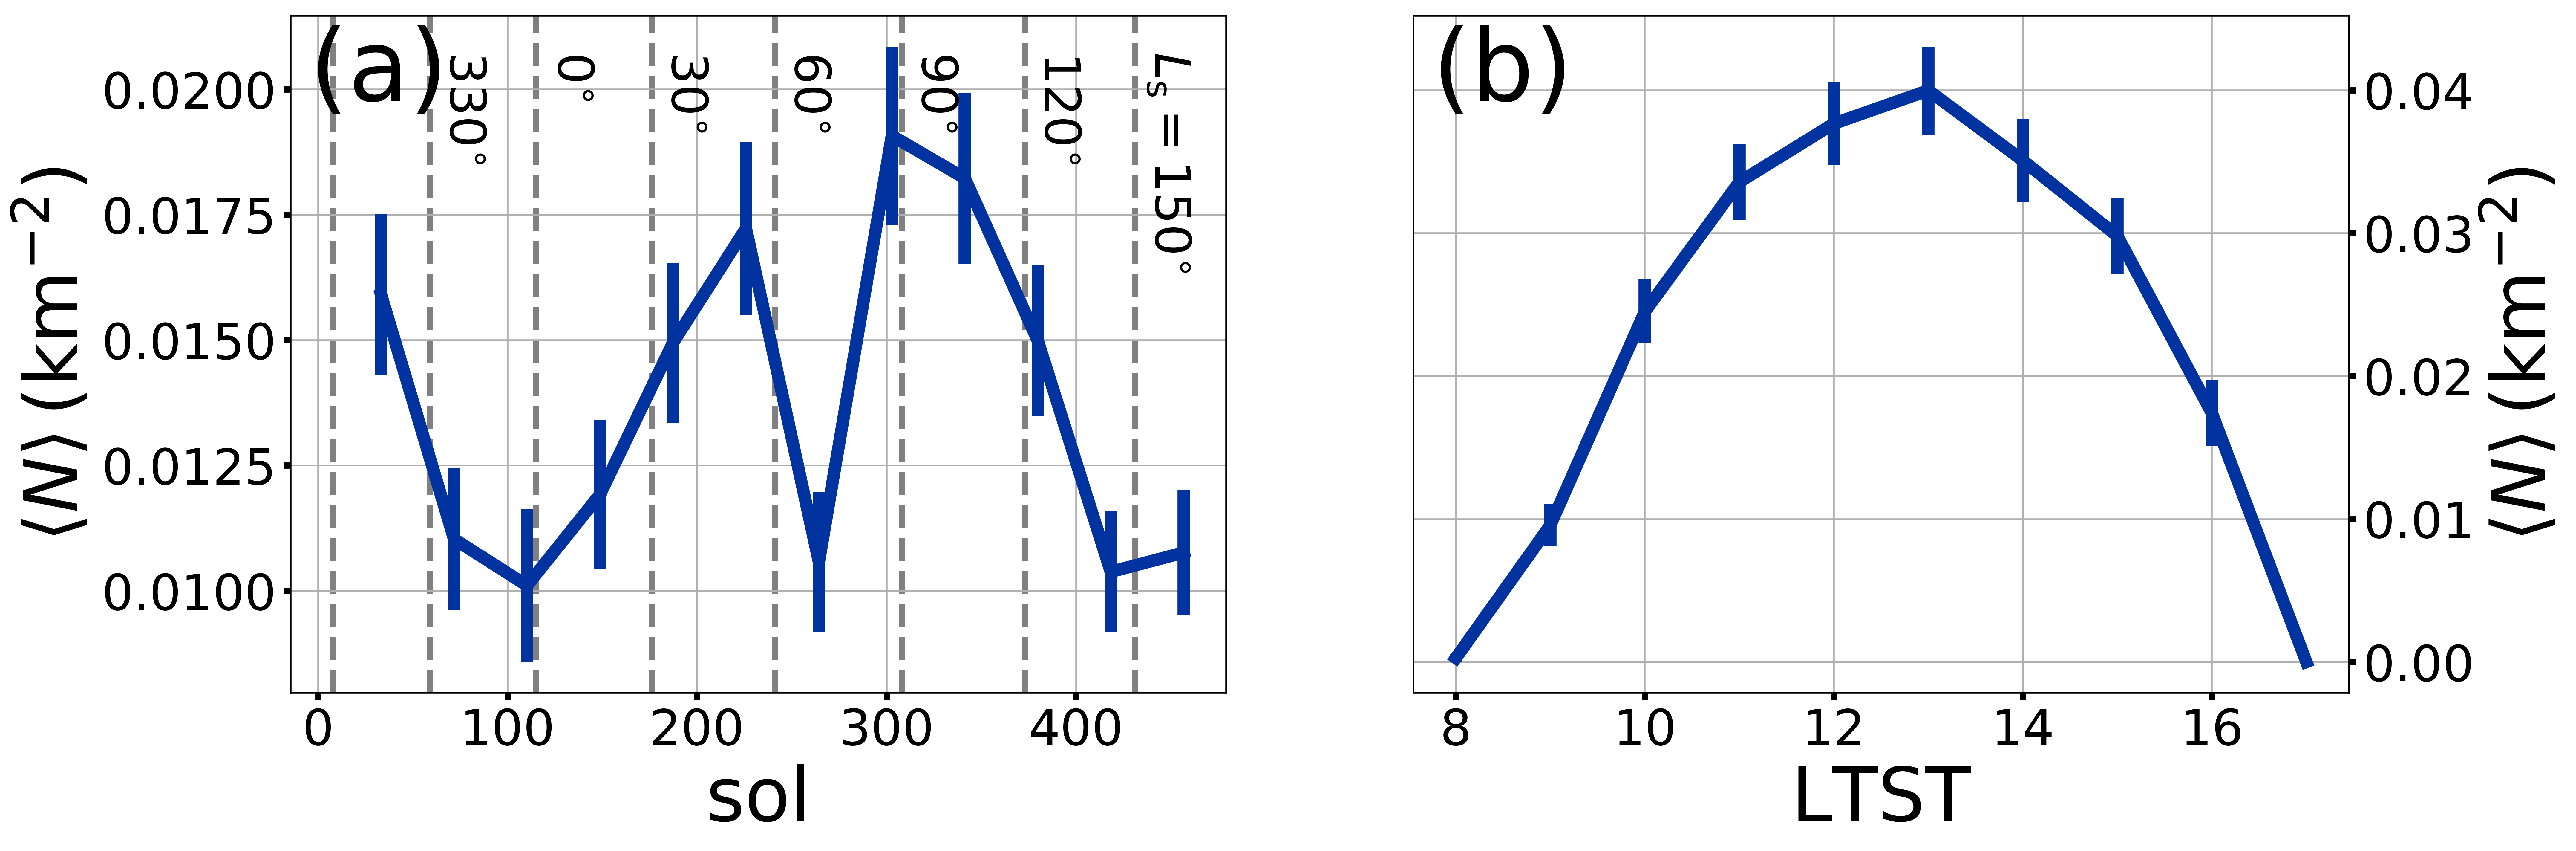
\includegraphics[width=\textwidth]{figures/areal_density.png}
%     \caption{(a) Areal density by sol binned as in panel (a) of Figure \ref{fig:sol_and_t0_histograms}. (b) Areal density by hour with the same binning as in panel (b) of Figure \ref{fig:sol_and_t0_histograms}.}
%     \label{fig:areal_density}
% \end{figure}

\section{Image Analysis}
\label{sec:Image Analysis}

\begin{figure}
    \centering
    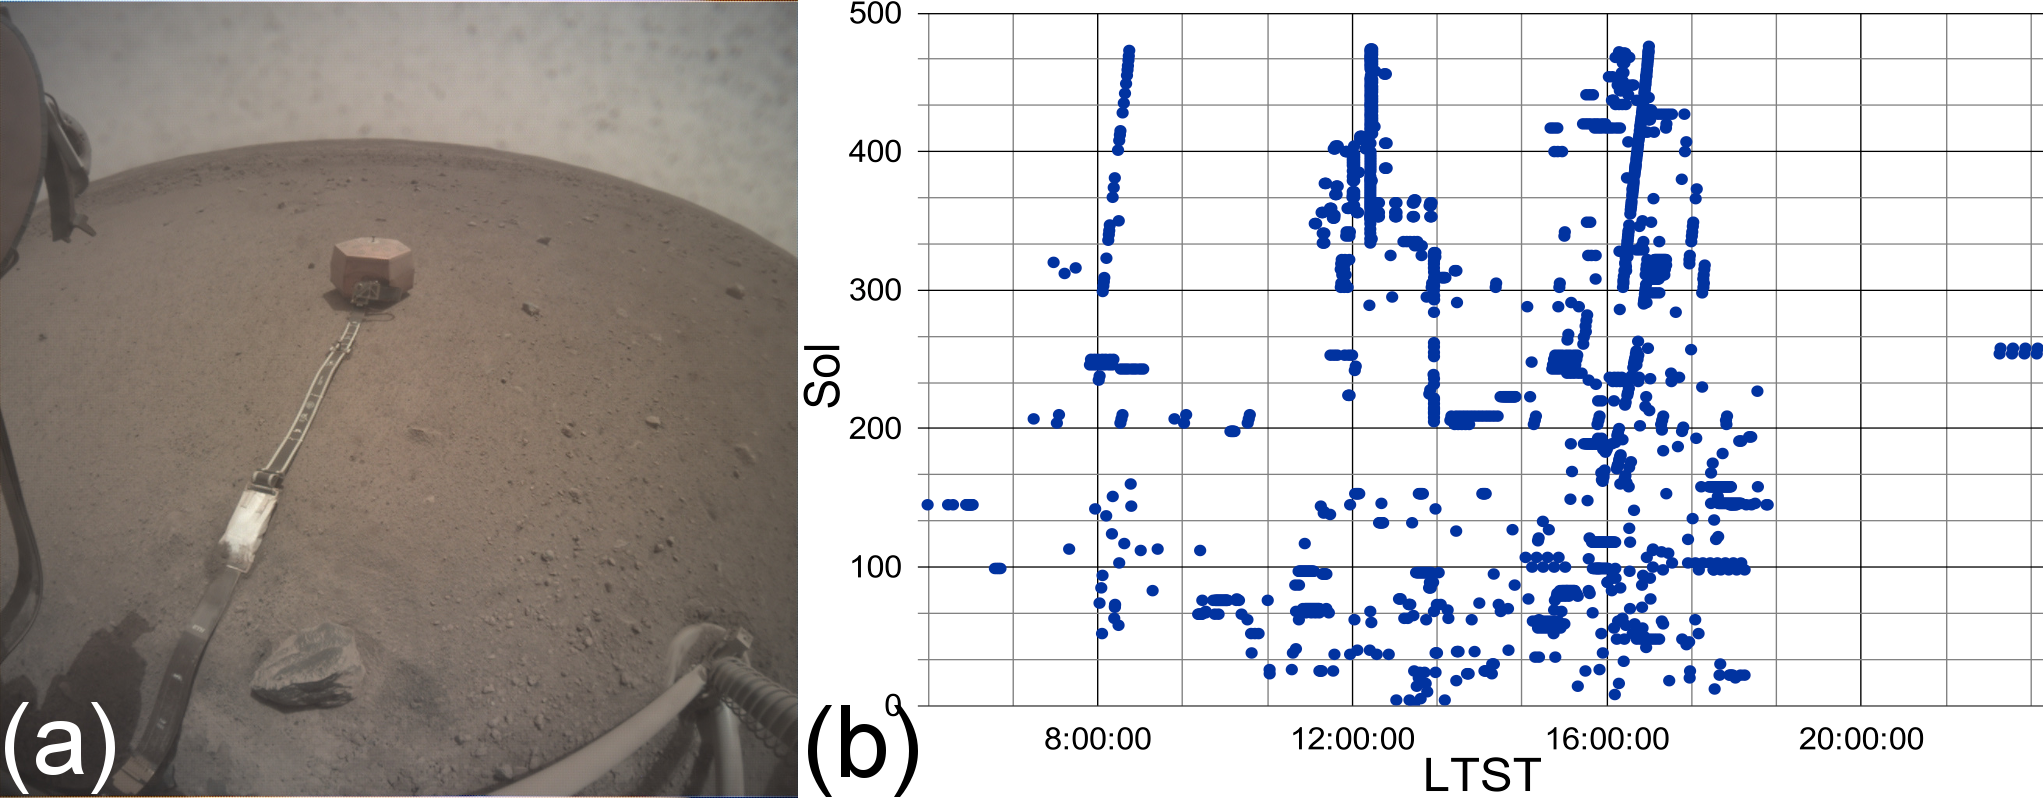
\includegraphics[width=\textwidth]{figures/Example-Image_Insight-Combined-Analysis.png}
    \caption{(a) Example of an Instrument Context Camera (ICC) image. (b) Times and sols during which images were collected throughout the InSight mission.}
    \label{fig:Example-Image_Insight-Combined-Analysis}
\end{figure}

In this section, we describe our analysis of image data from InSight to search for the passage of dust devils. To cut to the chase, our survey detected no active dust devils, but we can provide an upper limit on their activity based on the geometry, frequency, and timing of observations.

% How many images and TOD of observations

For our visual dust devil survey, we use observations from InSight's Instrument Context Camera (ICC) because that camera is mostly consistently pointed toward the horizon. ICC has a field-of-view (FOV) of $124^\circ\times124^\circ$ and sits about $0.7\,{\rm m}$ off the surface \citep{2018SSRv..214..105M} -- Figure \ref{fig:Example-Image_Insight-Combined-Analysis}(a) shows an example image. As of this manuscript's preparation, the NASA PDS archive for ICC contains images spanning sols 1 to 476 (although many sols lack images), totaling \numICCimages\ images. Figure \ref{fig:Example-Image_Insight-Combined-Analysis}(b) shows the sols and times when images are available. Even though none of the images show active dust devils, we can still translate them into an upper limit on dust devil activity by considering the area and times surveilled. 

% Brief description of camera including FOV and distance to horizon and surveyed area
The local topography limits the horizon for the Instrument Deployment Camera (IDC) toward the south to about $2.4\,{\rm km}$ \citep{2020E&SS....701248G}. Since ICC is even closer to the ground ($0.7\,{\rm m}$ vs.~IDC's $1.5\,{\rm m}$), the view is even more limited. However, as an upper limit, we can estimate the area surveilled as $\frac{1}{2} \pi \left(124^\circ/180^\circ\right) \left( 2.4\,{\rm km} \right)^2 \approx 6.2\,{\rm km^2}$. An important limitation of this approach: smaller dust devils cannot be resolved at the same maximum distance as larger devils. However, ICC has an angular resolution of $\alpha = 2\times10^{-3}\,{\rm rad\ px^{-1}}$ \citep{2018SSRv..214..105M}, meaning we could resolve the diameter of the smallest vortex we detected ($D_{\rm act} = 7.7\,{\rm m}$) to a distance of about $3.9\,{\rm km}$, farther than the horizon.

% Wind speeds during observations
The chances of spotting a dust devil also depend on the time for it to cross through the area surveilled (assuming the lifetime of the dust devil is long by comparison). The maximum crossing time would give us the greatest chance to spot a dust devil and therefore the largest allowed areal occurrence rate consistent with no detections. This maximum time is equal to the time for a dust devil to cross along the horizon, no farther away than $2.4\,{\rm km}$. With an FOV of $124^\circ$, this distance is $\pi \left(124^\circ/180^\circ\right) \left( 2.4\,{\rm km} \right) \approx 2.6\,{\rm km}$. The time to cross this distance will depend on the ambient wind speed, and so for our calculation, we will take the median wind speed during each observational period. The resulting upper limits on the areal occurrence rate are shown in Figure \ref{fig:areal_occurrence_rate}. (Given that most sols have only one or a few images available, the areal occurrence rate binned by sol is much less informative, and so we do not include it.) 

\section{Discussion}
\label{sec:Discussion}

Altogether, these results invite several interesting conclusions which are bolstered by and contrasted with previous studies. The lack of observed dust devils in the ICC imagery indicates that the martian vortices are frequently dustless and therefore invisible (at least to the limit of the image contrast). Dustless vortices are certainly common on Earth, and there is no requirement that a vortex lofts dust, even when dust is available. In a terrestrial field experiment, \citet{LORENZ20151} found about 40\% of encountered vortices exhibited signatures consistent with dust loading. \citet{2016Icar..278..180S} reported 245 vortices encountered by the Mars Science Laboratory and found only two with clear signatures of dust-loading. Figure \ref{fig:areal_occurrence_rate} shows the maximum areal occurrence rates for dust devils allowed by the image survey, and comparing to the rates of vortex occurrence suggests no more than 35\% of the encountered vortices could have lofted dust and still not have registered in the images, roughly consistent with the terrestrial results. 

% Indeed, \citet{2020GeoRL..4787234P} conducted survey of images from InSight's ICC and found no signs of dust-bearing vortices, even though they reported more than 6000 vortex encounters. Given the observations of active trail formation observed in the vicinity of InSight \citep{2016Icar..266..315R, 2020GeoRL..4787234P}, this result seems surprising. As we discuss in the next section, however, the infrequent observations and small viewing area of ICC images conspire to reduce the significance of the non-detection of dust devils. In any case, we can combine the lack of observed dusty vortices with our time-series analysis to constrain, for example, the threshold wind velocities required for dust lifting on Mars. First, however, we need to calculate the underlying areal density of vortices from the encounter statistics in Figure \ref{fig:sol_and_t0_histograms}. 

% Inferring threshold wind speeds -- check that you didn't already!

% XXX INCLUDE caveat about dust devil size being a limiting factor for detection!
In fact, based on our non-detection of active dust devils and distribution of $V_{\rm act}$-values, we can estimate a minimum wind speed required to loft dust. If only 35\% of vortices lofted dust, Figure \ref{fig:cum_hist_Vact} suggests a threshold of $19\,{\rm m\ s^{-1}}$. Of course, this value is a minimum since an even smaller fraction of dusty vortices would still be consistent with our null detection among the ICC images, but it appears roughly consistent with other work. Based on lab simulations, \citet{2003JGRE..108.5041G} proposed $20-30\,{\rm m\ s^{-1}}$. Results from a study tracking the motions of dust clots within martian dust devils agreed with that estimate \citep{2011GeoRL..3824206C}. Other studies suggest much higher thresholds \citep[cf.][]{2006JGRE..11112002C}, however. We can, of course, also flip the problem around and assume a minimum wind speed for lofting dust and then use Figure \ref{fig:cum_hist_Vact} to infer the fraction of vortices that would be expected to be dust devils.

% XXX INCLUDE caveat about dust devil size being a limiting factor for detection!
We can also consider thresholds required to form tracks on the martian surface. As a vortex travels over the surface, it may disrupt the surficial sediment, revealing a brighter or darker surface beneath. Previous studies have used observations either in-situ or from orbit of these so-called dust devil tracks to infer the diameters, lifetimes, and occurrence rates of dust devils \citep[e.g.,][]{2008JGRE..113.7002W}. (However, a vortex may leave a track without lofting significant dust, and not all dust devils leave discernible tracks -- \citealp{2005JGRE..110.6002G}.) 

With these caveats in mind, we can once again compare areal occurrence rates to estimate the fractions of vortices and dust devils leaving tracks. \citet{2016Icar..266..315R} and \citet{2020GeoRL..4787234P} both conducted surveys of the region surrounding InSight for dust devil tracks, and Figure \ref{fig:areal_occurrence_rate} shows the range of rates from those studies. (We have excluded the very large rate of $0.68\,{\rm km^{-2}\ sol^{-1}}$ reported in \citet{2020GeoRL..4787234P} as an outlier.) The rates are reported in ${\rm km^{-2}\ sol^{-1}}$, so we multiplied them by 9/24 to convert from per sol to per hour. Our vortex encounter analysis indicated that vortices are active for about 9 martian hours for each martian sol (Figure \ref{fig:sol_and_t0_histograms}b). Comparison to our inferred occurrence rates suggests between 38 and 74\% of vortices leave tracks. This result may mean that between 26 and 62\% have insufficient wind speeds to visibly rearrange the surficial sediment. Looking again at Figure \ref{fig:cum_hist_Vact}, these numbers correspond to $V_{\rm act} = 14$ and $18\,{\rm m\ s^{-1}}$, respectively. We can also gauge how often a dust devil might leave a trail (at least, in the region surrounding InSight). The second smallest dust devil occurrence rate allowed by our ICC image analysis occurs during the noon hour ($0.003\,{\rm km^{-2}\ hour^{-1}}$), at nearly the same time as the peak in vortex activity. Comparing this rate to the track formation rates suggests no more than 22\% of dust devils leave tracks. As with the comparison to the ICC images, vortex diameter may factor into these considerations: vortices may be too small to leave tracks resolvable by the HiRISE instrument. However, \citet{2020GeoRL..4787234P} reported a few tracks with widths as small as $5\,{\rm m}$ (but none smaller), indicating that, even our smallest vortex with $D_{\rm act} = 7.7\,{\rm m}$ could have left a resolvable track. Work on the track dataset continues to determine the distribution of diameters, and so further comparisons must wait.

% Lorenz+ (2021)
%   Very good agreement with overall encounter rates
Other previous studies corroborates many of our results. \citet{2021Icar..35514119L} conducted a survey of InSight meteorological data very similar to this one, recovering 853 events with pressure excursions exceeding $0.8\,{\rm Pa}$ over the first 300 sols of the InSight mission and amounting to 2-3 encounters per sol similar to our encounter rates (Figure \ref{fig:sol_and_t0_histograms}b). Although that study analyzed the pressure profiles of individual vortex encounters and the ambient wind speeds adjacent to an encounter, it did not model the vortex wind profiles. That study did consider the seismic signals from vortex passes as well. Unfortunately, \citet{2021Icar..35514119L} did not explicitly estimate an areal occurrence rate for vortices for direect comparison to our results. However, that study did estimate the fractional surface area occulted by vortices $F$ by dividing the total duration of encounters to the total duration of data collections during the hours when vortices are active, giving $F \approx 0.07\%$. Performing the same calculation for our detections, we find $F \approx 0.08\%$, indicating good agreement between our results.

% Spiga+ (2021)

\citet{2021JGRE..12606511S}'s survey also resembles this survey but reported a much higher vortex encounter rate: 6000 in the mission's first 400 sols. The reasons for this different encounter rate are not entirely clear but probably arise from our different detection schemes. \citet{2021JGRE..12606511S} fit a straight-line to 1000-second windows surrounding each data point in the pressure time-series and then recorded any excursions greater than $0.35\,{\rm Pa}$ as encounters. In any case, our encounter rate (\totalvortices\ vortices over 477 sols) is about seven times smaller than the rate reported in \citet{2021JGRE..12606511S}. This higher rate corresponds to an areal occurrence rate about seven times higher than we infer (Figure \ref{fig:areal_occurrence_rate}) or about $0.28\,{\rm km^{-2}\ hour^{-1}}$ and suggests perhaps only 1 out of about 28 vortices (0.28/0.01) is a visually detectable dust devil, which would make martian vortices much less likely to loft dust than terrestrial ones \citep{LORENZ20151}.

% Studies of other sites
Our results suggest vortices are active at InSight at a level comparable to sites for previous missions. \citet{2010JGRE..115.0E16E} reported 502 vortex encounters by the Phoenix mission, which landed at $68.2^\circ N$, over 151 sols from $L_{\rm s} = 76^\circ$ to $148^\circ$. The lander encountered vortices at a rate of about 3 per sol, with seasonally varying mid-day peaks from about 0.2 to 0.8 per hour, rates only slightly larger than the rates we report here. Per \citet{2021Icar..35514119L}, the total duration of encounters normalized to the total observational time suggests a fractional area occulted $F \approx 0.01\%$, smaller than the fractional area estimates in our study or \citet{2021JGRE..12606511S} and perhaps indicative of more smaller-diameter vortices. \citet{2010JGRE..115.0E16E} also conducted an imaging survey, imaging 37 unique dust devils; however, the requisite data to convert those detections into an areal occurrence rate are not provided. (An unspecified number of devils are imaged multiple times.)

% Estimate maximum allowed dust flux using ... Neakrase's scaling? From windspeeds?

\section{Conclusions}
% What to improve in the future? 
%  Gaussian process analysis of the wind speeds
%  Different studies need to tabulate results in the same ways!
%  If you find DDs in images, give the image names!
%  b/Dact < 1 restriction probably imposes biases in detections! What other biases?

Our analysis of InSight's Auxiliary Payload Sensor Suite (APSS) pressure and wind speed time-series search has netted nearly 1,000 encounters with low-pressure, high-wind vortices over the first 477 sols of the mission, on average two encounters per sol (Figure \ref{fig:sol_and_t0_histograms}), in good agreement with some previous studies of InSight data \citep{2021Icar..35514119L} and inconsistent with others \citep{2021JGRE..12606511S}. The distribution of observed pressure excursions associated with these vortices also resembles the distributions from other martian vortex studies (Figure \ref{fig:DeltaPobs_vs_Gammaobs}). 

Our analysis of wind speeds from InSight's Temperature and Winds for InSight (TWINS) instrument allowed us both to infer the advection speeds for the vortices and vortex wind profiles themselves. These advection speeds allowed us to convert encounter rates into the intrinsic vortex occurrence rates (solid, blue line in Figure \ref{fig:areal_occurrence_rate}), and we found reasonable agreement with previous meteorological studies of both the InSight and other lander sites (Section \ref{sec:Discussion}). By leveraging assumptions about the pressure and wind profile shapes similar to previous work \citep{2016Icar..271..326L}, we were able to estimate the encounter distances between the vortex centers and the InSight lander for many of the vortices and back out the maximum wind velocities. Assuming a minimum threshold for dust lifting of about $20\,{\rm m\ s^{-1}}$, we estimated that about 35\% of encountered vortices would have been bonafide dust devils. 

We also surveyed more than 1000 images (Figure \ref{fig:Example-Image_Insight-Combined-Analysis}) collected by InSight's Instrument Context Camera (ICC). Seeing no active dust devils, we were able to put an upper limit on the intrinsic dust devil occurrence rate (dashed, orange line in Figure \ref{fig:areal_occurrence_rate}), no more than 35\% of vortices. Comparison of the distribution of wind velocities and the occurrence rates to results from studies of dust devil tracks seen from orbit in the region around InSight \citep{2020GeoRL..4787234P} allowed us also to infer that probably not all track-forming vortices are dust devils, and perhaps no more than 74\% of vortices leave tracks. Consequently, assuming the wind speed is the only important factor in track formation, the minimum speed required may be $14\,{\rm m\ s^{-1}}$ (Section \ref{sec:Discussion}).

As impactful as these results may be, they involve a number of important assumptions and limitations. Perhaps most important, the turbulence of winds at the martian surface introduced considerable correlated noise \citep[cf.][]{2018RemS...10...65J} into the TWINS wind speed, frequently obscuring the wind profiles of encountered vortices. Consequently, we limited our inference of vortex encounter distances and, therefrom, maximum wind speeds to encounters less than one vortex diameter. This approach limited the number of encounters for which we could estimate intrinsic parameters and probably biased our inferred wind speed distribution to only the largest and/or most vigorous vortices. Fortunately, time-analysis techniques to account for such non-white noise exist \citep{hodlr} and should be considered in future work. 

The relatively slow sampling rate for TWINS ($1\,{\rm Hz}$) also presented issues. Since vortex encounters often last for only a few seconds (cf. Figures \ref{fig:vortices_and_windspeed} and \ref{fig:DeltaPobs_vs_Gammaobs}), such sampling often only provided a few points during the encounter, challenging robust inference of the profile parameters. Of course, data volume is always an issue with planetary missions, but perhaps future missions that include meteorological instrumentation could consider short but high-resolution monitoring campaigns to more accurately capture vortex behavior. Sampling of $10\,{\rm Hz}$ or better would also allow more accurate assessment of other important boundary layer processes, such as turbulent heat and momentum transport \citep{2011RvGeo..49.3005P}.

Standards for reporting vortex analyses and statistics would also significantly facilitate comparison between studies of the same and of different datasets. Such comparisons not only help corroborate results from different studies but could also make more robust possible detections of time-variability in vortex and boundary layer behavior. For instance, in lieu of publishing only summary statistics and histograms of vortex properties, authors should consider providing tables of the detections themselves, including links to, for example, the specific images in which dust devils were detected. (All results including the analysis codes from our study are available here - \url{https://github.com/BoiseStatePlanetary/Recovering-Martian-Dust-Devil-Population}.)

In the future, planetary missions with a focus on or at least capabilities to assess boundary layer phenomena will elucidate these important and crucial processes. Since all surface-atmosphere interactions are mediated through these processes, they play key roles in shaping not just the climate but also the geology of worlds throughout the solar system, even small bodies with only the barest breath of an atmosphere \citep[cf.][]{2017PNAS..114.2509J} Fortunately, the increasing number of active and future missions carrying meteorological equipment bodes well for studies of surface-atmosphere interactions and, in particular, convective vortices and dust devils. 

\acknowledgments

We acknowledge helpful input from Don Banfield and Matthew Golombek.

%% To help institutions obtain information on the effectiveness of their 
%% telescopes the AAS Journals has created a group of keywords for telescope 
%% facilities.
%
%% Following the acknowledgments section, use the following syntax and the
%% \facility{} or \facilities{} macros to list the keywords of facilities used 
%% in the research for the paper.  Each keyword is check against the master 
%% list during copy editing.  Individual instruments can be provided in 
%% parentheses, after the keyword, but they are not verified.

\vspace{5mm}
% \facilities{}

%% Similar to \facility{}, there is the optional \software command to allow 
%% authors a place to specify which programs were used during the creation of 
%% the manuscript. Authors should list each code and include either a
%% citation or url to the code inside ()s when available.

\software{matplotlib \citep{Hunter:2007}, numpy \citep{harris2020array}, scipy \citep{2020SciPy-NMeth}, statsmodels \citep{seabold2010statsmodels}}

%% Appendix material should be preceded with a single \appendix command.
%% There should be a \section command for each appendix. Mark appendix
%% subsections with the same markup you use in the main body of the paper.

%% Each Appendix (indicated with \section) will be lettered A, B, C, etc.
%% The equation counter will reset when it encounters the \appendix
%% command and will number appendix equations (A1), (A2), etc. The
%% Figure and Table counter will not reset.

\appendix

\section{Vortex Recovery Statistics}
\label{sec:Vortex Recovery Statistics}
In this section, we describe our analysis of our vortex recovery statistics. We explored the effects of the mean boxcar filter on both the time-series scatter but also on the detected vortices, as well as the effectiveness of our matched filter approach.

For our study here, the mean boxcar filter  acts as high-pass filter on the APSS pressure time-series and, in principle, should induce little distortion on signals much narrower than the filter window size $W$. However, some vortices have quite long durations (many tens of seconds), and so they may be distorted if we use a small enough window. As a measure of this distortion, we can calculate how much less deep a vortex profile would appear after applying the filter by calculating the convolution of a boxcar function against a Lorentzian profile:
\begin{equation}
    \Delta P_{\rm obs}^\prime = \int_{t = -W/2}^{+W/2} \left( \frac{1}{W} \right) \left( \frac{-\Delta P_{\rm obs}}{1 + \left( \frac{t}{\Gamma_{\rm obs}/2} \right)^2} \right) dt = -\left( \frac{\Delta P_{\rm obs} \Gamma_{\rm obs}}{W}\right) \tan^{-1} \left( \frac{W}{\Gamma_{\rm obs}} \right), \label{eqn:tophat_convolution}
\end{equation}
where we have taken the Lorenztian to be centered at $t_0 = 0$ and $\Delta P_{\rm obs}^\prime$ represents the distorted profile depth. Figure \ref{fig:Pobsprime-sigmaP_vs_W}(a) shows the result: for windows more than 100 times the profile's original width (i.e., $W/\Gamma_{\rm obs} > 10^2$), the profile depth is more than 98\% of its original value, indicating minimal distortion. 

Of course, the narrower the window, the more effectively we can reduce the long-term variations in the time-series that may otherwise obscure the vortices. To explore that effect, we applied mean boxcar filters of various widths $W$ to each sol's pressure time-series and then estimated the resulting scatter (via $1.4826\ \times$ the median absolute deviation \citealp{doi:10.1080/01621459.1993.10476408}). Figure \ref{fig:Pobsprime-sigmaP_vs_W}(b) shows that for the time-series for sol 66 exhibited the largest scatter for any value of $W$, while that for sol 30 exhibited the smallest. The time-series for sol 395 had values near the median for all sols. In all cases, as $W$ increases, so does the scatter, consistent with our expectations that less aggressive filtering (i.e., $W$ larger) leaves more noise. We fit Lorentzian profiles to the vortices reported in \citet{2020arXiv200501134S} and found that the largest $\Gamma_{\rm obs} \approx 300\,{\rm s}$. Therefore, we took $W = 3000\,{\rm s}$, meaning that even the most distorted vortices should have $\Delta P_{\rm obs}^\prime/\Delta P_{\rm obs} > 0.8$.

\begin{figure}
    \centering
    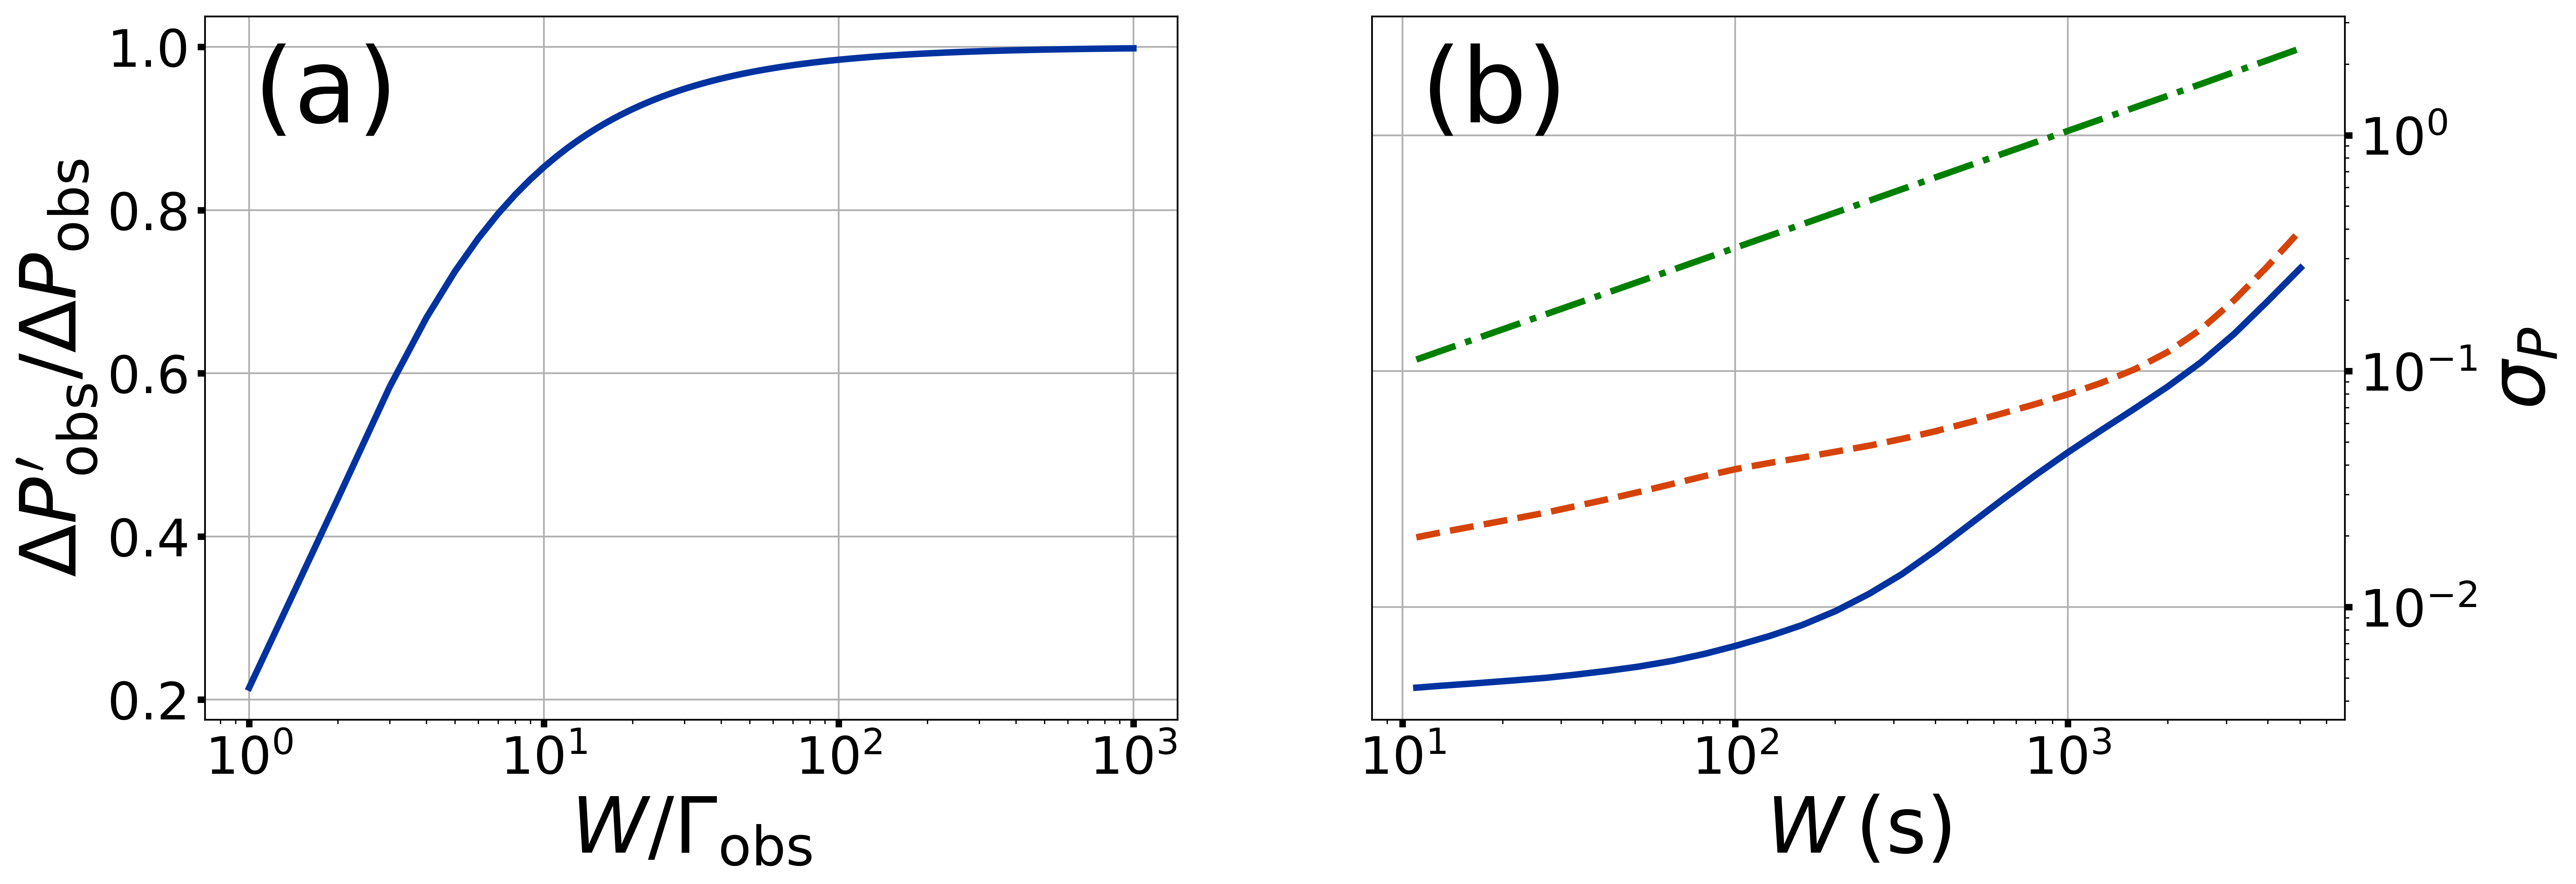
\includegraphics[width=\textwidth]{figures/Pobsprime-sigmaP_vs_W.png}
    \caption{(a) Comparing the pressure excursion observed before $\Delta P_{\rm obs}$ application of the mean boxcar filter and after $\Delta P_{\rm obs}^\prime$ as a function of the width of the filter $W$ and of the vortex signal $\Gamma_{\rm obs}$. (b) Scatter in the pressure time-series $\sigma_P$ for the sol with the largest (sol 435) and least (sol 269) values as a function of the window size $W$ for the mean boxcar filter. Sol 392 has scatter close the median value for all sols. }
    \label{fig:Pobsprime-sigmaP_vs_W}
\end{figure}

Finally, we must interpret these results in terms of our ability to recover vortices using our matched filter approach. In particular, we need to know the best shape for the matched filter: too narrow a filter might miss wider vortex profiles, while a wide filter could average out narrow profiles. To that end, we generated 500,000 synthetic time-series (200 distinct simulations for each of 2500 combinations of model parameters discussed below). These time-series had the same sampling as the APSS time-series and white noise with a wide range of variances $\sigma_\text{P}^2$. Into these time-series, we injected vortex signals with known depths and widths. Then, we applied a matched filter with width $\Gamma$ to see the range of values we retrieved for the convolution of the filter against the synthetic time-series, $\left( F \ast P \right)$. Figure \ref{fig:vortex_recovery} illustrates the range of such values and indicates that, for a very wide range of vortices, noise levels, and matched filter widths, we can successfully recover the vortices. Indeed, Figure \ref{fig:vortex_recovery} shows we could even recover very subtle vortices, given the right filter width. For example, for $\Delta P_{\rm obs}/\sigma_P$ (i.e., a vortex that barely rises above the noise), a wide range of filter widths $\Gamma$ returns $\left( F \ast P \right) \geq 5 $. The noise model discussed here does not include the non-white (red) noise that pervades the real APSS data, meaning the results are somewhat optimistic. However, based on the results here (and on additional experimentation with the real APSS time-series), we chose $\left( F \ast P \right) \geq 5 $ as our vortex detection threshold.

\begin{figure}
    \centering
    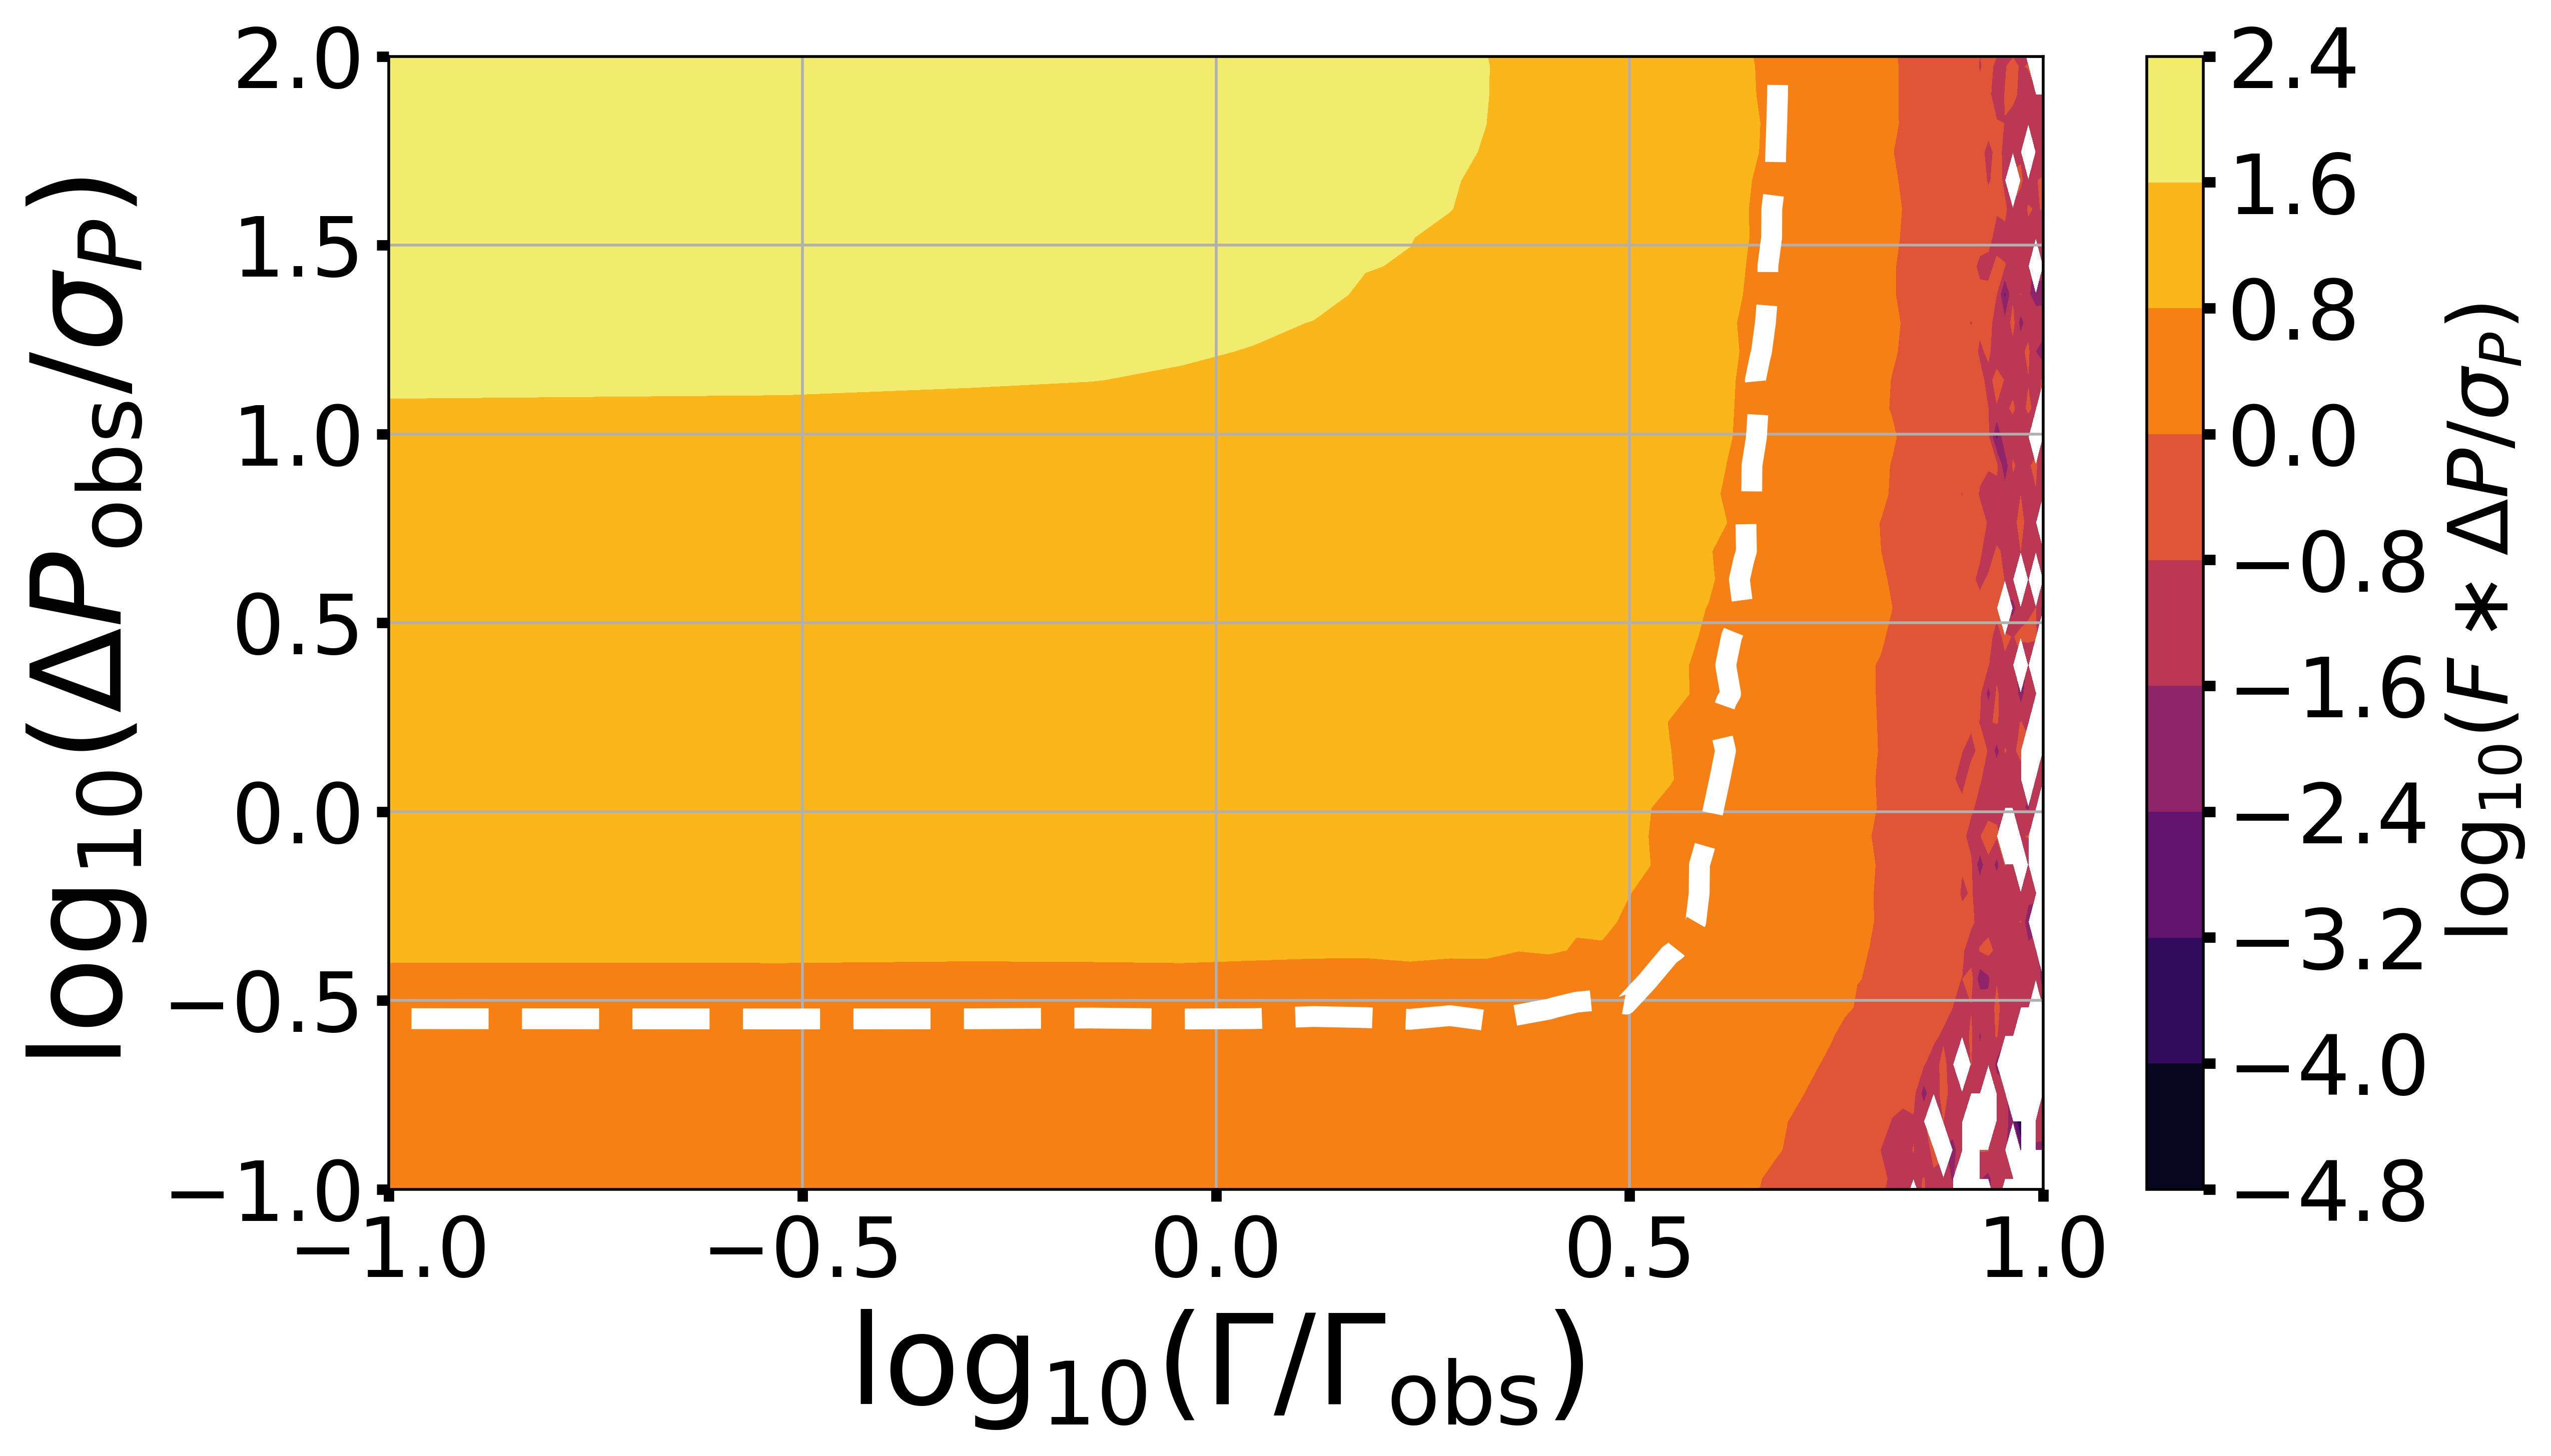
\includegraphics[width=\textwidth]{figures/vortex_recovery.png}
    \caption{How effectively a convolution of a synthetic pressure time-series with the matched filter ($F \ast P$) recovers a vortex. The vortex has a known depth $\Delta P_\text{obs}$ and width $\Gamma_\text{obs}$ and is embedded in a synthetic time-series with white noise of variance $\sigma_\text{P}^2$. The matched filtered has a width $\Gamma$. The dashed, white line shows the threshold for detection used in this study ($F \ast P \geq 5$). In principle, vortices with values of $\Delta P_\text{obs}\sigma_P$ and $\Gamma/\Gamma_\text{obs}$ above and to the left of that line could be recovered.}
    \label{fig:vortex_recovery}
\end{figure}

\section{Inferring Encounter Geometries from the Pressure and Velocity Profiles}
\label{sec:Inferring Encounter Geometries from the Pressure and Velocity Profiles}
We assume the vortices correspond to Rankine vortices \citep{1991ExFl...11...73V}, giving pressure $\Delta P$ and tangential wind velocity profiles $V$:
\begin{equation}
    \Delta P(r) = -\frac{\Delta P_{\rm act}}{1 + \left( \frac{r}{D_{\rm act}/2} \right)^2}\label{eqn:radial_lorentzian_profile}
\end{equation}
and
\begin{equation}
    V(r) = \frac{ V_{\rm act} \left( 2 \frac{r}{D_{\rm act}/2} \right)}{1 + \left( \frac{r}{D_{\rm act}/2} \right)^2},\label{eqn:radial_wind_profile}
\end{equation}
where $r$ is the radial distance from the vortex center, $P_{\rm act}$ the central pressure excursion, and $V_{\rm act}$ the peak velocity at a distance $D_{\rm act}$ from the vortex center. Equation \ref{eqn:radial_distance} shows the evolution of the radial distance with time during an encounter. At closest approach $r = b$ and we measure $\Delta P = \Delta P_{\rm obs}$ (Equation \ref{eqn:Pobs}) and 
\begin{equation}
    V = \frac{ V_{\rm act} \left( 2\frac{b}{D_{\rm act}/2} \right)}{1 + \left( \frac{b}{D_{\rm act}/2} \right)^2} = V_{\rm obs}.\label{eqn:Vobs}
\end{equation} 

Cyclostrophic balance relates the pressure and velocity as \citep{2020Icar..33813523J}:
\begin{equation}
    V_{\rm act} = \left( \Delta P_{\rm act}/\rho \right)^{1/2},\label{eqn:cyclostrophic_balance}
\end{equation}
where $\rho$ is the atmospheric density. Combining Equations \ref{eqn:Pobs}, \ref{eqn:Vobs}, and \ref{eqn:cyclostrophic_balance} gives
\begin{equation}
    \Delta P_{\rm act} = \left( 1 - \frac{\rho V_{\rm obs}^2}{4 \Delta P_{\rm obs}} \right)^{-1} \Delta P_{\rm obs},\label{eqn:solution_for_Pact}
\end{equation}
and
\begin{equation}
    V_{\rm act} = \left( 1 - \frac{\rho V_{\rm obs}^2}{4 \Delta P_{\rm obs}} \right)^{-1/2} \left( \Delta P_{\rm obs}/\rho \right)^{1/2}.\label{eqn:solution_for_Vact}
\end{equation}

We can then solve for $D_{\rm act}$:
\begin{equation}
    D_{\rm act} = \sqrt{ D_{\rm obs}^2 - \left( 2 b\right)^2 }.\label{eqn:actual_diameter}
\end{equation}

To determine the uncertainties on the actual parameters, we propagate uncertainties from the model-fit observed parameters $\sigma_{\Delta P_{\rm obs}}$, $\sigma_{D_{\rm obs}}$, $b$, and $\sigma_{V_{\rm obs}}$:
\begin{equation}
    \sigma_{\rm \Delta P_{\rm act}} = \sqrt{ \left( \frac{\partial \Delta P_{\rm act}}{\partial \Delta P_{\rm obs}} \sigma_{\Delta P_{\rm obs}} \right)^2 + \left( \frac{\partial \Delta P_{\rm act}}{\partial V_{\rm obs}} \sigma_{V_{\rm obs}} \right)^2 } = \left( \frac{\Delta P_{\rm act}}{\Delta P_{\rm obs}} \right) \sqrt{ \frac{1}{4} \rho^2 V_{\rm obs}^2 \sigma_{\Delta P_{\rm obs}}^2 + \left[ 1 + \left( \frac{\Delta P_{\rm act}}{\Delta P_{\rm obs}} \right) \left( \frac{\rho V_{\rm obs}^2}{4 \Delta P_{\rm obs}^2} \right) \right]^2 \sigma_{V_{\rm obs}}^2 }
\end{equation}
\begin{equation}
    \sigma_{\rm V_{\rm act}} = \left( \frac{\partial V_{\rm act}}{\partial \Delta P_{\rm act}} \right) \sigma_{\Delta P_{\rm act}} = \left( \frac{V_{\rm act}}{2\Delta P_{\rm act}} \right) \sigma_{\Delta P_{\rm act}}
\end{equation}
\begin{equation}
    \sigma_{D_{\rm act}} = \sqrt{ \left( \frac{\partial D_{\rm act}}{\partial D_{\rm obs}} \sigma_{D_{\rm obs}} \right)^2 + \left( \frac{\partial D_{\rm act}}{\partial b} \sigma_{b}\right)^2 } = \sqrt{ \left( \frac{D_{\rm obs}}{D_{\rm act}} \sigma_{D_{\rm obs}}\right)^2 + \left( \frac{2b}{D_{\rm act}} \sigma_{b} \right)^2 }
\end{equation}

% For N estimate, with about 6 hours per day of dust devil activity (1/4 day),
%   1 km^{-2} day^{-1} translates into about 0.25 km^{-2}.

% We can compare our estimate for the daily number of vortex encounters and the associated sampling uncertainty from Equations \ref{eqn:number_of_encounters} and \label{eqn:sigma_N} to the actual numbers reported in \citet{2020arXiv200501134S} by plugging in representative values: \citet{2020arXiv200501134S} report typical wind speeds $U \sim 5\,{\rm m\ s^{-1}}$ and vortex activity during about $12\, {\rm hours}$ each sol over about 400 sols; monitoring dust devil tracks around the InSight landing site, \citet{2020GeoRL..4787234P} suggest $N = 0.05\,{\rm km^{-2}\ sol} \times \left(12\,{\rm hours\ sol^{-1}}\right) = 0.025\,{\rm km^{-2}}$ and $D_{\rm act} \approx 10\,{\rm m}$; \citet{2018Icar..299..166J} suggests $P_{\rm act} \approx 1\,{\rm Pa}$; and our analysis here gives $P_{\rm min} \approx 0.3\,{\rm Pa}$. Taken altogether, we estimate InSight could detect vortices out to a distance $b_{\rm max} \approx 8\,{\rm m}$ distance and should have recovered about 

% 2020 May 9 - Check notes in notepad from today's date
% \section{Effects of Undersampling the Dust Devil Profile}
% With too low a sampling frequency, the pressure profile for a dust devil will be undersampled, potentially distorting the inferred profile shape and depth. Fourier analysis of the pressure profile can show the dependence of the distortion on the angular sampling frequency $\omega$.

% We start by assuming a Lorentzian profile $L(t)$ in time $t$ for the dust devil:
% \begin{equation}
%     L(t) = -\frac{\Delta P}{1 + \left( t/\Gamma \right)^2},
%     \label{eqn:appendix_lorentzian}
% \end{equation}{}
% where $\Delta P$ is the profile depth and $\Gamma$ its duration. The Fourier transform of this profile $F(\omega)$ is 
% \begin{equation}
%     F(\omega) = -\pi \Delta P\ \Gamma e^{-|\omega| \Gamma}.
%     \label{eqn:appendix_lorentzian_fourier}
% \end{equation}{}

% If we now imagine that we undersampled the profile using frequencies below some maximum, $\omega \le \omega_{\rm max}$, then we can estimate the resulting distorted profile $L^\prime(t)$ by taking the inverse, partial Fourier transform of $F(t)$, i.e.
% \begin{equation}
%     L^\prime(t) \equiv \int_{\omega = -\omega_{\rm max}}^{\omega_{\rm max}}\ \left( -\pi \Delta P \Gamma e^{-|\omega| \Gamma}\right) \ \left( \frac{e^{+i\omega t}\ d\omega}{2 \pi} \right)
%     = L(t) \bigg[ 1 - \left( \cos \left( \omega_{\rm max} t \right) - \left( \frac{t}{\Gamma} \right) \sin \left( \omega_{\rm max} t \right) \right) e^{-\omega_{\rm max} \Gamma} \bigg].
%     \label{eqn:appendix_inverse_fourier}
% \end{equation}{}

% We expect the register the maximum (in magnitude) pressure excursion at the center of the profile, i.e. $L(t = 0) = \Delta P$, and so to estimate the incorrect profile depth $\Delta P^\prime$ arising from this distorted profile, we can evaluate $L^\prime(t)$ at the same time, giving:
% \begin{equation}
%     \Delta P^\prime = \Delta P \left( 1 - e^{-\omega_{\rm max}\Gamma} \right).
% \end{equation}{}
% The distortion decreases rapidly with $\omega_{\rm max}$, and for a sampling frequency of, for example, $2\,{\rm Hz}$ ($\omega_{\rm max} = 2\pi \times (2\,{\rm Hz})$) and a very narrow profile $\Gamma = 0.5\,{\rm s}$, $\Delta P^\prime$ is only 0.2\% different from $\Delta P$.

\bibliography{sample63}{}
\bibliographystyle{aasjournal}

%% This command is needed to show the entire author+affiliation list when
%% the collaboration and author truncation commands are used.  It has to
%% go at the end of the manuscript.
%\allauthors

%% Include this line if you are using the \added, \replaced, \deleted
%% commands to see a summary list of all changes at the end of the article.
%\listofchanges

\end{document}

% End of file `sample63.tex'.